\glsreset{SB}
\chapter{Scheduling Blocks}\label{chap:scripts}

\vspace*{-0.5cm}

At the \gls{GBT}, we use \glspl{SB} to perform astronomical observations. The \gls{SB}
can contain information for configuring the telescope, balancing the \gls{IFsys}, and
other commands to \dq{tweak} the telescope system (observing directives) along with
the commands (scan types) to collect observational data. \gls{Astrid} interprets
\glspl{SB} via Python. Thus \glspl{SB} should follow Python syntax rules (such as
indentation for loops) and can also contain or make use of any Python commands.
Here is an example of a simple \gls{SB}:

\lstinputlisting[language=PythonAstrid,captionpos=b,label={lst:simplesb},caption=
{[A simple Scheduling Block]A simple \gls{SB}}]
{simple.py}

\begin{itemize}[leftmargin=*,itemsep=0pt]
\item {\bfseries{\textcolor{pythonKeywords}{execfile}}}
loads definitions for configuring the \gls{GBT}'s receivers, \gls{IFsys} and backends
for the observations.  This is described in \S~\ref{sec:config}.
\item {\bfseries{\textcolor{pythonKeywords}{Catalog}}}
loads a catalog containing information (such as positions and radial velocity, etc.) on
the sources to observe.  This is described in \S~\ref{sec:catalogs}.
\item {\bfseries{\textcolor{pythonKeywords}{Configure}}}
runs the configuration defined in {\ttfamily{myconfigurations.txt}} to select the
receiver and backend and set switches and frequencies.
This is described in \S~\ref{sec:config}.
\item {\bfseries{\textcolor{pythonKeywords}{Slew}}}
moves the telescope to the desired source (see \S~\ref{sec:scantypes}).
\item {\bfseries{\textcolor{pythonKeywords}{Balance}}}
balances the power levels in the \gls{IFsys} and backend so that they should be in their
linear regime (see \S~\ref{sec:utility}). 
\item {\bfseries{\textcolor{pythonKeywords}{Track}}}
performs and aquires data for the desired observation.  Track and other pre-defined
scans are described in \S~\ref{sec:scantypes}.
\end{itemize}

\newpage


%++++++++++++++++++++++++++++++++++++++++++++++++++++++++++++++++++++++++++++



%============================================================================
\section{Making A Scheduling Block}

{\bf \glsuserii{SB} must be created well prior to your telescope time. 
We suggest that you review \glspl{SB} with your project's contact support scientist.}

\glspl{SB} can be written using \gls{Astrid}'s \dq{Observation Management} Edit subtab
(see \S~\ref{sec:editsubtab}), which contains a simple text editor reminiscent of Notepad
(MS Windows), or you can choose to write your \gls{SB} outside of \gls{Astrid} and use the
\dq{Observation Management} Import facility in \gls{Astrid} to upload it into the database;
see \S~\ref{sec:astridimport} for details.

For the database, you should choose a descriptive name for your \gls{SB}, such as \dq{map\_G11.0}
or \dq{pointfocus}, which will remind you of the science you are trying to accomplish by running
that block. Names such as \dq{test} or \dq{turtle.p} are not descriptive and should be avoided.
The name you choose can be up to 96 characters long, and can contain white spaces, so you may
have an \gls{SB} name that consists of a few words (such as \dq{K-band frequency-switched
spectroscopy}). You do not need to add a suffix to your \gls{SB} name (*.sb or *.py).

%%%%%%%%%%%%%%%%%%%%%%%%%%%%%%%%%%%%%%%%%%%%%%%%%%%%%%%%%%%%%%%%%%%%%%%%%%%%%%

\subsection{Components of a Scheduling Block}

A typical \glsuseri{SB} will include:
\begin{enumerate}[label=\Alph*),itemsep=0pt]
\item A configuration of the system (see \S~\ref{sec:config}).
\item Specification of the sources via a catalog (see \S~\ref{sec:catalogs}).
\item A slew to the source and then balancing the power levels, and maybe other commands
(see \S~\ref{sec:utility}).
\item Observational scan type commands (see \S~\ref{sec:scantypes}).
\end{enumerate}

\noindent In the following sections we discuss each of these components.


%============================================================================
\section{Configuration of the GBT IF System}\label{sec:config}

%****************************************************************************
\subsection{Overview}

The routing of signals through the \gls{GBT} system is controlled by many electronic
switches which eliminate the need to physically change cables by hand.  The \gls{GBT}'s
electronically configurable \gls{IFsys} allows many, and more complicated paths for
the signals to co-exist at all times.  Configuring the \gls{GBT} \gls{IFsys} can
usually be accomplished in under one minute.

\subsection{Defining and Executing A Configuration}\label{sec:config_define}

\noindent Configurations are defined as sets of keyword--value pairs within a single
string variable. To execute a configuration, this variable is passed as an argument
into the {\bfseries{\textcolor{pythonKeywords}{Configure}}()} command in an \gls{SB}.
Configurations may be defined in two ways:

\begin{enumerate}
\item The configuration definition may reside on a text file external to the \gls{SB}.
It can then loaded into the \gls{SB} via the
{\bfseries{\textcolor{pythonKeywords}{execfile}()}} command
(see script~\ref{lst:config_loaded}).
\item The configuration may be explicitly defined within the \gls{SB}
(see script~\ref{lst:config_declared}).
\end{enumerate}

\newpage

We usually recommend that configuration definitions reside on text files external to
the \gls{SB}. This allows for configurations to be changed on the file without the
need to re-validate and re-save the \gls{SB} (see \S~\ref{sec:validation}). It also
allows for simple \glspl{SB} without clutter.  Note that you should always use
{\bfseries{\textcolor{pythonKeywords}{execfile}}} rather than
{\bfseries{\textcolor{pythonKeywords}{import}}}, as
{\bfseries{\textcolor{pythonKeywords}{import}}} will not reread the file and miss any
changes that you may have made.

Explicitly defining configurations within \glspl{SB} allows users to easily
edit and view their configuration from \gls{Astrid}.  If this method is chosen, users
\textbf{must} re-validate and re-save the \gls{SB} if any changes are made.  Examples
of both methods can be seen in scripts~\ref{lst:config_loaded} and
\ref{lst:config_declared}.

If using multiple configurations, it is recommended that you define them all in one
text file and load them into the \gls{SB} via a single
{\bfseries{\textcolor{pythonKeywords}{execfile}}} command. You may then use
{\bfseries{\textcolor{pythonKeywords}{Configure}}()} to execute each configuration
as necessary.

\noindent\begin{minipage}[t]{0.58\linewidth}
\lstinputlisting[captionpos=b,frame=single,framerule=1pt,language=PythonAstrid,
caption={[Basic configuration syntax]
A text file containing an example of basic configuration syntax.
},label={lst:config_syntax}]
{syntax.py}
\end{minipage}
\hfill
\begin{minipage}[t]{0.38\linewidth}
\lstinputlisting[language=PythonAstrid,captionpos=b,frame=single,
backgroundcolor=\color{sbBackground},framerule=1pt,
caption={[Loading a configuration with execfile()]
An \gls{SB} using
{\bfseries{\textcolor{pythonKeywords}{execfile}}()} to load
the contents of Script~\ref{lst:config_syntax} into \gls{Astrid}.
\dq{myconfiguration} can then be used as an argument to
{\bfseries{\textcolor{pythonKeywords}{Configure}}()} to configure the system.},
label={lst:config_loaded}]
{config_loaded.py}
\end{minipage}

\lstinputlisting[language=PythonAstrid,captionpos=b,frame=single,framerule=1pt,
backgroundcolor=\color{sbBackground},
caption={[Explicitly defining the configuration in a Scheduling Block]
An \gls{SB} that explicitly defines all configuration keywords within
triple quotes as the parameter \dq{myconfiguration}.  This parameter is then used as
an argument to {\bfseries{\textcolor{pythonKeywords}{Configure}}()} in order to configure
the system. This \gls{SB} will perform exactly the same function as the
text file and \gls{SB} shown in Scripts~\ref{lst:config_syntax} and~\ref{lst:config_loaded}.},
label={lst:config_declared}]
{config_declared.py}

\subsection{Basic Configuration Syntax}
An example of the basic configuration syntax is shown in
scripts~\ref{lst:config_syntax} and~\ref{lst:config_declared}.
Configurations are passed into {\bfseries{\textcolor{pythonKeywords}{Configure}}()} as
a string argument.  For each configuration, all keywords and values
(\S~\ref{sec:keywords}) exist as line separated keyword=value pairs,
all enclosed within a single set of triple-quotes.

\newpage

%****************************************************************************
\subsection{Example Configurations}\label{sec:examples}

The best way to learn about how to define and perform configurations is through 
examples.  Keywords available for use in a configuration definition will be 
discussed in \S~\ref{sec:keywords} and all examples have been placed in the directory,

\begin{verbatim}
/home/astro-util/projects/GBTog_examples/configs/
\end{verbatim}

%-----------------------------------------------------------------------------
\vspace*{-0.5cm}
\topic{Continuum Observations}

\lstinputlisting[language=PythonAstrid,captionpos=b,frame=single,framerule=1pt,
caption={[An example continuum configuration]
An example continuum configuration.},
label={lst:continuumconfig}]
{continuum_config.py}
\noindent
The above configuration definition (script~\ref{lst:continuumconfig}) has been given
the name \sq{continuum\_config} and can be used for pointing and focusing observations
or for continuum mapping.  We have configured for the following:


\begin{itemize}
\item \Gls{tpower}, continuum observations [obstype=\sq{Continuum}; swmode=\sq{tp};
swtype=\sq{none}].
\item The  single beam \gls{Lband} (1 to 2~GHz) receiver
[receiver=\sq{Rcvr1\_2}; beam=\sq{1}]
\item The \gls{DCR} as the backend detector [backend=\sq{DCR}]
\item {Take data using a single band centered on 1400~MHz with a 80~MHz bandwidth
      \newline [nwin=1; restfreq=1400; bandwidth=80]}
\item Go through a full switching cycle in 0.2~seconds [swper=0.2]
\item Record data with the \gls{DCR} every 0.2~seconds [tint=0.2]
\item Disable doppler tracking for continuum observations [vframe=\sq{topo};
vdef=\sq{Radio}].
\item Use a low-power \gls{noiseDiode} [noisecal=\sq{lo}]
\item Linear polarization [pol=\sq{Linear}]
\end{itemize}

%-----------------------------------------------------------------------------
\newpage

\topic{Spectral Line, Frequency Switching Observations}

\lstinputlisting[language=PythonAstrid,captionpos=b,frame=single,framerule=1pt,
caption={[An example frequency switched, spectral line configuration]
An example frequency switched, spectral line configuration.},
label={lst:fsconfig}]
{fs_config.py}

\noindent The above example (script~\ref{lst:fsconfig}) will configure for the
following:
\begin{itemize}
\item \Gls{fsw}, spectral line observations [obstype=\sq{Spectroscopy}; swmode=\sq{sp};
swtype=\sq{fsw}].
\item The single beam \gls{Lband} (1 to 2~GHz) receiver
[receiver=\sq{Rcvr1\_2}]. Note that not specifying \sq{beam} defaults to [beam=\sq{1}].
\item \gls{VEGAS} as the backend detector using linear polarization without
cross-polarization products [backend=\sq{VEGAS}; pol=\sq{Linear}].
\item Take data using a single band using \gls{VEGAS} mode 11
(see Table~\ref{tab:vegas_modes}) defined by a 23.44~MHz bandwidth, 65536 channels,
and one band per spectrometer. [bandwidth=23.44; nchan=65536; vegas.subband=1],
centered on 1420~MHz [restfreq=1420].
\item Go through a full switching cycle in 2~seconds [swper=2.0]. Over one cycle, the
\gls{fsw} states will be centered on the line, and then be shifted by -5~MHz
[swfreq=0,-5.0].
\item Record data with \gls{VEGAS} every 10~seconds [tint=10]
\item Doppler track the spectral line with the rest frequency 1420~MHz in the commonly
used Local Standard of Rest velocity with the radio definition of Doppler tracking
[vframe=\sq{lsrk}; vdef=\sq{Radio}].
\item Use a low-power \gls{noiseDiode} [noisecal=\sq{lo}]
\end{itemize}
\newpage

%-----------------------------------------------------------------------------
\topic{Multiple Spectral Lines, Total Power Observations}

\lstinputlisting[language=PythonAstrid,captionpos=b,frame=single,framerule=1pt,
caption={[An example total power, spectral line configuration]
An example total power, spectral line configuration.},
label={lst:tpconfig}]
{tp_config.py}

\noindent The above example (script~\ref{lst:tpconfig}) will configure for the
following:
\begin{itemize}
\item \Gls{tpower}, spectral line observations [obstype=\sq{Spectroscopy};
swmode=\sq{tp}; swtype=\sq{none}].
\item The single beam \gls{Xband} (8 to 10~GHz) receiver. [receiver=\sq{Rcvr8\_10}].
Note that not specifying \sq{beam} defaults to [beam=\sq{1}].
\item \gls{VEGAS} as the backend detector using circular polarization without
cross-polarization products [backend=\sq{VEGAS}; pol=\sq{Circular}].
\item Mode 21 of \gls{VEGAS} (see Table~\ref{tab:vegas_modes}).  This mode is defined
by a bandwidth of 23.44~Mhz, 8192 spectral channels in the eight subband mode of
\gls{VEGAS} [bandwidth=23.44; nchan=8192].  Note that not specifying \sq{vegas.subband}
for a bandwidth of 23.44~MHz will default to vegas.subband=8.
\item 9 spectral windows, each of which centered on one of the 9 frequencies (in MHz)
listed under restfreq [restfreq=9816.867, 9487.824, 9173.323, ....].
\item Go through a full switching cycle in 1~second [swper=1.0] and record data with
\gls{VEGAS} every 30~seconds [tint=30].
\item Doppler track the spectral line with the rest frequency 8873.1~MHz
[dopplertrackfreq=8873.1] in the commonly used Local Standard of Rest velocity
[vframe=\sq{lsrk}] with the radio definition of Doppler tracking [vdef=\sq{Radio}].
\item Use a low-power \gls{noiseDiode} [noisecal=\sq{lo}].
\end{itemize}

\newpage
%-----------------------------------------------------------------------------
\topic{Multiple Spectral Lines, Multi-beam, Total Power Observations}

\lstinputlisting[language=PythonAstrid,captionpos=b,frame=single,framerule=1pt,
caption={[An example total power, spectral line configuration for a multi-beam
receiver]An example total power, spectral line configuration for a multi-beam
receiver.},
label={lst:tpconfigmultibeam}]
{tp_config_multi_beam.py}

\noindent The above example (script~\ref{lst:tpconfigmultibeam}) will configure for
the following:
\begin{itemize}
\item \Gls{tpower}, spectral line observations [obstype=\sq{Spectroscopy};
swmode=\sq{tp}; swtype=\sq{none}].
\item The dual beam \gls{Qband} (40 to 52~GHz) receiver using both beams
[receiver=\sq{Rcvr40\_52}; beam=\sq{1,2}].
\item \gls{VEGAS} as the backend detector using circular polarization without
cross-polarization products [backend=\sq{VEGAS}; pol=\sq{Circular}].
\item Mode 2 of \gls{VEGAS} (see Table~\ref{tab:vegas_modes}).  This mode is defined
by a bandwidth of 1500~Mhz with 16384 spectral channels  [bandwidth=1500; nchan=16384].
\item 4 spectral windows, each of which centered on one of the 4 frequencies (in MHz)
listed under restfreq [restfreq=44580, 43751, 45410, 46250].
\item Shift the window centered on 43751~MHz by 100~MHz in the local (topocentric)
frame.  Thus, this window will now be centered on 43851~MHz [deltafreq=0,100,0,0].
deltafreq should be defined in the same manner as restfreq: This example uses 4 comma
separated values.
\item Go through a full switching cycle in 1~second [swper=1.0] and record data with
\gls{VEGAS} every 10~seconds [tint=10].
\item Doppler track the spectral line with the rest frequency 44580~MHz (default is
the first specified rest frequency) in the commonly used Local Standard of Rest
velocity [vframe=\sq{lsrk}] with the radio definition of Doppler tracking [vdef=\sq{Radio}].
\item Use a low-power \gls{noiseDiode} [noisecal=\sq{lo}].
\end{itemize}
\newpage

%-----------------------------------------------------------------------------
\topic{Multiple Spectral Lines, KFPA Observations}
\vspace{-0.1cm}
\lstinputlisting[language=PythonAstrid,captionpos=b,frame=single,framerule=1pt,
caption={[An example total power, spectral line configuration for the KFPA]
An example total power, spectral line configuration for the \gls{KFPA}.},
label={lst:kfpaconfig}]
{kfpa_config.py}

\vspace{-0.1cm}
\noindent The above example (script~\ref{lst:kfpaconfig}) will configure for the
following:
\vspace{-0.1cm}
\begin{itemize}
\item \Gls{tpower}, spectral line observations [obstype=\sq{Spectroscopy};
swmode=\sq{tp}; swtype=\sq{none}].
\item The \gls{KFPA} (18 to 26~GHz) receiver using all 7 beams
[receiver=\sq{RcvrArray18\_26}; beam=\sq{all}].
\item \gls{VEGAS} as the backend detector with circular cross-polarization products
[backend=\sq{VEGAS}; vegas.vpol=\sq{cross}; pol=\sq{Circular}].
\item {Mode 4 of \gls{VEGAS} (see Table~\ref{tab:vegas_modes}).  This mode is defined by
a bandwidth of 187.5~Mhz with 32768 spectral channels [bandwidth=187.5; nchan=32768].}
\item {3 spectral windows centered on 24600, 23900, and 25500~MHz.  Data will be recorded
for beams 1$\rightarrow$4 using the first window (24600~MHz) while beams 5$\rightarrow$7
will use the second window (23900~MHz).  An additional \gls{IFpath} will be routed
from beam 1 to the window centered on 25500~MHz.  This is known as the \dq{7+1} mode of the
\gls{KFPA} (see Chapter~\ref{chap:kfpa}) [restfreq={24600:\sq{1,2,3,4},23900:\sq{5,6,7},
25500:\sq{-1},\sq{DopplerTrackFreq}: 24700}].}
\begin{itemize}
\item {Note that doppler tracking the center (24700~MHz) of the full frequency range
(25500-23900+bandwidth) is necessary in this example.  The maximum frequency separation
limitation of the \gls{KFPA} is 1.8~GHz when using multiple beams
(see Chapter~\ref{chap:kfpa}).  The Radio definition of doppler tracking has been used
in the Local Standard of Rest Velocity [vframe=\sq{lsrk}; vdef=Radio]}
\end{itemize}
\item Shift the window centered on 24600~MHz by -100~MHz in the local (topocentric)
frame.  Thus, this window will now be centered on 24500~MHz
[deltafreq={24600:-100, 23900:0, 25500:0}].  deltafreq should be defined using the same
syntax as restfreq: This example uses Python dictionary syntax.
\item Go through a full switching cycle in 1~second [swper=1.0] and record data with
\gls{VEGAS} every 30~seconds [tint=30].
\item Use a low-power \gls{noiseDiode} [noisecal=\sq{lo}].
\end{itemize}
\newpage

\topic{Advanced Use of the Restfreq Keyword}

\lstinputlisting[language=PythonAstrid,captionpos=b,frame=single,framerule=1pt,
caption={[An example showing advanced use of the restfreq keyword]
An example showing advanced use of the restfreq keyword.},
label={lst:advrestfreqconfig}]
{adv_restfreq_config.py}

The above example (Script~\ref{lst:advrestfreqconfig}) uses the advanced restfreq
syntax (an array of Python dictionary terms) to more precisely configure the
\gls{GBT} system.  Note that this is an example of usage only and it is not recommended
that users attempt to manually route beams to specific \gls{VEGAS} banks.

When using the advanced restfreq syntax, it is important to be aware of the following
details in the main configuration block:
\begin{itemize}[itemsep=0pt]
\item Key values specified in the restfreq dictionary term override key-values
pairs in the main configuration.  If no values for a key have been specified, a
default value will be used if available.
\item {\bf bandwidth} and {\bf nchan} must always be specified in the main
configuration block outside of restfreq.  This is required for the configuration to
pass validation, even if such values are redundant [bandwidth=23.44; nchan=32768].
\item {\bf dopplertrackfreq} must be set by the user [dopplertrackfreq=13500.0]
since there is no default doppler tracking frequency for the advanced restfreq syntax.
\end{itemize}

\newpage

\noindent
The following points give details on the usage of the advanced restfreq syntax in
this example:
\begin{itemize}
\item Multiple rest frequencies (or windows centered on a rest frequency) are input
as an array of Python dictionary terms.  The \sq{{\bf restfreq}} dictionary key
is the minimum required entry for each dictionary term and specifies the center of
each window.  Each bank may also be configured with different resolution, bandwidth,
and number of spectral windows.  However, the integration time, switching period and
frequency switch must be the same for all banks.
\item Each window may be routed to a specific bank (\gls{VEGAS} spectrometer) with
the \sq{{\bf bank}} dictionary key (see the first window of this example).
By omitting \sq{bank}, the system will attempt to route windows to available
banks automatically (recommended).
Note that certain restrictions exist when routing multi-beam receivers to \gls{VEGAS}
banks.  See \S~\ref{sec:vegas_if} and \S~\ref{sec:kfpa_configuration} for further
information.

\item The \sq{{\bf beam}} dictionary key specifies which beam is used for the
      window. Omitting \sq{beam} defaults to beam 1 [\sq{beam}:\sq{1}].
\item {\gls{VEGAS} modes are set for a window by defining valid combinations of
      bandwidth and resolution, and the number of sub-bands if using a 23.44~MHz
      bandwidth (see Table~\ref{tab:vegas_modes}). If these values are not defined
      as dictionary keys, then values defined in the main configuration block or
      default values will be used. It is worth noting the following points in this
      example:}
  \begin{itemize}
  \item {Bank C has been split into 3 subbands and uses \gls{VEGAS} mode 23
        defined by 23.44~MHz bandwidth, 8 subbands, and 0.7~kHz resolution
        [\sq{bank}:\sq{C}, \sq{bandwidth}:23.44, \sq{res}:0.7, \sq{subband}:8].
        The 3 windows are centered on 13200, 13300, and 13400~MHz.
        {\bf Note that all sub-bands within a single bank must use identical
        \gls{VEGAS} settings apart from the center frequency and offset}.}
  \item A second window has been centered around 13400~MHz using a bandwidth of
        23.44~MHz with 0.7~kHz resolution. However, this window is configured to
        use beam 2 and mode 10 of \gls{VEGAS} with a single sub-bank
[{\sq{restfreq}:13400,\sq{bandwidth}:23.44,\sq{res}:0.7,\sq{beam}:\sq{2},\sq{subband}:1}]
  \item The window centered at 13100~MHz gives an example of the
        other dictionary keys available.  This window has been shifted +1~MHz
        in the local frame [\sq{deltafreq}:1] to be centered on 13101~MHz.  Data
        will be recorded with full Stokes polarization products [\sq{vpol}:\sq{cross}].
        All other windows will record data with total intensity polarization
        products [vegas.vpol=\sq{self} (the default setting)]
  \end{itemize}

\end{itemize}

\newpage

%****************************************************************************
\subsection{Configuration Keywords}\label{sec:keywords}

%-----------------------------------------------------------------------------
\subsubsection{Keywords That Must Always Be Present}

The following keywords do not have default values and must be present
in all configuration definitions.

\begin{description}[leftmargin=*,font=\bfseries\large]

\item[receiver] This keyword specifies the  name of the \gls{GBT}\ receiver to be used.
The names and frequency ranges of the receivers can be found in Table~\ref{table:rx}.
The value of the receiver keyword is a string and should therefore be placed within
quotes when used.

\begin{table}[!h]
\begin{center}
\setlength{\abovecaptionskip}{0pt}\setlength{\belowcaptionskip}{0pt}
\caption[GBT receivers and frequencies]
{\gls{GBT} receivers and their nominal frequency ranges.
\label{table:rx}}
\begin{tabular}{lll}
\toprule
Name    & Frequency Range (GHz) & Notes             \\
\midrule
Rcvr\_342       &   .290--.395  & \gls{PFone} feed\\
Rcvr\_450       &   .385--.520  & \gls{PFone} feed\\
Rcvr\_600       &   .510--.690  & \gls{PFone} feed\\
\midrule
Rcvr\_800       &   .680--.920  & \gls{PFone} feed\\
Rcvr\_1070      &   .910--1.23  & \gls{PFtwo}         \\
Rcvr1\_2        &   1.15--1.73  & \gls{Lband}       \\
\midrule
Rcvr2\_3        &   1.73--2.60  & \gls{Sband}       \\
Rcvr4\_6        &   3.95--7.8   & \gls{Cband}       \\
Rcvr8\_10       &   8.00--10.0  & \gls{Xband}       \\
\midrule
Rcvr12\_18      &   12.0--15.4  & \gls{Kuband}      \\
RcvrArray18\_26 & 18.0--26.5    & \gls{KFPA} 7-beam focal plane array \\
Rcvr26\_40      &  26--31, 30.5--37, 36--40 & \gls{Kaband} \\
\midrule
Rcvr40\_52      &   40.5--47.0  & \gls{Qband} \\
Rcvr68\_92      & 67--74, 73--80, 79--86, 85--93 & \gls{Wband} \\
Rcvr\_PAR       & 80---100 & \gls{MUSTANG} Bolometer Array\\
NoiseSource     &  N/A & \\
\bottomrule
\end{tabular}
\end{center}
\end{table}

\item[backend] This keyword specifies the name of the backend (data acquisition
system) to be used.  The value for this keyword is a string.  Valid backends are
listed in Table~\ref{table:backends}.

\begin{table}[!h]
\setlength{\abovecaptionskip}{0pt}\setlength{\belowcaptionskip}{0pt}
\begin{center}
\caption[GBT backends]{\gls{GBT}\ backends.\label{table:backends}}
\begin{tabular}{@{}l p{\dimexpr 0.65\linewidth-2\tabcolsep}}
\toprule
Name & Notes \\ \midrule
DCR & The Digital Continuum Receiver directly from the \gls{IFRack}.\newline
One frequency available.\\
\midrule
DCR\_AF & The Digital Continuum Receiver from the \gls{AFRack} \newline
          Four/two frequencies maximum for single/dual beam receivers. \\
\midrule
VEGAS  & Spectral line backend with up to 524288 channels and 64 \newline
frequencies with various bandwidths.\\
\midrule
VLBA\_DAR & Very Long Baseline Array Data Acquisition Recorder.\\
\midrule
Radar & For bi-static radar observations. Private backend.\\
\midrule
CCB & CalTech Continuum Backend  \\
\midrule
GUPPI  & Green Bank "Ultimate" Pulsar Processor.  \\
\bottomrule
\end{tabular}
\end{center}
\end{table}

\newpage

\item[obstype] This keyword specifies the type of observing to be performed.  The
allowed values are one of the following strings: \sq{Continuum},
\sq{Spectroscopy}, \sq{Pulsar}, \sq{Radar}, \sq{VLBI}.

\item[bandwidth] This keyword gives the bandwidth in MHz to be used by the
specified backend.  The value of the keyword should be a float.  Possible values
depend on the receiver and backend that are chosen (see Table~\ref{table:bw} and
Table~\ref{tab:vegas_modes}).

\begin{table}[!h]
\begin{center}
\caption[Allowed bandwidths]
{Allowable bandwidths for backends.\label{table:bw}}
\begin{tabular}{ll p{\dimexpr 0.3\linewidth-2\tabcolsep}}
\toprule
Backend  &  Receiver & Possible Bandwidths (MHz)\\
\midrule
VEGAS & Any & 1500, 1000, 187.5, 100, \newline
                    23.44, 16.9, 11.72 \\
\midrule
DCR, VLBI, or Radar  & Prime Focus  & 20, 40, 80, 240  \\
\midrule
DCR, VLBI, or Radar  & 
Rcvr1\_2, Rcvr4\_6, Rcvr8\_10, Rcvr12\_18  & 20, 80, 320, 1280  \\
\midrule
DCR, VLBI, or Radar  &
Rcvr2\_3, RcvrArray18\_26, Rcvr40\_52  & 80, 320, 1280  \\
\midrule
DCR\_AF  & Any  & 12.5, 50, 200, 800  \\
\midrule
CCB & Rcvr26\_40 & 600 \\
\midrule
GUPPI    & Any & 100, 200, 800 \\
\bottomrule
\end{tabular}
\end{center}
\end{table}


\item[restfreq]

This keyword specified the rest frequencies for spectral line observations or
the center frequencies for continuum observations.  There are three available
syntaxes for restfreq:

\begin{enumerate}[label=\bfseries{\arabic*.},leftmargin=*]
\item {\bf Simple}

\begin{lstlisting}[language=PythonAstrid,frame=single,framerule=1pt]
restfreq  = 1420, 1661, 1667
deltafreq = 0, 5, 0
\end{lstlisting}
The above example sets 3 rest frequencies and offsets the
second window (1661~MHz) by +5~MHz in the local (topocentric) frame using deltafreq.
Rest frequencies may be specified as a list of comma separated float values (MHz).
This syntax should be used when all beams (including single beam receivers) are
configured to observe the same rest frequencies and \gls{VEGAS} does not need to
use an advanced configuration (see \dq{Advanced} below).  Note that:

\begin{itemize}[itemsep=0pt]
\item {\bf deltafreq} can also specified using the same syntax as restfreq, a
single global offset, or ommitted to use the default value of zero.
\item If {\bf dopplertrackfreq} is not set in the main configuration block then the
first rest frequency listed using this syntax will be doppler tracked by
default.
\end{itemize}

\item {\bf Multi-beam}
\begin{lstlisting}[language=PythonAstrid,frame=single,framerule=1pt]
restfreq={24000:'1,2,3,4',23400:'5,6',25000:'7',
          'dopplertrackfreq':24200}
#deltafreq must be specified with this syntax - even when zero
deltafreq = {24000:0, 23400:0, 25000:0}
\end{lstlisting}
The above example specifies a rest frequency of 24000~MHz for beams 1--4, 23400~MHz
for beams 5 and 6, and 25000~MHz for beam 7.
Different feeds of multi-beam receivers may be tuned to different rest frequencies.
Rest frequencies and delta frequencies are input as Python dictionaries.  Further
information on this syntax and example can be found in
Appendix~\ref{appendix:spectralwindows}.  Note that:

\begin{itemize}[itemsep=0pt]
\item {\bf deltafreq} must {\bf always} be specified as a separate Python dictionary, even when
zero.
\item {\bf dopplertrackfreq} must {\bf always} be specified in the restfreq Python dictionary.
\end{itemize}

\newpage
\item {\bf Advanced}

\begin{lstlisting}[language=PythonAstrid,frame=single,framerule=1pt]
bandwidth = 23.44
nchan     = 32768
dopplertrackfreq = 1420.0
restfreq = [{'restfreq':1420.0},
            {'restfreq':1420.0,'deltafreq':-20.0},
            {'restfreq':1667.0,'bandwidth':11.72,'nchan':65536}]
\end{lstlisting}

The above example will configure \gls{VEGAS} to use 3 rest frequencies.  The first
two windows are centered on 1420~MHz with mode 23 of \gls{VEGAS} using
bandwidth=23.44 and nchan=32768 from the main configuration block
(8 subbands are selected by default for bandwidth=23.44). However, deltafreq has been
used as a dictionary key to offset the second window by -20~MHz in the local topocentric
frame.  A third window is centered on 1667~MHz with mode 16 of \gls{VEGAS} using
the \sq{bandwidth} and \sq{nchan} dictionary keys to override values from the main
configuration block.

This syntax may be used to more precisely configure \gls{VEGAS} observations and
specifies restfreq as an array of Python dictionaries.  See script~\ref{lst:advrestfreqconfig}
for a more detailed example of this syntax.  Note that:

\begin{itemize}
\item Available dictionary keys are: \sq{\bf{restfreq}}, \sq{\bf{bandwidth}},
\sq{\bf{nchan}}, \sq{\bf{res}}, \sq{\bf{deltafreq}}, \sq{\bf{tint}}, \sq{\bf{vpol}},
\sq{\bf{bank}}, \sq{\bf{beam}}, and \sq{\bf{subband}}.
\begin{itemize}[itemsep=0pt]
\item \sq{\bf{restfreq}} takes a float value in MHz and is the only required key for
each dictionary term.
\item \sq{\bf{res}} is the spectral resolution (kHz) and can be used as an alternative
to the \sq{nchan} restfreq dictionary key or the \sq{nchan} keyword in the main
configuration block to select the \gls{VEGAS} mode. Allowed values are floats and
listed in Table~\ref{tab:vegas_modes}.
\item \sq{\bf{bank}} specifies which \gls{VEGAS} bank to use.  Allowed values are the
string letters \sq{A}$\rightarrow$\sq{H}.  The default is to let the configuration tool
select which bank should be used (recommended).
\item All other keys have the same meaning as the standard configuration keywords.
\end{itemize}

\item Key-value pairs specified in the dictionary override configration keywords specified
in the main configuration block which in turn override any default values.
\item {\bf dopplertrackfreq} must {\bf always} be set in the main configuration block.
\item {\bf deltafreq} may still be specified as a single global offset in the main
configuration block or ommitted to use the default value of zero.
\item {\bf nchan} must {\bf always} be set in the main configuration block, even if that
value is overridden by \sq{nchan} in the restfreq dictionary.
\end{itemize}

\end{enumerate}

%herez
\end{description}
\newpage

%-----------------------------------------------------------------------------
\subsubsection{Keywords With Default Values}
\begin{description}[font=\bfseries\large,leftmargin=*,align=right]

\item[swmode] This keyword specifies the switching mode to be used for the
observations.  This keyword's values are given as a string.
The switching schemes are
\begin{itemize}
\item {\bf \sq{tp}: } (Total Power With Cal) - The \gls{noiseDiode} is
periodically turned on and off for equal amounts of time. {\bf (Default value)}
\item {\bf \sq{tp\_nocal}: } (Total Power Without Cal) - The \gls{noiseDiode}
is turned off for the entire scan.
\item {\bf \sq{sp}: } (Switched Power With Cal) - The \gls{noiseDiode} is
periodically turned on and off for equal amounts of time while another
component is in a signal state and then again in a reference state.  This is
used in \gls{fsw} where the signal state is one frequency and the reference
state is another frequency.  Similarly \gls{bsw} and \gls{polsw} change the
beams or polarizations so that their signals are sent down two different
\glspl{IFpath}.
\item {\bf \sq{sp\_nocal}: } (Switched Power Without Cal) - The
\gls{noiseDiode} is turned off while another component is switched between
a signal and reference state.
\end{itemize}

\item[swtype] This keyword is only used when swmode=\sq{sp} or
swmode=\sq{sp\_nocal},  and specifies the type of switching to be performed. 
This keyword's values are \sq{none}, \sq{fsw} (\gls{fsw}), \sq{bsw} 
(\gls{bsw}) and \sq{psw} (\gls{polsw}). {\bf Default values
are \sq{fsw} for all receivers except receiver='Rcvr26\_40'.
The default for receiver='Rcvr26\_40' is swtype='bsw'.} 

\item[swper] This keyword defines the period in seconds  over which the full
switching cycle occurs. See Table~\ref{tab:blanking_cal} for recommended
minimum switching periods for each \gls{VEGAS} mode.  The value is a float.
{\bf Default values are 0.2 for obstype='continuum', 0.04 for
obstype='pulsar', and 1.0 for any other value for the obstype keyword}. 

\item[swfreq]  This keyword defines the frequency offsets used in \gls{fsw}
(swtype=\sq{fsw}).  The value consists of two comma separated floats which
are the pair of frequencies in MHz. The best values for swfreq are
bandwidth/$2^{n}$ where $n$ is an integer so that the frequency switch will
be an integer number of channels giving less artifacts in data reduction.
{\bf Default values are swfreq=-0.25*Bandwidth, +0.25*Bandwidth for 
swtype='fsw', and swfreq=0,0 otherwise.}

\item[tint] This keyword specifies the backend's integration (dump) time.
The value is a float with units of seconds. See Table~\ref{tab:vegas_modes}
for minimum integration times with \gls{VEGAS}.
{\bf Default values are 10.0 for obstype='continuum', tint=swper for
obstype='spectroscopy' and 30.0 of any other value for the obstype
keyword.}

\item[beam]  {This keyword specifies which beams are to be used for
observations with multi-beam receivers.   The keyword value is a string
of comma separated integers.  For example beam='2' would record data for
the second beam and beam='3,7' would record data for beams 3 and 7.
When using the \gls{KFPA}, beam='all' can be used to record
data from all seven beams. This \sq{beam} configuration keyword has a
different meaning to the \sq{beamName} in observing scans which usually
specifies a tracking beam, not which beams to record data for.
{\bf The default value is \sq{1}}.}
\begin{itemize}
\item [{\bf Note:}] The \gls{Kaband} dual-beam single-polarization 26--40~GHz
receiver (\sq{Rcvr26\_40}) has a unique architecture among \gls{GBT} receivers.
The two beams are routed through the \gls{IFsys} as if they are two
polarizations of a single beam.  Therefore, the only allowable setting for
\sq{beam} with \sq{Rcvr26\_40} is beam='1'.
\end{itemize}

\item[nwin] {This keyword specifies the number of frequency windows that will
be observed for backends other than \gls{VEGAS}. The value for this keyword
is an integer with a maximum value that is backend and receiver dependent,
see \S~\ref{sec:backends}. The number of values given for
the restfreq keyword must be the same as nwin.  {\bf The default value is 1}.}
\begin{itemize}
\item [{\bf Note:}] \sq{nwin} does not need to be specified for \gls{VEGAS}
configurations.
\end{itemize}

\item[deltafreq] This keyword specifies offsets in MHz for each spectral
window so that the restfreq is not centered in the middle of the spectral
window. \sq{deltafreq} can be specified as a single float offset which
will be applied across all windows or in the same manner as \sq{restfreq}.
For examples of using deltafreq with different types of restfreq syntax, see
Scripts~\ref{lst:tpconfigmultibeam},~\ref{lst:kfpaconfig},
and~\ref{lst:advrestfreqconfig}.  More details on deltafreq can be found in
Appendix~\ref{appendix:spectralwindows}.  {\bf The default value is 0.0}.


\item[vframe]  This keyword specifies the velocity frame (the inertial
reference frame).  The keyword value is a string.  Allowed values
are \sq{topo} (topocentric, i.e. Earth's surface), \sq{bary}
(Barycenter of solar system), \sq{lsrk} (Local Standard of Rest kinematical
definition , i.e. typical LSR definition), \sq{lsrd} (Local Standard of Rest 
dynamical definition -- rarely used), \sq{galac} (center of galaxy), \sq{cmb} 
(relative to Cosmic Microwave Background).
{\bf The default value is \sq{topo}.}

\item[{\bf \large vdef}] This keyword specifies which mathematical equation
(i.e. definition) is used to convert between frequency and velocity.  The
keyword value is a string.  Allowed values are \sq{Optical}, \sq{Radio},
\sq{Relativistic}. {\bf The default value is \sq{Radio}.}
\begin{equation}
\gls{vradio} = c \left[ 1 - {\nu \over \nu_o} \right]
\label{eq:vradio}
\end{equation}
\begin{equation}
\gls{voptical} = c \left[ {\nu_o \over \nu} - 1\right]
\label{eq:voptical}
\end{equation}
\begin{equation}
\gls{vrelativistic} = c \left[ {\nu_o^2 - \nu^2 \over \nu_o^2 + \nu^2} \right]
\label{eq:vrel}
\end{equation}
%$${\rm  \gls{vred} = {z \over c} }$$  
 

\end{description}


%-----------------------------------------------------------------------------
\subsubsection{Backend and Receiver Dependent Keywords}

Some configuration keywords depend on which backends and receivers are being
used.  Some observations may require one of these keywords while for other
observations none may be needed.

\begin{description}[font=\bfseries\large,leftmargin=*]

\item[nchan] An integer.  This keyword is used to determine the number of
spectral channels that \gls{VEGAS} will provide.  Available values are listed
in Table~\ref{tab:vegas_modes}.

\begin{itemize}
\item[-] The following string values designed for use with the now obsolete
\gls{GBT} spectrometer may still be used: \sq{low}, \sq{medium-low}, \sq{medium},
\sq{medium-high}, and \sq{high}.  These string values may be used to distinguish
between up to 5-levels of resolution for a given bandwidth.  For example, mode
18 of \gls{VEGAS} could be set by setting bandwith=11.72 and nchan=262144 or
nchan='medium-high'.
\end{itemize}

\item[dopplertrackfreq] A float specifying the rest frequency in MHz used to
compute the velocity for doppler tracking.  When using the simple restfreq
syntax, the default is the first listed restfreq value.

\item[pol]  Each of the prime focus receivers, \gls{Lband}, \gls{Sband}
and \gls{Cband} receivers have a hybrid that can output either linear
or circular polarization. This keyword specifies whether linear or
circular polarization is desired for these receivers. The keyword value
is a string.  Allowed values are \sq{Linear} and \sq{Circular}.
{\bf The default value is \sq{Circular} for the \glsunset{VLBI}\gls{VLBI}
and Radar back ends, and \sq{Linear} otherwise.}

\item[noisecal]  All receivers below 12~GHz have two noise
diodes for calibration signals -- one with an equivalent brightness
temperature at roughly one tenth the system temperature (\sq{lo} value) and
one nearly equal to the system temperature (\sq{hi} value).  This keyword is
a string which specifies which noise diode is to be used.  Allowed
values\footnote{There are expert values of \sq{on-mcb}, \sq{on-ext}, \sq{lo-mcb}, 
\sq{hi-mcb}, \sq{lo-ext} and \sq{hi-ext} whose use is beyond the scope of this
document.  Please contact a support person about the use of these values.}
are \sq{lo}, \sq{hi} and \sq{off}. {\bf The default value is \sq{lo} except
for the Radar backend for which the default values is \sq{off}.}

For the \gls{Kaband} (26-40~GHz) receiver there are three additional choices.
These are \sq{L}, \sq{R}, or \sq{LR}.  The \gls{Kaband} receiver has two
\sq{lo} noise diodes, one for each polarization for each of the two beams.  The
\sq{L}, \sq{R}, and \sq{LR} options specify which of these noise diodes are to
be used.

\item[notchfilter]  There is a notch filter covering roughly 1200--1310~MHz
in the \gls{Lband} receiver that filters out an \glsunset{FAA}\gls{FAA} radar
signal.  This keyword determines if this notch filter is in place and used
by the system or is removed from the receiver's \gls{RF} path.  The keyword
value is a string with allowed values of \sq{In} or \sq{Out}.
{\bf The default value is \sq{In}.}

\item[vegas.vpol] Keyword to specify which spectral product to record in the
FITS file. It assumes the following values:

\begin{itemize}
\item {\bf \sq{self}:} Record the total intensity polarization products.
{\bf (Default value)}
\item {\bf \sq{cross}:} Record the full Stokes polarization products.
\item {\bf \sq{self1}:} Record the polarization from the first \glsfirst{ADC}
card only. There are two \glspl{ADC} per \gls{VEGAS} bank, one for each
polarization.
\item {\bf \sq{self2}:} Record the polarization from the second \gls{ADC} only.
\end{itemize}

\item[vegas.subband] Keyword used by config tool to select between
23.44~MHz \gls{VEGAS} modes with single and multiple spectral windows (see
Table~\ref{tab:vegas_modes}). It assumes values 1 or 8.
{\bf The default value is 8.}

\item[guppi.obsmode] {\gls{GUPPI}-specific keyword (see Chapter~\ref{chap:GUPPI}).
Controls both the dedispersion and observing mode. All data are written in
format.  Allowed values are}
    \begin{itemize}
    \item \textbf{\sq{search}:} Incoherent search-mode, i.e. spectra are
        rapidly written to disk.
    \item \textbf{\sq{fold}:} Incoherent fold-mode, i.e. spectra are are
        folded on-line using a pulsar ephemeris, with sub-integrations
        written to disk at a rate controlled by the
        \textbf{guppi.fold\_dumptime} keyword.  \emph{Note: incoherent
          fold-mode is effectively deprecated in favor of coherent
          fold-mode.}
    \item \textbf{\sq{cal}:} Incoherent cal-mode, i.e. data are folded at a
        constant 25 Hz frequency; used in conjunction with the pulsed
        noise diodes for each receiver.
    \item \textbf{\sq{coherent\_search}:} Coherent search-mode,
        i.e. spectra are coherently dedispersed at a DM specified
        using the \textbf{guppi.dm} keyword before being channelized,
        accumulated, and written to disk.
    \item \textbf{\sq{coherent\_fold}:} Coherent fold-mode, i.e. spectra
        are coherently dedispersed at the DM specified in the
        ephemeris file before being written to disk.  Since the DM is
        read from the ephemeris file, the guppi.dm keyword is not
        needed.
    \item \textbf{\sq{coherent\_cal}:} Coherent cal-mode, i.e. data are
        taken as in coherent fold mode, although no dedispersion is
        applied since the noise diode is not dispersed.
    \end{itemize}

\item[guppi.polnmode] controls whether Full Stoke's or total
    intensity data are recorded.  Allowed values are
    \sq{\textbf{full\_stokes}} and \sq{\textbf{total\_intensity}},
    though total intensity can only be used in incoherent search-mode.
\item[guppi.numchan] sets the number of spectral channels.
    Allowed values are \textbf{any power-of-two between 64 and 4096},
    though care must be taken not to exceed the maximum data rate.
\item[guppi.outbits] controls the number of bits used for
    output values.  The only allowed value is \textbf{8}.
\item[guppi.scale] controls the internal scaling so that the
    output data is properly scaled for 8-bit values.  This value is
    typically chosen from experience with the observing set-up.
    Contact your project friend for advice on which value to use.
\item[guppi.datadisk] controls which RAID data are written to
    in incoherent modes.  Allowed values are \sq{\textbf{data1}} or
    \sq{\textbf{data2}}. In coherent modes data are written to eight
    HPC machines and this keyword is not used. It will go in a subdirectory
    called {\bf /guppi.datadisk/observername/projectID/date/}.
    Since the data will be owned by the \dq{monctrl} computer account,
    you will not be able to remove it -- that means Scott Ransom will bug
    you mercilessly until you process your data!
\item[guppi.fold\_parfile] specifies the path to the ephemeris
    (parfile) used for either incoherent or coherent fold-modes.
    \emph{The parfile must exist and be visible from beef, and readable by tempo.}
\item[guppi.dm] controls the DM used for coherent search-mode.  It is not
     used by any other modes.
\item[guppi.fold\_bins] controls the number of phase bins used
    for either incoherent or coherent fold- or cal-modes.  Enough bins
    should be used to fully resolve fine profile structure.  Typical
    values are 256 in incoherent modes (which are not typically used
    anymore) and 2048 in coherent modes.
\item[guppi.fold\_dumptime] controls the length of a
    sub-integration in either incoherent or coherent fold- or
    cal-modes.  The value is specified in seconds, with 10 s being
    typical.  It must be shorter than the total scan length.
\item[vlbi.phasecal] This expert keyword turns the \gls{VLBI} phase
cals on or off.  The phase cals can can run at 1~MHz (\sq{M1}) or
5~MHz (\sq{M5}). The keyword value is a string.  Allowed values are
\sq{off}, \sq{M1} or \sq{M5}.
\item[broadband] This keyword is used to activate the \dq{broadband}
7.5~GHz maximum instantaneous mode of the \gls{KFPA} by setting
{\tt broadband=1}.  This may only be used with single beam configurations
using either beam 1 or beam 2.  The default is \dq{off} (\tt broadband=0).

\end{description}

%-----------------------------------------------------------------------------
\subsubsection{Expert Keywords}

These keywords should only be used by very experienced observers who
have expert knowledge of how a given backend works or in how the \gls{GBT}
\gls{IFsys} works.

\begin{description}[font=\bfseries\large,leftmargin=*]

\item[vlow \textnormal{and} vhigh] These keywords specify the minimum
and maximum velocity to be observed from a group of sources.  The value is a
float and is in ${\rm km~s^{-1}}$ for velocities. See
Appendix~\ref{appendix:vlowhigh} for more details on the use of vlow and
vhigh.  The use of vlow and vhigh is not recommended for frequencies where
there can be large amounts of \gls{RFI}. {\bf The default value is 0.0.}

\item[iftarget] This keyword specifies the target voltage level to use
when balancing the \gls{IFRack}.  The keyword value is a float.  The nominal
range of the \gls{IFRack} is 0.0--10.0 and the linear range is 0.1--5.0.


\item[xfer] This expert keyword sets the beam switch for the 
\gls{Kuband}, \gls{Kband} and \gls{Kaband} receivers.  The keyword is a string.
Allowed values are \sq{ext}, \sq{thru}, or \sq{cross}.  The default values are
\sq{ext} when swtype=\sq{bsw} and \sq{thru} otherwise.

\item[polswitch]  This expert keyword sets the polarization switch
for the \gls{Lband} and \gls{Xband} receivers.  The keyword value is a string.
Allowed values are \sq{ext}, \sq{thru}, and \sq{cross}.  The default value is
\sq{ext} if swtype=\sq{psw} and \sq{thru} otherwise.

\item[ifbw] This expert keyword sets the minimum \gls{IF} bandwidth to be
used in filters within the receiver and in the \gls{IFRack}.  The keyword value
is float with units of MHz.

\item[if0freq] This expert keyword is used to set the center frequency
of the \gls{IF} after the mixing the \gls{RF} signal with the first
\gls{LO}.  The keyword value is a float with units of MHz.

\item[lo1bfreq] This expert keyword is used to set the frequency of
the synthesizer used for the alternative \gls{LOone}, LO1B.  This keyword is
only to be used with the \gls{Kaband} receiver.  The keyword value is a float
with units of MHz.

\item[lo2freq] This expert keyword is used to set the frequency
values of the eight \gls{LOtwo} synthesizers within the \gls{CRRack}.  
The keyword values are a comma separated list of floats with units 
of MHz.

\item[if3freq] This expert keyword is used to set the \gls{IF} input
frequency of the backend.  The keyword value is a comma separated list of
floats with units of MHz.

\end{description}

\subsection{Resetting The Configuration}\label{sec:reset}

The configuration tool in \gls{Astrid} remembers all the keyword values
defined during a session. This feature occasionally results in \gls{Astrid}
being unable to validate an otherwise correct configuration because of
previously set values or hardware being configured improperly.
To reset the configuration parameters to their default state, you can
issue the  {\bfseries{\textcolor{pythonKeywords}{ResetConfig}}()} command
in a script before another
{\bfseries{\textcolor{pythonKeywords}{Configure}}()}. This command will
reset the configuration tool values to their defaults.

\newpage

%============================================================================

\section{Catalogs}\label{sec:catalogs}

The Source Catalog system in \gls{Astrid} provides a convenient way for the user 
to specify a list of sources to be observed, as well as a way to refer to 
standard catalogs of objects.  At a minimum for each source there must be a 
name and a location (Ra/Dec or Glat/Glon, etc). Other parameters may be 
set, such as radial velocity.
An example of a simple Catalog is:

\lstinputlisting[language=PythonAstrid,captionpos=b,
frame=single,framerule=1pt,backgroundcolor=\color{catalogBackground},
caption={[A simple catalog]A simple catalog.},
label={lst:simple_catalog}]
{simple_catalog.cat}

\noindent There are three formats of catalogs:
\begin{itemize}
\item {\bf SPHERICAL} A fixed position in one of our standard coordinate
systems, e.g., RA/DEC, AZ/EL, GLON/GLAT, etc.
\item {\bf EPHEMERIS} A table of positions for moving sources (comets,
asteroids, satellites, etc.)
\item {\bf NNTLE NASA/NORAD} \gls{TLE} sets for earth satellites.
\end{itemize}

In addition, the following solar system bodies may be referred to by name:
\dq{Sun}, \dq{Moon}, \dq{Mercury}, \dq{Venus}, \dq{Mars}, \dq{Jupiter},
\dq{Saturn}, \dq{Uranus}, \dq{Neptune}, and \dq{Pluto}. These names are
case-insensitive and may be given to any Scan Type function
(see \S~\ref{sec:scantypes}). No catalog needs to be  invoked for the system
to understand these names.

To use the catalog system, observers invoke the
{\bfseries{\textcolor{pythonKeywords}{Catalog}}()} command within \glspl{SB}
and pass names of the desired objects to any of the scan functions
(\S~\ref{sec:scantypes}). All sources named in all the catalogs that have
been invoked are available within an \gls{SB}. If the same name appears in
two or more catalogs, the name from the most recently invoked catalog will
prevail. Name comparisons are case-insensitive, hence \dq{b2322+16} and
\dq{B2322+16} are equivalent.

%****************************************************************************
\subsection{Getting Your Catalog Into Astrid}

Although one can include any number of Catalogs in an \gls{SB}, the standard
practice is to put all the Catalogs into separate files that are then brought
into the \gls{SB} via multiple calls to the
{\bfseries{\textcolor{pythonKeywords}{Catalog}}()} command. This: a) keeps
\glspl{SB} simple and without clutter; and b) allows changes to be made
to a Catalog without having to validate and re-save the \gls{SB}.

The best way to learn about how to bring Catalogs into an \gls{SB} is through
an example. Let's suppose that there are two Catalogs that you need for your
observations.  These two catalogs are in the following files:

\begin{verbatim}
/home/astro-util/projects/GBTog_examples/cats/sources.cat
/home/astro-util/projects/GBTog_examples/cats/pointing.cat
\end{verbatim}

\newpage
These catalogs may be loaded into the \gls{SB} as shown in the following
example:

\lstinputlisting[language=PythonAstrid,captionpos=b,
frame=single,framerule=1pt,backgroundcolor=\color{sbBackground},
caption={[Loading catalogs into Scheduling Blocks]
Loading two catalogs into an \gls{SB}, then using objects
defined in those catalogs as inputs to scan functions},
label={lst:catalog_loaded}]
{catalog_loaded.py}

All sources from all catalogs are available and referenced by name within
the scope of the \gls{SB}, with the exception that for duplicate  source
names only the last entry of that name will be recognized. After loading
a Catalog any scan function may be run by giving it the source name as
shown above (Script~\ref{lst:catalog_loaded}).

%****************************************************************************
\subsection{The Format of the Catalog}

A Catalog typically has two sections: a header section followed by a table
of information for all the sources. The header section consists of
\dq{KEYWORD = VALUE} pairs.  The \dq{KEYWORD = VALUE} pairs tell the
\glsuseri{SB} interpreter how to read the information in the table section
of the Catalog.  Once a keyword value is given, its value will persist
until re-set or the end of the Catalog is reached.  The keywords are
case-insensitive.  The values for a keyword  must not contain any embedded
blanks (except source names in NNTLE format).

A Catalog can contain comments with the beginning of a comment being denoted
by the hash symbol, \dq{\#}. All information on a line after the hash symbol
is considered to be part of the comment. After the header, each source in
the Catalog occupies a single line. You should not use the hash symbol in source
names.

%-----------------------------------------------------------------------------
\topic{Catalog Header Keywords}

Catalog Header Keywords are used to define how the catalog entries should
be read.  The keywords and their values are case insensitive. The example
shown in Script~\ref{lst:header_keywords} will be used to describe some of
the Catalog Header Keywords.  Unless mentioned otherwise, the following keywords
should be listed as column headings under \dq{HEAD}:

\lstinputlisting[language=PythonAstrid,captionpos=b,keepspaces=true,
frame=single,framerule=1pt,backgroundcolor=\color{catalogBackground},
caption={[Catalog header keywords]An example catalog using additional header keywords},
label={lst:header_keywords}]
{header_keywords.cat}

\newpage
\begin{description}[leftmargin=*,font=\bfseries\large]
\item[FORMAT] This tells the type of catalog and {\bf must be the first
line in any catalog}. Possible values are \dq{spherical}, \dq{ephemeris} 
and \dq{nntle}.  For the SPHERICAL format, the first line would 
contain \dq{FORMAT=SPHERICAL}. This is the default format, hence the 
\dq{FORMAT=SPHERICAL} may be omitted.

\item[HEAD] This gives the header for tabular data,
and consists of a list of any keywords. This should appear as the last
line in the header before lines giving information about the sources in
the catalog.  You can also create your own header keyword, such as the
\dq{type} column in the above example.  The default header is
\dq{HEAD = NAME RA DEC VELOCITY}. In the above example we have added
more entries than the default.  We have also created a new keyword named
\dq{type}.

\item[NAME] The source name is any string up to 32 characters long.
The name should not contain any embedded blanks or hashes.

\item[COORDMODE] The default is J2000. Possible values are:
J2000, B1950, JMEAN (mean coordinate of date given by EQUINOX), GAPPT 
(geocentric apparent coordinates of date), GALACTIC, HADEC, AZEL, ENCODER.
In the above example we put the COORDMODE keyword in the HEAD line since
we have sources whose positions are given in different coordinate modes
(J2000 and B1950).  This keyword may be given as either a header keyword
or columnn heading under \dq{HEAD}.

\item[VEL \textnormal{or} VELOCITY] The radial velocity in km/sec. 
The Default is to use any previous setting or 0.0 if there is none.

\item[VELDEF] Velocity definition in the FITS convention, e.g. 
\dq{VOPT-BAR}, \dq{VRAD-LSR}, etc.
(see \htmladdnormallink
{https://safe.nrao.edu/wiki/bin/view/GB/Data/VelDefFits}
{https://safe.nrao.edu/wiki/bin/view/GB/Data/VelDefFits}).
The default is the velocity definition or reference frame that was previously set.
In the above example we put the VELDEF keyword in the HEAD line since we have
sources whose velocity definitions are different. This keyword may be given as
either a header keyword or columnn heading under \dq{HEAD}. This value will
also override the velocity definition in the configuration (see \S~\ref{sec:keywords}).

\item[RESTFREQ] The rest frequency, in MHz. The default is to use the previous
setting.  Again we put the RESTFREQ keyword in the HEAD line since we are
defining two different spectral line rest frequencies for each source.  Note
that this is an \dq{expert} keyword as one has to be aware of any conflicts
with the hardware configuration. This keyword may be given as either a header
keyword or columnn heading under \dq{HEAD}.

\item[RA, HA, DEC, AZ, EL, GLON, GLAT] A pair of coordinates must be given:
RA/DEC, HA/DEC, AZ/EL, or GLON/GLAT. Angle formats may be either in sexegesimal
with colons (e.g. dd:mm:ss.ss) or in decimal format.  RA and HA are always in
hours regardless of decimal or sexegesimal notation, while all other coordinates
use degrees or arc in both formats.

\item[EQUINOX] Used if the Coordmode is \dq{JMEAN}.  The value
is a float (e.g. 2006 December 1, 12:00 UT would be 2006.919178082192).
This keyword may be given as either a header keyword or columnn heading
under \dq{HEAD}.
\end{description}

\lstinputlisting[language=PythonAstrid,captionpos=b,keepspaces=true,
frame=single,framerule=1pt,backgroundcolor=\color{catalogBackground},
caption={[Catalog equinox header keyword]
An example catalog using the equinox header keyword.},
label={lst:equinox}]
{equinox.cat}

\newpage
\begin{itemize}[leftmargin=*]
\item Additional keywords used when the Ephemeris format is active are
(see \S~\ref{sec:ephemeris} for examples):
\end{itemize}

\begin{description}[leftmargin=*,font=\bfseries\large]

\item[DATE] The UTC date, either \dq{2005-06-23} or \dq{2005-Jun-23} form.
This keyword may be given as either a header keyword or columnn heading
under \dq{HEAD}.

\item[UTC] The UTC time in the form \dq{hh:mm:ss}.

\item[DRA, DHA, DDEC, DAZ, DEL, DLON, DLAT]
The coordinate rate keywords given in arc-seconds per hour.

\item[DVEL] The radial velocity rate in km/sec/hour.

\end{description}

\begin{itemize}[leftmargin=*]
\item Additional keywords used by the NNTLE format are (see \S~\ref{sec:nntle} 
on NNTLE format below for examples):
\end{itemize}

\begin{description}[leftmargin=*,font=\bfseries\large]

\item[FILE]  For use in NNTLE format only. This keyword value may refer to
a file or a URL containing a 2-line element set.  This keyword may not be
listed as a column name under \dq{HEAD}.

\item[USERADVEL] For use in the NNTLE format only. If this is set to 1, 
then the radial velocity tracking will be performed.  Otherwise, if this is 
set to 0 or is missing then radial velocity tracking will not be performed.
This keyword may not be listed as a column name under \dq{HEAD}.

\end{description}



%****************************************************************************
\subsubsection{SPHERICAL format Examples}

--Here is an example of a simple catalog.

\lstinputlisting[language=PythonAstrid,captionpos=b,
frame=single,framerule=1pt,backgroundcolor=\color{catalogBackground},
caption={[A simple spherical format catalog]A simple catalog.},
label={lst:spherical_catalog}]
{simple_catalog.cat}

\noindent --Because all the keyword values use the defaults, the
following is equivalent:

\lstinputlisting[language=PythonAstrid,captionpos=b,
frame=single,framerule=1pt,backgroundcolor=\color{catalogBackground},
caption={[Catalog default header keywords and columns]
A simple catalog using default header keywords and columns.},
label={lst:default_header_catalog}]
{default_header_catalog.cat}

\newpage

\noindent --Here is an example catalog that specifies the radial
velocities of the sources.

\lstinputlisting[language=PythonAstrid,captionpos=b,keepspaces=true,
frame=single,framerule=1pt,backgroundcolor=\color{catalogBackground},
caption={[Catalog velocity column]
A catalog using the \dq{velocity} column to specify radial velocity
in km/sec.},
label={lst:radial_velocities_catalog}]
{radial_velocities.cat}

\vspace*{0.25cm}
\noindent --Here is an example Catalog where  one may omit the \dq{format=} 
line, but not the \dq{coordmode=} line.

\lstinputlisting[language=PythonAstrid,captionpos=b,keepspaces=true,
frame=single,framerule=1pt,backgroundcolor=\color{catalogBackground},
caption={[Catalog using Galactic coordinates]
A catalog using the \dq{Galactic} coordinate mode and omitting
\dq{format=}.},
label={lst:galactic_catalog}]
{galactic.cat}
\vspace*{-0.25cm}
{\bf Warning:} setting the velocity or rest frequency in a catalog only
changes the values in the \gls{LOone} manager. If either value is changed
by a large amount, the receiver selection or bandpass filters or the
frequency spacing between spectral windows may change. Thus one should
re-configure the \gls{IFsys} for a large change in velocity or frequency. The 
user should be wary of how much the velocity or rest frequency can change for 
a particular configuration.

\vspace*{0.5cm}
\noindent --Finally we show an example Catalog with user-defined keywords.
The user may create custom keywords (or equivalently column headings). 
These are available within an \gls{SB}, but are otherwise ignored.

\lstinputlisting[language=PythonAstrid,captionpos=b,keepspaces=true,
frame=single,framerule=1pt,backgroundcolor=\color{catalogBackground},
caption={[Catalog user--defined keywords]A catalog with user--defined keywords},
label={lst:custom_catalog}]
{custom_keywords.cat}

\newpage

%****************************************************************************
\subsection{Standard Catalogs}

Several \dq{standard} catalogs listed in Table~\ref{table:catalogs} are
available for use within the Green Bank computing system. They are all ASCII
files in the directory {\verb!/home/astro-util/astridcats!}.

Note that for convenience, these standard catalogs may be referred to within
Astrid simply by name, without the \dq{.cat} extension. e.g.:

\lstinputlisting[language=PythonAstrid,captionpos=b,keepspaces=true,
frame=single,framerule=1pt,backgroundcolor=\color{sbBackground},
caption={[Loading standards catalogs into Astrid]
Loading standard catalogs into an \gls{SB}},
label={lst:standard_catalog}]
{standard_catalog.cat}

\vspace{0.2cm}

\begin{table}[!h]
\begin{center}
\caption[Available catalogs]{The following Catalogs are present as of April 
2016. The flux densities of pointing calibrators vary by up to a factor of 
two on time scales of years at frequencies higher than 8 GHz, so the pointing 
calibrators will never be good flux calibrators. The main reason for 
updating their flux  densities is to make sure the observer gets a 
strong-enough pointing calibrator. For genuine flux-density calibration, we
recommend observers use the flux densities of 3C123, 3C286, and 3C295
(See Perly and Butler, 2013).\label{table:catalogs}\\}
\begin{tabular}{l p{\dimexpr 0.7\linewidth-2\tabcolsep}}
\toprule
Catalog & Description \\ \midrule

fluxcal &
Calibrators with well-determined flux densities. U.~S.~Government Printing
Office (Usgpo) 2006, The Astronomical Almanac for the year 2006, Washington:
U.S.~Government Printing Office (USGPO), 2006, U.S.~Naval Observatory (USNO),
Royal Greenwich Observatory (RGO). \\ \midrule

pointing &
Condon's master pointing catalog for the \gls{GBT}. \newline
\htmladdnormallink{https://safe.nrao.edu/wiki/bin/view/GB/PTCS/PointingFocusCatalog}
{https://safe.nrao.edu/wiki/bin/view/GB/PTCS/PointingFocusCatalog} \\ \midrule
pf\_pointing & Extracted from pointing catalog for the 50 cm band (0.6GHz). \\
lband\_pointing & Extracted from pointing catalog for the 21 cm band (1.4GHz). \\
sband\_pointing & Extracted from pointing catalog for the 10 cm band (3GHz). \\ 
cband\_pointing & Extracted from pointing catalog for the 6 cm band (6GHz). \\
xband\_pointing & Extracted from pointing catalog for the 3.5 cm band (9GHz). \\
kuband\_pointing & Extracted from pointing catalog for the 2 cm band (14GHz). \\
kband\_pointing & Extracted from pointing catalog for the 1.5 cm band (20GHz). \\
kaband\_pointing & Extracted from pointing catalog for the 9 mm band (32GHz). \\
qband\_pointing & Extracted from pointing catalog for the 7 mm band (43GHz). \\ 
wband\_pointing & Extracted from pointing catalog for the 3.5mm band (86GHz). \\
mustang\_pointing & Extracted from pointing catalog for the 3.3mm band (90GHz). \\
\midrule
HI\_strong &
Galaxies with strong HI lines, extract from Rich Fisher's database.\newline
\htmladdnormallink{http://www.gb.nrao.edu/\~{}rfisher/GalaxySurvey/galaxy\_survey.html}
{http://www.gb.nrao.edu/~rfisher/GalaxySurvey/galaxy_survey.html} \\ \midrule
pulsars\_all &  All 1533 pulsars in the ATNF database as of 26 Aug 2005. \\
pulsars\_all\_GBT &  All 1054 pulsars visible from Green Bank. \\
pulsars\_brightest\_GBT &  The brightest pulsars, visible from Green Bank. \\
pulsars\_bright\_MSPs\_GBT &  Bright millisecond pulsars visible from Green Bank. \\
\bottomrule
\end{tabular}
\end{center}
\end{table}

\newpage

The GBT pointing catalog has been updated several times to  include
better positions and more recent flux densities.  These changes are
described in the PTCS project notes posted at \newline
\htmladdnormallink{https://safe.nrao.edu/wiki/bin/view/GB/PTCS/ProjectNotes}
{https://safe.nrao.edu/wiki/bin/view/GB/PTCS/ProjectNotes}

\begin{itemize}[leftmargin=*]
\item PTCS/PN/58 introduces PCALS4.1 and \dq{gold standard} pointing 
calibrators for use at higher frequencies

\item PTCS/PN/66 introduces PCALS4.4, a catalog upgrade incorporating 
high-frequency flux densities from WMAP5 and accurate positions from the 
VLBA calibrator surveys through VCS6

\item PTCS/PN/72 introduces PCALS4.5 with high-frequency flux densities 
updated by WMAP7, the Planck `\dq{Early Release Compact Source Catalog}, and 
the Australia Telescope AT20G survey.

\item PCALS 4.7 adds new 30, 44, 70, and 100 GHz flux densities from the 
final Planck Catalogue of Compact Sources (Planck Collaboration, 2013 
( arXiv:1303.5088) and 20 GHz fluxes from Righini, S., Carretti, E., 
Ricci, R. et al. 2012 MNRAS, 426, 2107 \dq{A 20 GHz bright sample for 
delta $> +72^\circ$: I. Catalogue}.  
There is no PTCS/PN describing this release.

\end{itemize}




%****************************************************************************
\subsection{Catalog Functions}
Two useful catalog functions are available.

\topic{c.keys()}

Acts like a Python function that returns a list of all the source names
in the Catalog loaded into the variable \sq{c} [i.e. via
c={\bfseries{\textcolor{pythonKeywords}{Catalog}}}(\sq{mycatalog})].
The value returned can be used in the \gls{SB} to automatically loop
through all the sources in a catalog.  Here is an example of how to do this:

\lstinputlisting[language=PythonAstrid,captionpos=b,keepspaces=true,
frame=single,framerule=1pt,backgroundcolor=\color{sbBackground},
caption={[Catalog c.keys() function]
Using c.keys() to create an array of source names in the \gls{SB}},
label={lst:catalog_func1}]
{catalog_func1.py}

\topic{c[\sq{sourcename}][\sq{keyword}]}

Returns the value of the keyword for the named source in the Catalog loaded
into the variable \sq{c}. This function can be used to pass information in
the Catalog on to the \gls{SB} (e.g. specifying different map sizes for
different sources/directions).

The c[\sq{sourcename}][\sq{keyword}] function can be used to get information
out of the \dq{keyword} column of the Catalog for use within the \gls{SB}.
In the following example we get the source's Declinations and only observe
those sources above $20^\circ$ Declination (note that the coordinates are
always returned in degrees):

\lstinputlisting[language=PythonAstrid,captionpos=b,keepspaces=true,
frame=single,framerule=1pt,backgroundcolor=\color{sbBackground},
caption={[Using a catalog function to retrieve the declination of a source]
An example \gls{SB} that retrieves the declination of each source
in the catalog and prints it to screen.  If the declination of the source is
above 20$^\circ$ then the \gls{SB} will proceed to perform a\
{\bfseries{\textcolor{pythonKeywords}{Nod}}()} scan.},
label={lst:catalog_func2}]
{catalog_func2.py}

The c[\dq{sourcename}][\dq{keyword}] function can also be used to execute
more complicated observing strategies.  In the following example we have
many sources to observe and we desire a different amount of total
integration time for each source.  To accomplish this we add two new
columns to the Catalog.  We will call these columns \dq{sourcetime}
and \dq{status}.  A few lines of the Catalog (lets call it mycatalog.cat)
would look like:

\lstinputlisting[language=PythonAstrid,captionpos=b,keepspaces=true,
frame=single,framerule=1pt,backgroundcolor=\color{catalogBackground},
caption={[Catalog user--defined columns]
An example catalog with user--defined columns.},
label={lst:mycatalog}]
{mycatalog.cat}

\noindent The \gls{SB} would look like:
\lstinputlisting[language=PythonAstrid,captionpos=b,keepspaces=true,
frame=single,framerule=1pt,backgroundcolor=\color{sbBackground},
caption={[Retrieving information from Catalog user--defined columns]
An example \gls{SB} that retrieves information for each
source from user-defined columns in the catalog shown in
Script~\ref{lst:mycatalog}.},
label={lst:catalog_func3}]
{catalog_func3.py}

{\bf Note that c[\sq{sourcename}][\sq{keyword}] will return a string value}.
Thus, we convert \dq{dwelltime} in Script~\ref{lst:catalog_func3} to a
float value in order to use it as a suitable time argument in the
{\bfseries{\textcolor{pythonKeywords}{Track}}} scan function.

%****************************************************************************

\subsection{EPHEMERIS : Tables for moving objects}\label{sec:ephemeris}

A Catalog can also be used as an Ephemeris for the position of a moving object,
such as a comet or asteroid.  To make the Catalog into an Ephemeris the first
non-comment line of the Catalog must contain:
\begin{verbatim}
FORMAT = EPHEMERIS
\end{verbatim}
The header of the Catalog for an Ephemeris can also contain the NAME,
COORDMODE, VELDEF and HEAD keywords.
The \dq{data lines} in the Catalog must contain at least the date, the time, 
and a pair of coordinates for an Ephemeris.   Optional parameters are 
coordinate rates, radial velocity and radial velocity rate.  User-defined 
parameters may also be added.

The dates and times are required to be in UTC. The dates and times can 
be specified in any legal python form, for example:
a) 'YYYY-MM-DD hh:mm:ss' where MM is month number (e.g ${\rm August = 09}$);
or b) 'YYYY-MMM-DD hh:mm:ss' where MMM is the abbreviated month name such as 
Jan, Feb, etc.

The ephemeris table should contain enough entries to cover a period longer 
than that required by a particular observing session with sufficient time
resolution for the expected motion with respect to the telescope's beam
size.  The observing system selects the portion of the table needed for
the current scan start time and duration.

\newpage
\subsubsection{Example Ephemeris Catalogs}

\lstinputlisting[language=PythonAstrid,captionpos=b,keepspaces=true,
frame=single,framerule=1pt,backgroundcolor=\color{catalogBackground},
caption={[A simple ephemeris catalog]A simple ephemeris catalog.
Note that the \dq{HEAD=} line has been omitted because the default
is \dq{DATE UTC RA DEC VEL}},
label={lst:ephemeris1}]
{ephemeris1.cat}

\lstinputlisting[language=PythonAstrid,captionpos=b,keepspaces=true,
frame=single,framerule=1pt,backgroundcolor=\color{catalogBackground},
caption={[A ephemeris catalog with coordinate rates]
A more complicated ephemeris catalog for a comet that specifies the
coordinate rates.},
label={lst:ephemeris2}]
{ephemeris2.cat}

\lstinputlisting[language=PythonAstrid,captionpos=b,keepspaces=true,
frame=single,framerule=1pt,backgroundcolor=\color{catalogBackground},
caption={[A ephemeris catalog for tracking a satellite]
A ephemeris catalog for tracking a satellite.},
label={lst:ephemeris3}]
{ephemeris3.cat}

\newpage

%****************************************************************************
%Instructions for getting ephemeris from JPL.
\subsubsection{Comets}\label{sec:comets}

Tracking a comet which does not track at the sidereal rate will require the 
use of an external file generated from the NASA JPL Horizons website which 
holds a database of all the orbital parameters of all major and minor bodies 
in the solar system. First you must download the ephemeris file for your 
object of interest from the website: 
\htmladdnormallink{http://ssd.jpl.nasa.gov/horizons.cgi}
{http://ssd.jpl.nasa.gov/horizons.cgi}.
Then you will have to convert the file into the CATALOG format for astrid.

When you go to \htmladdnormallink{http://ssd.jpl.nasa.gov/horizons.cgi}
{http://ssd.jpl.nasa.gov/horizons.cgi} you should see something
like what is shown in Figure \ref{fig:jplweb}.

\begin{figure}[!h]
\begin{center}
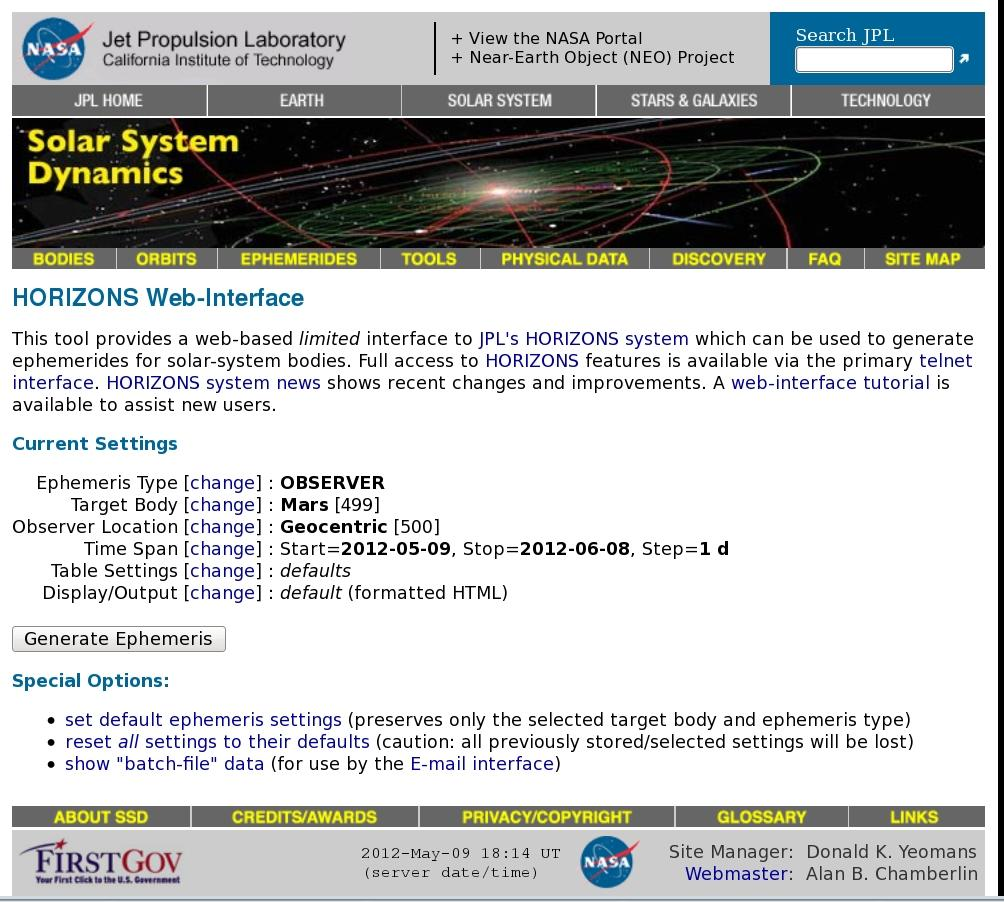
\includegraphics[width=\linewidth]{jplHorizon.jpg} 
\caption{The JPL Horizons website \label{fig:jplweb}}
\end{center}
\end{figure}

\newpage
\noindent Your entries in the \dq{Current Settings} should be:
\begin{description}[leftmargin=*]
\item [Ephemeris Type:] OBSERVER
\item [Target Body:] SELECT YOUR OBJECT \\
      Clicking on the blue [change] link will open a form to search for
      the object of interest.
\item [Observer Location:] Green Bank (GBT) [-9] (radar) 
      ( 280� 09' 36.7''E, 38� 25' 59.1''N, 873.10~ m) \\
      To set the location to Green Bank, first click [change], then
      select \dq{Observatories}, click \dq{Display List}, and select
      \dq{Green Bank (GBT) [-9] (radar)}. \\
\item [Time Span:] CHOOSE YOUR RANGE \\
The ephemeris table should contain enough entries to cover a period longer 
than that required by a particular observing session. The observing system 
selects the portion of the table needed for the current scan start time and 
duration.  If the position of the comet is changing rapidly, you should 
select a \dq{step} range of 5 mins or shorter.  If the comet is further out 
in the solar system and is not moving as rapidly with respect to the sidereal 
rate, a \dq{step} range of 10-15 mins may be adequate to track the comet.  
Consult your observatory friend if you are unsure of the step range you 
should choose. \\
\item [ Table Setting:] QUANTITIES=1,3,20 \\
Figure \ref{fig:jplTableSettings} shows the quantities that should be 
selected through the web interface to properly generate an ephemeris for
tracking a comet. NOTE: The dates and times are required to be in UTC.
The dates and times can be specified in any legal python form, for
example: a) 'YYYY-MM-DD hh:mm:ss' where MM is month number (e.g August = 09);
or b) 'YYYY-MMM-DD hh:mm:ss' where MMM is the abbreviated month name such
as Jan, Feb, etc. (see below)
\end{description}

\begin{figure}[!h]
\begin{center}
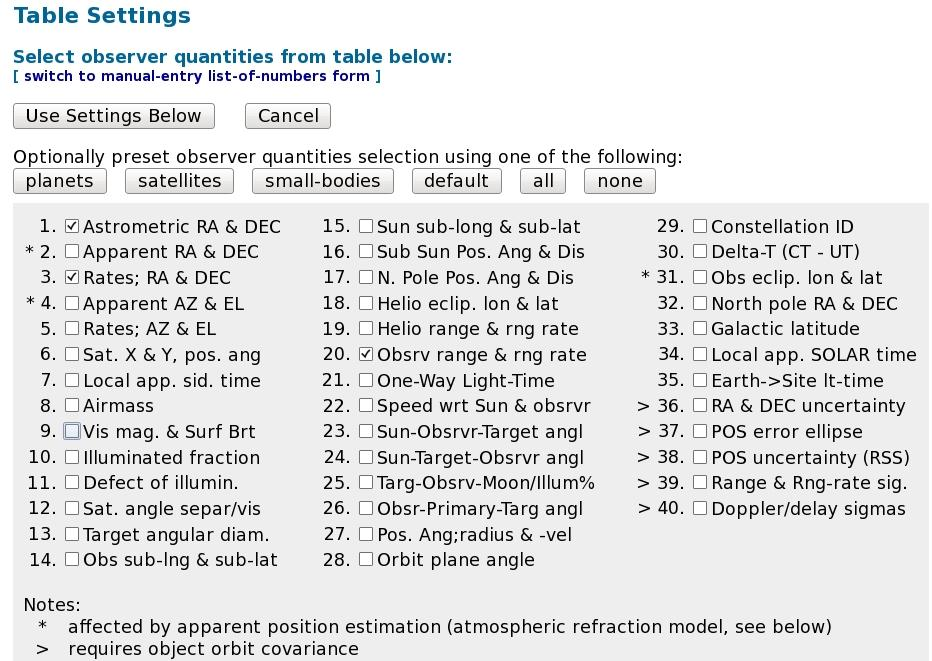
\includegraphics [height=3.0in] {jplTableSet2.jpg}
\caption {Selecting quantities to generate an ephemeris.
\label{fig:jplTableSettings}}
\end{center}
\end{figure}

\begin{description}[leftmargin=*]
\item [ Display/Output:] download/save
\end{description}

\newpage
After clicking \dq{Generate Ephemeris}, you should save the file to a directory
in your area in Green Bank.  The ephemeris file will begin with a large amount of
header information followed by lines containing the date, time and pairs of
coordinates as shown in Script~\ref{lst:JPLephem}. Optional parameters are
coordinate rates, geocentric distance and geocentric radial velocity.

\lstinputlisting[captionpos=b,keepspaces=true,basicstyle=\ttfamily\scriptsize,
frame=single,framerule=1pt,backgroundcolor=\color{white},
caption={[JPL ephemeris file]A JPL ephemeris file},
label={lst:JPLephem}]
{JPLephem.txt}

\newpage

Now that you have your ephemeris, it needs to be converted to a form that
\gls{Astrid} can read. You can do this by running the Python script 
{\verb!jpl2astrid!} from any directory in your area on the Green Bank computer
system. If you just type \dq{jpl2astrid}, and give it no arguments, it lists 
instructions, like this:

\lstinputlisting[captionpos=b,keepspaces=true,basicstyle=\ttfamily\footnotesize,
frame=single,framerule=1pt,backgroundcolor=\color{white},
caption={[jpl2astrid usage]jpl2astrid usage},
label={lst:jpl2astrid_usage}]
{jpl2astrid_usage.txt}


If you give it a file name, say by typing \dq{jpl2astrid jplephemfile.txt},
it produces another file in the form for \gls{Astrid} Catalogs. You should
verify that the first non-comment line of the resulting catalog file 
contains:

\begin{verbatim}
FORMAT = EPHEMERIS 
\end{verbatim}

You now have a valid catalog file that \gls{Astrid} will be able to use.
When you load the catalog into \gls{Astrid}, make sure you have the
correct path and that the name of the comet is exactly what is in
the .astrid catalog file in \dq{quotations}.
The catalog file should look something like this:

\lstinputlisting[language=PythonAstrid,captionpos=b,keepspaces=true,
frame=single,framerule=1pt,backgroundcolor=\color{catalogBackground},
lastline=10,
caption={Astrid catalog generated by jpl2astrid]
An \gls{Astrid} ephemeris catalog for generated by running
jpl2astrid on Script~\ref{lst:JPLephem}},
label={lst:JPLastridCatalog}]
{horizons_results.astrid}

{\bf Note:} You may wish to edit the \dq{NAME =} line to rename the
object.  The name of the object will be used in \glspl{SB} as an
argument to scan functions such as
{\bfseries{\textcolor{pythonKeywords}{Track}}}.

\newpage

%****************************************************************************

\subsection{NNTLE : Tracking Earth satellites}\label{sec:nntle}

\dq{NNTLE} stands for NASA/NORAD Two-Line Elements. This refers to a standard 
NASA format for orbital elements for Earth satellites (see 
e.g.~\htmladdnormallink{http://ghrc.msfc.nasa.gov/orbit/tleformat.html}
{http://ghrc.msfc.nasa.gov/orbit/tleformat.html} or \\
\htmladdnormallink{http://www.amsat.org/amsat/keps/formats.html}
{http://www.amsat.org/amsat/keps/formats.html}).  The first non-comment
line of the Catalog must contain:
\begin{verbatim}
FORMAT = NNTLE
\end{verbatim}

If the FILE keyword is used then one should only give the name of the object
in the Catalog as the elements of the orbit are retrieved from the file or URL.
Note that the full path name of the file must be given, and the file must
have world read permission.

The remainder of the non-comment lines contain the names for one 
or more satellites and their orbital elements in the NASA/NORAD 
Two-Line Element format.

\noindent An example of a valid file is as follows (data taken from
the AMSAT URL listed above):

\lstinputlisting[language=PythonAstrid,captionpos=b,keepspaces=true,
frame=single,framerule=1pt,backgroundcolor=\color{catalogBackground},
caption={[An example NNTLE format Catalog]
An example of a valid NNTLE format Catalog file},
label={lst:nntle_example1}]
{nntle_example1.cat}

When implementing an NNTLE catalog, the scantype function will pass the 3 
lines to a program that will calculate positions for the antenna, 
given the scan start time and duration.
The source name is the string that appears on the first of the three lines, 
and that is what one would pass to the scan function.

\noindent It may also be convenient to use \glspl{TLE} on a file or website
as shown in Scripts~\ref{lst:nntle_example2} and~~\ref{lst:nntle_example3}.

\lstinputlisting[language=PythonAstrid,captionpos=b,keepspaces=true,
frame=single,framerule=1pt,backgroundcolor=\color{catalogBackground},
caption={[An example NNTLE format Catalog using the \dq{FILE} keyword]
An example NNTLE format Catalog file using the \dq{FILE} keyword},
label={lst:nntle_example2}]
{nntle_example2.cat}

\lstinputlisting[language=PythonAstrid,captionpos=b,keepspaces=true,
frame=single,framerule=1pt,backgroundcolor=\color{catalogBackground},
caption={[An example NNTLE format Catalog using the \dq{URL} keyword]
An example NNTLE format Catalog file using the \dq{URL} keyword},
label={lst:nntle_example3}]
{nntle_example3.cat}

The first set of orbital elements whose name matches the name listed in the 
file will be used for calculating the satellite position. Note that the
generation of tracks for satellites is based on \dq{pyephem}, an
implementation of xephem in Python.


%============================================================================

\section{Scan Types}\label{sec:scantypes}

A Scan is a pattern of antenna motions that when used together yield a 
useful scientific dataset. This section describes the various scan types that 
are available for use within \gls{GBT} \glspl{SB}. Each scan type
consists of one or more scans, which are the individual components of the
antenna's motion on the sky.  The scan types listed below are the functions
within your \gls{SB} where data will be obtained with the \gls{GBT}.

Please note that the syntax for all Scan Types is case-sensitive.
Location, Offset, Horizon, and Time objects are defined in
\S~\ref{sec:objects} while Catalogs are defined in \S~\ref{sec:catalogs}.
Seldom used scan types are discussed in Appendix~\ref{appendix:scantype}.
Nearly all scans use the following parameters:
%herez
\begin{description}[leftmargin=*]
\item[Location] \ \\
Most Scan commands require a \dq{location} parameter.  This may be either a 
Location object (see \S~\ref{sec:objects} and \S~\ref{sec:location_objects},
or it may be the name of a radio source given in a Catalog
(see \S~\ref{sec:catalogs}).

\item[beamName] \ \\
Most Scan commands use a \dq{beamName} parameter.  This should not be confused
with the {\bf beam} keyword in Configurations (see \S~\ref{sec:keywords}).
This indicates the \dq{tracking beam} i.e., the beam that is pointed at the 
specified location.  It may have values \sq{1}, \sq{2}, \sq{3}, up to the
maximum beam number for the specified receiver.  The beam numbers and their
relative locations depend on the receiver.  A value of \sq{C} means the center
of the receiver box, where there may or may not be a feed.  Syntax such as
\sq{MR12} means halfway between beams 1 and 2.  These are used for subreflector
nodding, (see \dq{SubBeamNod} in \S~\ref{sec:observingscans}).

Note that the \gls{Kaband} (26--40 GHz) receiver {\bf can} use beamName=\sq{1},
\sq{2}, \sq{C} or \sq{MR12} even though the {\bf beam} keyword in the configuration
only allows beam=\sq{1}.  {\bf beamName} refers to the tracking beam of a scan
function and not the {\bf beam} configuration in the \gls{IFsys}.
The \gls{IFsys} labels the two single-polarization beams of the \gls{Kaband}
receiver as two separate polarizations of a single beam.  Therefore, the only
allowable setting for {\bf beam} in the configuration (not beamName in a scan
function) is beam=\sq{1} (see \S~\ref{sec:keywords}).

\item[scanDuration]\ \\
A float value specifying the length of a scan in seconds. Note that scan
type procedure may consist of a series of subscans.  In these cases
\dq{scanDuration} refers to the length of each subscan, not the time
required to complete the full scan type procedure.  For example, the
{\bfseries{\textcolor{pythonKeywords}{OnOff}}} scan type, typically used
for \gls{psw} observations, will perform a pair of subscans: one
\sq{on}-source, and one \sq{off}-source.  If scanDuration is set to 60.0,
then the full procedure will require 2 minutes to complete (60 seconds
for the \sq{on} scan and then 60 seconds for the \sq{off} scan).
\end{description}


\begin{table}[!h]
\begin{center}
\caption[Utility Scan Types]{Utility Scan Types available for the \gls{GBT}.
\label{table:utility_scans}}
{\footnotesize
\begin{tabular}{l
                l
                p{\dimexpr 0.60\linewidth-2\tabcolsep}}
\toprule
{\bf Scan Type} & {\bf Observing Type} & {\bf Description} \\
\midrule
AutoPeakFocus & Continuum & Selects and observes a nearby calibration source and 
                            updates the pointing and focus corrections. \\
\cmidrule(lr){1-3}
AutoPeak & Continuum  & Selects and observes a nearby calibration source and 
                        updates the pointing corrections. \\
\cmidrule(lr){1-3}
AutoFocus & Continuum & Selects and observes a nearby calibration source and 
                        updates the focus correction. \\
\cmidrule(lr){1-3}
AutoOOF & Continuum & Selects and observes a nearby calibration source with 
                      different focus settings to create an out-of-focus
                      holography map to update the surface. \\
\cmidrule(lr){1-3}
Focus & Continuum & Performs a focus observation. \\
\cmidrule(lr){1-3}
Peak & Continuum, Line & Performs a pointing or cross observation. \\
\cmidrule(lr){1-3}
Tip & Continuum, Line & Performs an observation to derive \gls{Tsys} vs. elevation. \\
\cmidrule(lr){1-3}
Slew & Continuum, Line, Pulsar & Slews the telescope to the specified source or Location.\\
\cmidrule(lr){1-3}
Balance & Continuum, Line, Pulsar &  Balances the \gls{IFsys} so that each device
                                               is operating in its linear response regime \\
\cmidrule(lr){1-3}
BalanceOnOff & Continuum, Line, Pulsar & Move from a source to a reference position
                                                   and balance the \gls{IFsys} at the
                                                   mid-point of the two power levels.  \\
\bottomrule
\end{tabular}
}
\end{center}
\end{table}

\begin{table}[!h]
\begin{center}
\caption[Peak and Focus recommendations]{Recommended (default) values for 
performing peak and focus observations.
\label{table:pointing}}
{\footnotesize
\begin{tabular}{lrrccrrcrrr}
\toprule
\multicolumn{4}{c}{} & \multicolumn{3}{c}{Peak}& \multicolumn{3}{c}{Focus} & \\
\cmidrule(lr){5-7} \cmidrule(lr){8-10}
Receiver & \multicolumn{1}{c}{$\nu$} & \multicolumn{1}{c}{$\Delta\nu$} & Beam  &
 Beam & \multicolumn{1}{c}{Length} & \multicolumn{1}{c}{Time} & Focus &
\multicolumn{1}{c}{Length}& \multicolumn{1}{c}{Time} \\

& \multicolumn{1}{c}{(MHz)} & \multicolumn{1}{c}{(MHz)} &-refBeam & FWHM &
\multicolumn{1}{c}{(')} & \multicolumn{1}{c}{(sec)} & FWHM &
\multicolumn{1}{c}{(mm)}  & \multicolumn{1}{c}{(sec)} & Notes \\

\midrule
Rcvr\_342       & 340   & 20  & 1   & 36'  & 180 & 30  & 3.2m & --- & ---  & A,C \\
Rcvr\_450       & 415   & 20  & 1   & 30'  & 180 & 30  & 2.6m & --- & ---  & A,C\\
Rcvr\_600       & 680   & 20  & 1   & 18'  &  90 & 15  & 1.6m & --- & ---  & A,C\\
Rcvr\_800       & 770   & 20  & 1   & 16'  &  80 & 15  & 1.4m & --- & ---  & A,C\\
Rcvr\_1070      & 970   & 20  & 1   & 13'  &  65 & 15  & 1.1m & --- & ---  & A,C\\
Rcvr1\_2        & 1400  & 80  & 1   & 8.8' & 130 & 30  & 76cm & 480 &  60  & B,D,E\\
Rcvr2\_3        & 2000  & 80  & 1   & 6.2' &  90 & 30  & 54cm & 480 &  60  & B,D,E\\
Rcvr4\_6        & 5000  & 80  & 1   & 2.5' &  40 & 30  & 22cm & 480 &  60  & B,D,E\\
Rcvr8\_10       & 9000  & 80  & 1   & 1.4' &  16 & 24  & 12cm & 480 &  60  & B,D,E\\
Rcvr12\_18      & 14000 & 320 & 1-2 & 53"  &  18 & 30  & 76mm & 320 &  60  & B,D,F\\
RcvrArray18\_26 & 25000 & 800 & 3-7 & 30"  &   9 & 30  & 43mm & 240 &  60  & B,D,F\\
Rcvr26\_40      & 32000 & 320 & 1-2 & 23"  &   8 & 24  & 32mm & 180 &  60  & B,D,F\\
Rcvr40\_52      & 43000 & 320 & 1-2 & 17"  &   6 & 30  & 25mm & 120 &  60  & B,D,F\\
Rcvr68\_92      & 77000 & 320 & 1-2 & 10"  &   3 & 30  & 14mm & 100 &  60  & B,D\\
\bottomrule
\end{tabular}
}
\end{center}
{\footnotesize
\begin{itemize}[leftmargin=*,font=\bfseries]
\item[A] Prime Focus: Peak Lengths are chosen to be 5 x \gls{FWHM} with a scan 
time of 15 seconds to have good sampling across the beam. 
\item[B] Gregorian Focus: Peak Rates are chosen to give 2 seconds across 
the \gls{FWHM}, Peak Times to give a scan time of 30 seconds (to allow vibrations to 
settle).
\item[C] Prime Focus: Axial focus measurements are not recommended for prime
focus receivers
since the gain changes only slightly over the entire focus range.
\item[D] Gregorian Focus: The optimal focus length is 2 x \gls{FWHM}, but to allow 
for varying \gls{baseline}s we currently recommend $\sim 3$ x focus \gls{FWHM}, plus 
40mm at each end to allow for the fact that focus measurement is done with respect to 
to focus tracking curve, not last offset. The Focus Rate is then chosen to 
give a 60sec scan time. This is a trade-off between completing the focus scan 
quickly, and allowing any potential scan-start anomalies to die away.
\item[E] Focus rates and lengths are conservative limits set by subreflector
hardware (the absolute maximum would be 600mm/min and 600mm).
\item[F] Multi-beam receivers use a larger peak length to accomodate the beam
separation in azimuth.
\end{itemize}}
\end{table}

%****************************************************************************
\vspace{-0.25cm}
\subsection{Utility Scans}\label{sec:utilityscans}
\vspace{-0.25cm}
Utility scans generally describe procedures that are used to calibrate some
aspect of the system such as pointing, focus, or power levels. Nearly every
observing session will require the use of one or more of the utility scans
described in the following section and listed in table~\ref{table:utility_scans}.
Some utility scans may change the configuration of the system, so it is important
to be aware of the following points:

\begin{description}[leftmargin=*]
\item[-- Configure immediately after any Auto* procedure]\ \\
{\bfseries{\textcolor{pythonKeywords}{AutoPeakFocus}}},
{\bfseries{\textcolor{pythonKeywords}{AutoPeak}}},
{\bfseries{\textcolor{pythonKeywords}{AutoFocus}}} and
{\bfseries{\textcolor{pythonKeywords}{AutoOOF}}}
automatically execute their own default continuum configurations
unless \dq{configure=False} has been supplied as an optional argument
(only recommended for expert users).
{\bfseries{\textcolor{pythonKeywords}{Configure}}} should be used
after each {\bfseries{\textcolor{pythonKeywords}{Auto*}}} procedure
to reconfigure for the desired observing mode.

\item[-- Configure at the start of each observing session]\ \\
{\bfseries{\textcolor{pythonKeywords}{Auto*}}} procedures use whatever
receiver is currently loaded in the \gls{MC} system. A
{\bfseries{\textcolor{pythonKeywords}{Configure}}} should always be
executed at the start of each session to ensure the correct receiver
has been loaded.
\end{description}


\subsubsection{AutoPeakFocus}
The intent of this scan type is to automatically peak and focus the antenna
for the current location on the sky and with the current receiver. Therefore
it should not require any user input. However, by setting any of the
optional arguments the user may partially or fully override the search
and/or procedural steps as described below.

{\bf AutoPeakFocus() should not be used with Prime Focus receivers.}
The prime focus receivers have pre-determined focus positions and there
is not enough travel in the feed to move them significantly out of focus.

{\bf Configure immediately after an AutoPeakFocus.}
{\bfseries{\textcolor{pythonKeywords}{AutoPeakFocus}}()}
will execute its own default continuum configuration unless
\dq{configure=False} is supplied as an optional argument (not recommended).
A {\bfseries{\textcolor{pythonKeywords}{Configure}}} should be used after each
AutoPeakFocus use to reconfigure for the desired observing mode.

\begin{description}
\item[{\bf SYNTAX}:]\ \\
{\bfseries{\textcolor{pythonKeywords}{AutoPeakFocus}}(}source, location,
frequency, flux, radius, balance, configure, beamName, gold{\bf)}

\item[source] A string. It specifies the name of a particular source in the 
pointing catalog or in a user-defined Catalog. The default is None. Specifying
a source bypasses the search process. Please note that NVSS source names
are used in the pointing catalog. If the name is not located in the pointing
catalog then all the user-specified catalogs previously defined in the
\glsuseri{SB} are searched. If the name is not in the pointing catalog or in
the user defined catalog(s) then the procedure fails.  

\item[location] A Catalog source name or Location object (see
\S~\ref{sec:location_objects}). It specifies the center of the search
radius. The default is the antenna's current beam location on the sky.
Planets and other moving objects may {\bf not} be used.

\item[frequency] A float. It specifies the observing frequency in MHz. The 
default is the rest frequency used by the standard continuum configurations, 
or the current configuration value if \dq{configure=False}
(see Table~\ref{table:pointing}).

\item[flux] A float. It specifies the minimum acceptable calibration flux 
in Jy at the observing frequency. The default is 20 times the continuum 
point-source sensitivity.

\item[radius] A float. The routine selects the closest calibrator within the 
radius (in degrees) having the minimum acceptable flux. The default 
radius is 10 degrees. If no calibrator is found within the radius, the
search is continued out to 180 degrees and if a qualified calibrator is
found the user is given the option of using it [default], aborting the
scan, or continuing the scheduling block without running this procedure.

\item[balance] A Boolean. Controls whether after slewing to the calibrator 
the routine balances the power along the \gls{IFpath} and again to set the
power levels just before collecting data. Allowed values are True or False.
The default is True.

\item[configure] A Boolean. This argument causes the scan type to configure 
the telescope for continuum observing for the specified receiver. The default 
is True. {\bf Note: because AutoPeakFocus() is self-configuring, one must 
re-configure the \gls{GBT} \gls{IFpath} for your normal observing after the pointing
and focus observations are done, unless the configure parameter is set to False.}
Also be aware that setting configure to False means the observer must ensure
the \gls{DCR} is properly configured and included in the Scan Coordinator, as
the AutoPeakFocus() procedures will not check the configuration of the \gls{GBT}.

\item[beamName] A string. It specifies which receiver beam will be the center
of the cross-scan. beamName can be \sq{C}, \sq{1}, \sq{2}, \sq{3}, \sq{4}, etc,
up to \sq{7} for the \gls{KFPA} receiver.  The default value is the recommended
value for the receiver. If you configure for one beam, and point with another
(using the beamName parameter) you can have very, very bad data. Make sure that
if you choose \dq{configure=False} and \dq{beamName} that the two are compatible.  

\item[refBeam] A string. It specifies which receiver beam will be the reference
beam for subtracting sky contribution to the pointing observations. The name
strings are the same as for the {\bf beamName} argument. Two beams used for
pointing should be at the same elevation,  ie. beamName='7', refBeam='3' or
beamName='6', refBeam='4' for the \gls{KFPA}.

\item[gold] A Boolean.  If True then only \dq{Gold standard sources} (.i.e. 
sources suitable for pointing at high frequencies) will be used by 
AutoPeakFocus().  This parameter is ignored if the \dq{source} parameter is
specified.
\end{description}

\noindent AutoPeakFocus will use the default scanning rates and lengths listed
in Table~\ref{table:pointing}.  The sequence of events done by
{\bfseries{\textcolor{pythonKeywords}{AutoPeakFocus}}()} in full automatic
mode, i.e, with no arguments are:

\begin{enumerate}[label=\bfseries{\arabic*.},leftmargin=*,
labelindent=\parindent, itemsep=1pt]

\item Get recommended beam, antenna/subreflector motions, and duration for 
peak and focus scans.
\item Get current receiver from the \gls{MC} system.
\item Get current antenna beam location from the control system.
\item Configure for continuum observations with the current receiver.
\item Run a balance (see \S~\ref{sec:balance}) to obtain accurate system
temperature readings from the \gls{DCR}.
\item Select a source using computed minimum flux, observing frequency, 
location, and search radius. If no pointing source is found within the
specified radius, then provide the observer the option to use a more
distant source (default), and if none found either aborting (second
default) or continuing the scheduling block.
\item Slew to source.
\item Run a balance to set scan power levels.
\item Run a scan using Peak 
\item Run a scan using Focus.
\end{enumerate}

\begin{description}
\item[{\bf USAGE}:]\ \\
Script~\ref{lst:AutoPeakFocus} gives examples demonstrating the expected
use of AutoPeakFocus:
\end{description}

\lstinputlisting[language=PythonAstrid,captionpos=b,keepspaces=true,
frame=single,framerule=1pt,backgroundcolor=\color{sbBackground},
caption={[AutoPeakFocus examples]
Examples demonstrating the expected use of AutoPeakFocus.},
label={lst:AutoPeakFocus}]
{autopeakfocus.py}

%-----------------------------------------------------------------------------
\subsubsection{AutoPeak}

{\bfseries{\textcolor{pythonKeywords}{AutoPeak}}()} is the same as
{\bfseries{\textcolor{pythonKeywords}{AutoPeakFocus}}()} except that it does
not perform a focus scan.

{\bf Configure immediately after an AutoPeak.}
{\bfseries{\textcolor{pythonKeywords}{AutoPeak}}()}
will execute its own default continuum configuration unless
\dq{configure=False} is supplied as an optional argument (not recommended).

\begin{description}
\item[{\bf SYNTAX}:]\ \\
{\bfseries{\textcolor{pythonKeywords}{AutoPeak}}(}source, location,
frequency, flux, radius, balance, configure, beamName, gold{\bf)}
\item[Parameter descriptions:] See
{\bfseries{\textcolor{pythonKeywords}{AutoPeakFocus}}()}
\item[{\bf USAGE}:] See
{\bfseries{\textcolor{pythonKeywords}{AutoPeakFocus}}()}
\end{description}



%-----------------------------------------------------------------------------
\vspace{-0.5cm}
\subsubsection{AutoFocus}

{\bfseries{\textcolor{pythonKeywords}{AutoFocus}}()} is the same as
{\bfseries{\textcolor{pythonKeywords}{AutoPeakFocus}}()} except that it does
not perform pointing scans.

{\bf AutoFocus() should not be used with Prime Focus receivers.}
The prime focus receivers have pre-determined focus positions and there
is not enough travel in the feed to move these receivers significantly
out of focus.

{\bf Configure immediately after an AutoFocus.}
{\bfseries{\textcolor{pythonKeywords}{AutoFocus}}()}
will execute its own default continuum configuration unless
\dq{configure=False} is supplied as an optional argument (not recommended).

\begin{description}
\item[{\bf SYNTAX}:]\ \\
{\bfseries{\textcolor{pythonKeywords}{AutoFocus}}(}source, location,
frequency, flux, radius, balance, configure, beamName, gold{\bf)}
\item[Parameter descriptions:] See 
{\bfseries{\textcolor{pythonKeywords}{AutoPeakFocus}}()}
\item[{\bf USAGE}:] See
{\bfseries{\textcolor{pythonKeywords}{AutoPeakFocus}}()}
\end{description}


%-----------------------------------------------------------------------------
\subsubsection{AutoOOF}\label{sec:AutoOOFsec}

\dq{OOF} (Out-Of-Focus holography) is a technique for measuring large-scale
errors in the shape of the reflecting surface by mapping a strong point source
both in and out of focus.  The procedure derives surface corrections which
can be sent to the active surface controller to correct surface errors. The
procedure is recommended for high-frequency observing at frequencies of 26 GHz
and higher.  Recommended strategies for using AutoOOF can be found in
\S~\ref{sec:oof_strategy}.

{\bf AutoOOF() should only be used for observations above 26~GHz.}
Receiver choices are limited to \sq{Rcvr26\_40}, \sq{Rcvr40\_52}, \sq{Rcvr68\_92},
and \sq{Rcvr\_PAR} (MUSTANG).

{\bf Configure immediately after an AutoOOF.}
{\bfseries{\textcolor{pythonKeywords}{AutoOOF}}()} will execute its own
default continuum configuration unless \dq{configure=False} is supplied as an
optional argument (not recommended).

\begin{description}
\item[{\bf SYNTAX}:]\ \\
{\bfseries{\textcolor{pythonKeywords}{AutoOOF}}(}source, location,
frequency, flux, radius, balance, configure, beamName, gold{\bf)}
\item[Parameter descriptions:] {\bfseries{\textcolor{pythonKeywords}{AutoOOF}}} uses the
same parameters as {\bfseries{\textcolor{pythonKeywords}{AutoPeakFocus}}}
with only a few minor changes:
\begin{itemize}
\item {\bf recevier} choices are limited to \sq{Rcvr26\_40}, \sq{Rcvr40\_52},
\sq{Rcvr68\_92}, and \sq{Rcvr\_PAR}
\item {\bf nseq} is an optional parameter for use with \sq{Rcvr\_PAR}.  It is used to
specify the number of \gls{OTF} maps made with
{\bfseries{\textcolor{pythonKeywords}{AutoOOF}}} and may take values of 3 or 5.
\end{itemize}
\end{description}

\noindent {\bf USAGE:}\\
\indent
{\bfseries{\textcolor{pythonKeywords}{AutoOOF}}} is used in a similar manner to
{\bfseries{\textcolor{pythonKeywords}{AutoPeakFocus}}}.
The command normally does not require any arguments, although it is prudent to
specify a source with a flux density of at least 3-4 Jy.  If you don't know the
name of a bright nearby calibrator, you may alternatively specify a flux density
cutoff, but beware that the flux density database is not kept current.  Both
methods are shown in Script~\ref{lst:autooof_ex1}


\lstinputlisting[language=PythonAstrid,captionpos=b,keepspaces=true,
frame=single,framerule=1pt,backgroundcolor=\color{sbBackground},
caption={[AutoOOF example usage]
Examples demonstrating the expected use of AutoOOF.},
label={lst:autooof_ex1}]
{autooof_ex1.py}

\noindent {\bf Ka-band (Rcvr26\_40):}\\ \vspace{2pt}
\indent
If the current receiver is Rcvr26\_40 (\gls{Kaband} 26-40~GHz), then
{\bfseries{\textcolor{pythonKeywords}{AutoOOF}}} will automatically configure
for the \gls{CCB} using the second highest frequency channel (34.25~GHz)
because it provides significantly better receiver temperature than the
highest frequency band.

In case the preferred backend (\gls{CCB}) is not available, the \gls{DCR} can
be used instead.  In order to do this, you must configure the \gls{DCR} prior
to calling {\bfseries{\textcolor{pythonKeywords}{AutoOOF}}}. As an example,
we provide a \gls{DCR} configuration used by GB.PTCS shown in Script~\ref{lst:autooof_KaDCR}

\lstinputlisting[language=PythonAstrid,backgroundcolor=\color{sbBackground},
caption={[AutoOOF example using DCR with the Ka-band 26--40~GHz receiver.]
AutoOOF example demonstrating the use of the \gls{Kaband} 26-40~GHz recevier
with the non-default \gls{DCR} backend.},
label={lst:autooof_KaDCR}]
{autooof_KaDCR.py}

\noindent {\bf MUSTANG (Rcvr\_PAR)}:\\ \vspace{2pt}
\indent \gls{MUSTANG} must be set up and tuned before 
{\bfseries{\textcolor{pythonKeywords}{AutoOOF}}} can be used as shown in
Script~\ref{lst:autooof_MUSTANG}%; refer to Chapter~\ref{chap:mustang} for
%further details.

\lstinputlisting[language=PythonAstrid,captionpos=b,keepspaces=true,
frame=single,framerule=1pt,backgroundcolor=\color{sbBackground},
caption={[AutoOOF example using MUSTANG.]
AutoOOF example using \gls{MUSTANG}.},
label={lst:autooof_MUSTANG}]
{autooof_MUSTANG.py}

\newpage

\subsubsection{Focus}

The Focus scan type moves the subreflector or prime focus receiver (depending on the 
receiver in use) through the axis aligned with the beam. Its primary use is 
to determine focus positions for use in subsequent scans and is used almost exclusively
with continuum observing.

\begin{description}[itemsep=1pt]
\item[{\bf SYNTAX}:] {\bfseries{\textcolor{pythonKeywords}{Focus}}(}
location, start, focusLength, scanDuration, beamName{\bf)}
\item[location] A Catalog source name or Location object. It specifies the 
source upon which to do the scan.
\item[start] A float. It specifies the starting position of the subreflector 
(in mm) for the Focus scan. See Table~\ref{table:pointing} for 
the recommended value for each receiver.
\item[focusLength] A float. It specifies the ending position of the 
subreflector relative to the starting location (also in mm). 
See Table~\ref{table:pointing} for the recommended value for each receiver.
\item[scanDuration] A float. It specifies the length of each scan in seconds. 
See Table~\ref{table:pointing} for the recommended value for each receiver.
\item[beamName] A string. It specifies the receiver beam to use for the scan. 
beamName can be \sq{C}, \sq{1}, \sq{2}, \sq{3}, \sq{4} or any valid combination
for the receiver you are using such as \sq{MR12}.  The default for each receiver
is listed in Table~\ref{table:pointing}. If you configure for one beam, and 
focus with another (using the beamName parameter) you can have very, very bad 
data. Make sure that you configure with the same beam with which you Focus!!!
\end{description}

\begin{description}
\item[{\bf USAGE}:] The only required parameter for
{\bfseries{\textcolor{pythonKeywords}{Focus}}()} is location.  In the following
example a focus of the subreflector is performed from -200 to +200mm at
400mm/min using beam 1:
\end{description}

\lstinputlisting[language=PythonAstrid,backgroundcolor=\color{sbBackground},
caption={[Focus() example.]
Focus() example.},
label={lst:focus}]
{focus.py}

%--------------------------------------------------------
\subsubsection{Peak}

The Peak scan type sweeps through the specified sky location in the four 
cardinal directions. Its primary use is to determine pointing corrections 
for use in subsequent scans. Note that the hLength, vLength and scanDuration 
should be overridden as a unit since together they determine the rate.

\begin{description}[itemsep=1pt]
\item[{\bf SYNTAX}:] {\bfseries{\textcolor{pythonKeywords}{Peak}}(}
location, hLength, vLength, scanDuration, beamName{\bf)}
\item[location] A Catalog source name or Location object. It specifies the 
source upon which to do the scan.
\item[hLength] An Offset object. It specifies the horizontal distance used 
for the Peak.  {\bf hLength} values may be negative.  The default value is
the recommended value for the receiver (see Table~\ref{table:pointing}).
\item[vLength] An Offset object. It specifies the vertical distance used for 
the Peak.  {\bf vLength} values may be negative. The default value is the
recommended value for the receiver (see Table~\ref{table:pointing}).
\item[scanDuration] A float. It specifies the length of each scan in seconds.
The default value is the recommended value for the receiver
(see Table~\ref{table:pointing}).
\item[beamName] A string. It specifies the receiver beam to use for the scan. 
beamName can be \sq{C}, \sq{1}, \sq{2}, \sq{3}, \sq{4} or any valid combination
for the receiver you are using such as \sq{MR12}.  The default for each receiver
is listed in Table~\ref{table:pointing}. If you configure for one beam, and 
peak with another (using the beamName parameter) you can have very, very bad 
data. Make sure that you configure with the same beam with which you Peak!!!
\end{description}

\begin{description}
\item[{\bf USAGE}:] The only required parameter for
{\bfseries{\textcolor{pythonKeywords}{Peak}}()} is location.
The following example does a Peak in encoder coordinates with 90 minute lengths
and a 30 second scan duration using beam 1.
\end{description}

\lstinputlisting[language=PythonAstrid,
backgroundcolor=\color{sbBackground},
caption={[Peak() example.]
Peak() example.},
label={lst:peak}]
{peak.py}

%----------------------------------------------------------------------

\subsubsection{Tip}

The Tip scan moves the beam on the sky from one elevation to another elevation
while taking data and maintaining a constant azimuth. It is recommended to tip from $6^\circ$ to $45^\circ$ as the atmosphere will not change significantly above $45^\circ$.

\begin{description}
\item[{\bf SYNTAX}:] {\bfseries{\textcolor{pythonKeywords}{Tip}}(}
location, endOffset, scanDuration, beamName, startTime, stopTime{\bf)}
\item[location] A Catalog source name or Location object. It specifies the 
start location of the tip scan.  The Location must be in AzEl or encoder
coordinates.
\item[endOffset] An Offset object. It specifies the beam's final position for 
the scan, relative to the location specified in the first parameter. The Offset
also must be in AzEl or encoder coordinates.  {\bf WARNING:} Ensure that you do not slew below $6^\circ$ elevation.
\item[scanDuration] A float. It specifies the length of each scan in seconds.
\item[beamName] A string. It specifies the receiver beam to use for the scan. 
beamName can be \sq{C} (center), \sq{1}, \sq{2}, \sq{3}, \sq{4} or any valid
combination for the receiver you are using such as \sq{MR12} (i.e., track
halfway between beams 1 and 2). The default value for beamName is \sq{1}.
\item[startTime] A time string with the following format: \sq{hh:mm:ss}. It 
allows the observer to specify a start time for the Tip.
\item[stopTime] A time string with the following format: \sq{hh:mm:ss}. It 
allows the observer to specify a stop time for the Tip.
\end{description}

\begin{description}
\item[{\bf USAGE}:] Scan timing may be specified by either a scanDuration,
a stopTime, a startTime plus stopTime, or a startTime plus scanDuration.
The following example tips the \gls{GBT} from $6^\circ$ in elevation to
$45^\circ$  in elevation over a period of five minutes using beam 1:
\end{description}

\lstinputlisting[language=PythonAstrid,
backgroundcolor=\color{sbBackground},
caption={[Tip() example.]
Tip() example.},
label={lst:tip}]
{tip.py}
\newpage

%-----------------------------------------------------------------------------
\subsubsection{Slew}

Slew moves the telescope beam to point to a specified location on the sky without
collecting any data.  Note that once {\bfseries{\textcolor{pythonKeywords}{Slew}}()}
is complete, the location will continue to be tracked at a sidereal rate until a new
command is issued.

\begin{description}
\item[{\bf SYNTAX}:] {\bfseries{\textcolor{pythonKeywords}{Slew}}(}
location, offset, beamName{\bf)}
\item[location] A Catalog source name or Location object. It specifies the 
source to which the telescope should slew. The default is the current
location in \dq{J2000} coordinate mode.
\item[offset] An Offset object. It moves the beam to an optional offset 
position that is specified relative to the location specified in the 
location parameter value. The default is None.  See \S~\ref{sec:objects} for
information on Offset objects.
\item[beamName] A string. It specifies the receiver beam to use for the scan. 
beamName can be \sq{C}, \sq{1}, \sq{2}, \sq{3}, \sq{4} or any valid combination
for the receiver you are using such as \sq{MR12}. The default is \sq{1}.
\end{description}

\begin{description}
\item[{\bf USAGE}:] Slew does the following based on the arguments provided:
\begin{enumerate}[label=\bfseries{\arabic*.},leftmargin=*,
labelindent=\parindent, itemsep=1pt]
\item If only a location is given the antenna slews to the indicated position.
\item If a location and offset are given, the antenna slews to the indicated
position plus the offset.
\item If only an offset is given, the antenna slews to the current location
plus the specified offset.
\end{enumerate}
\end{description}

\noindent The following example slews to 3C~48 using the center of all the
receiver's beams:

\lstinputlisting[language=PythonAstrid,
backgroundcolor=\color{sbBackground},
caption={[Slew() example.]
Slew() example.},
label={lst:slew}]
{slew.py}

%--------------------------------------------------------------------
\subsubsection{Balance}\label{sec:balance}

The {\bfseries{\textcolor{pythonKeywords}{Balance}}()} command is used to
balance the electronic signal throughout the \gls{GBT} \gls{IFsys} so
that each device is operating in its linear response regime.
{\bfseries{\textcolor{pythonKeywords}{Balance}}()} will work for
any device with attenuators and for a particular backend. Indivdual devices
can be balanced, such as the Prime Focus receivers, the \gls{IFsys}, the \gls{DCR},
GUPPI and \gls{VEGAS} (The Gregorian receivers lack attenuators and do
not need to be balanced). If the argument to
{\bfseries{\textcolor{pythonKeywords}{Balance}}()} is blank (recommended usage),
then all devices for the current state of the \gls{IFsys} will be balanced.

\begin{description}
\item[{\bf RECOMMENDED SYNTAX}:]
{\bfseries{\textcolor{pythonKeywords}{Balance}}()}
\end{description}

\begin{description}[itemsep=0pt]
\item[{\bf ADVANCED SYNTAX}:]
{\bfseries{\textcolor{pythonKeywords}{Balance}}(}
\sq{DeviceName}, \{\sq{DeviceKeyword}:Value\} {\bf)}
\item[Parameter descriptions] See Appendix~\ref{appendix:balance} for details
on the advanced use of Balance().
\end{description}

\begin{description}
\item[{\bf USAGE}:] Without any arguments, the
{\bfseries{\textcolor{pythonKeywords}{Balance}}()} command uses the last executed
configuration to decide what hardware will be balanced. Strategies for balancing
the hardware in the \gls{GBT} \gls{IFsys} are discussed in
\S~\ref{sec:balancestrategy}. The following script gives a simple example showing
the expected use of {\bfseries{\textcolor{pythonKeywords}{Balance}}()}:
\end{description}

\lstinputlisting[language=PythonAstrid,
backgroundcolor=\color{sbBackground},
caption={[Balance() example.]
Balance() example.},
label={lst:balance}]
{balance.py}
\newpage


%-----------------------------------------------------------------------------
\subsubsection{BalanceOnOff}\label{sec:balanceonoff}

When there is a large difference in power received by the \gls{GBT} between 
two positions on the sky, it is advantageous to balance the \gls{IFsys}
power levels to be at the mid-point of the two power levels. Typically 
this is needed when the \dq{source position} is a strong continuum source. 
This scan type has been created to handle this scenario; one should
consider using it when the system temperature on and off source
differ by a factor of two or more.

{\bfseries{\textcolor{pythonKeywords}{BalanceOnOff}}()} slews to the source
position and then balances the \gls{IFsys}. It then determines the
power levels that are observed in the \gls{IFRack}. Then the telescope is
slewed to the off position and the power levels are determined again. The
change in the power levels is then used to determine attenuator settings
that put the balance near the mid-point of the observed power range. Note
that the balance is determined only to within $\pm 0.5$\,dB owing to the
integer settings of the \gls{IFRack} attenuators.

\begin{description}[itemsep=1pt]
\item[{\bf SYNTAX}:] {\bfseries{\textcolor{pythonKeywords}{BalanceOnOff}}(}
location, offset, beamName{\bf)}
\item[location] A Catalog source name or Location object. It specifies the 
source to which the telescope should slew. The default is the current
location in \dq{J2000} coordinate mode.
\item[offset] An Offset object. It moves the beam to an optional offset 
position that is specified relative to the location specified in the 
location parameter value. The default is None.  See \S~\ref{sec:objects} for
information on Offset objects.
\item[beamName] A string. It specifies the receiver beam to use for the scan. 
beamName can be \sq{C}, \sq{1}, \sq{2}, \sq{3}, \sq{4} or any valid combination
for the receiver you are using such as \sq{MR12}. The default is \sq{1}.
\end{description}

\begin{description}
\item[{\bf USAGE}:] The following example balances on 3C~48 and remeasures $1^\circ$ off:
\end{description}
\vspace{-0.25cm}

\lstinputlisting[language=PythonAstrid,
backgroundcolor=\color{sbBackground},
caption={[BalanceOnOff() example.]
BalanceOnOff() example.},
label={lst:balanceonoff}]
{balanceonoff.py}


%*******************************************************************************

\begin{table}[!b]
\begin{center}
\caption[Utility Scan Types]{Observing Scan Types available for the \gls{GBT}.
\label{table:observing_scans}}
{\footnotesize
\begin{tabular}{l
                l
                p{\dimexpr 0.60\linewidth-2\tabcolsep}}
\toprule
{\bf Scan Type} & {\bf Observing Type} & {\bf Description} \\
\midrule
Track & Continuum, Line, Pulsar  & Takes data at a single position or while moving with constant
                                   velocity. \\
\cmidrule(lr){1-3}
OnOff & Continuum, Line          & Observe a source and then a reference position. \\
\cmidrule(lr){1-3}
OffOn & Continuum, Line          & Observe a reference position and then a source. \\
\cmidrule(lr){1-3}
OffOnSameHA & Continuum, Line    & Observe a source and then a reference position
                                   using the same hour angle as the source observations. \\
\cmidrule(lr){1-3}
Nod & Continuum, Line            & Observe a source with one beam and then with another beam. \\
\cmidrule(lr){1-3}
SubBeamNod & Continuum, Line     & Moves the subreflector alternately between two beams.\\
\bottomrule
\end{tabular}
}
\end{center}
\end{table}


\subsection{Observing Scans}\label{sec:observingscans}

Observing scan types will aquire scientific datasets by performing one or more scans
at specific locations on the sky. Available \gls{GBT} observing scans are listed in
Table~\ref{table:observing_scans} and are described in the following section.


%-----------------------------------------------------------------------------

\subsubsection{Track}\label{section:track}

The Track scan type follows a sky location while taking data. 

\begin{description}
\item[{\bf SYNTAX}:]\ \\
{\bfseries{\textcolor{pythonKeywords}{Track}}(}
location, endOffset, scanDuration, beamName, startTime, stopTime, fixedOffset
{\bf)}

\item[location] A Catalog source name or Location object. It specifies the 
source which is to be tracked.
\item[endOffset] An Offset object (see \S~\ref{sec:objects} for information on
Offset objects).\\
Supplying an endOffset object with a value other than {\bf None} will track the
telescope across the sky at constant velocity.  The scan will start at
the specified {\bf location} and end at {\bf (location+endOffset)} after
{\bf scanDuration} seconds. If you wish to only track a single location rather
than slew the telescope between two points, use {\bf None} for this parameter.
\item[scanDuration] A float.  This specifies the length of the scan in seconds.
\item[beamName] A string. It specifies the receiver beam to use for the scan. 
beamName can be \sq{C}, \sq{1}, \sq{2}, \sq{3}, \sq{4} or any valid combination for the 
receiver you are using such as \sq{MR12}. The default value for beamName is \sq{1}.
\item[startTime] A time object.  This specifies when the scan begins. If 
{\bf startTime} is in the past then the scan starts as soon as possible with a 
message sent to the scan log. If {\bf (startTime+scanDuration)} is in 
the past, then the scan is skipped with a message to the observation log. 
The value may be:
\begin{itemize}
\item {\bf A time object}  Note, if startTime is more than ten minutes in 
the future then a message is sent to the observation log.
See \S~\ref{sec:objects} for information on time objects.
\item {\bf A Horizon object} The following script implicitly calculates the
{\bf startTime} using Horizon():

\begin{minipage}{\linewidth}
\lstinputlisting[language=PythonAstrid,
backgroundcolor=\color{sbBackground},
caption={[Track() example using startTime=Horizon().]
Track() example using startTime=Horizon().
If the source never rises then the scan is skipped and if the source never  
sets then the scan is started immediately. In either case a message is sent 
to the observation log. See \S~\ref{sec:objects} for information on Horizon objects.},
label={lst:track_horizon1}]
{track_horizon1.py}
\end{minipage}

\end{itemize}

\item[stopTime] A time object (see \S~\ref{sec:objects} for information on time objects).
This specifies when the scan completes. If {\bf stopTime} is in the past then 
the scan is skipped with a message to the observation log.  The value may also be:

\begin{itemize}
\item {\bf A Horizon Object} When a Horizon object is used, the stop 
time is implicitly computed.  The following lines in an \gls{SB} would track
VirgoA from rise to set using a horizon of $20^\circ$:

\begin{minipage}{\linewidth}
\lstinputlisting[language=PythonAstrid,
backgroundcolor=\color{sbBackground},
caption={[Track() example using a Horizon object in startTime and stopTime.]
Track() example using a Horizon object in startTime and stopTime.
If the source never sets, then the scan stop time is set to 12 hours from the
current time. See \S~\ref{sec:objects} for information on Horizon objects.},
label={lst:track_horizon2}]
{track_horizon2.py}
\end{minipage}
\end{itemize}

\item[fixedOffset] An Offset object
(see \S~\ref{sec:objects} for information on Offset objects).
{\bfseries{\textcolor{pythonKeywords}{Track}}} follows the sky location plus
this fixed Offset. The {\bf fixedOffset} may be in a different coordinate mode than
the {\bf location}. If an {\bf endOffset} is also specified,
{\bfseries{\textcolor{pythonKeywords}{Track}}} starts at
{\bf (location+fixedOffset)}, and ends at
{\bf (location+fixedOffset+endOffset)}.
The {\bf fixedOffset} and {\bf endOffset} must be both of the same coordinate mode,
but may be of a different mode than the {\bf location}.  The {\bf fixedOffset} parameter
may be omitted.

\end{description}

\begin{description}
\item[{\bf USAGE}:] {\bf location} and {\bf endOffset} are required parameters.
Scan timing must be specified by either a scanDuration, a stopTime,
a startTime plus stopTime, or a startTime plus scanDuration.  Examples of
{\bfseries{\textcolor{pythonKeywords}{Track}}} are shown in
Script~\ref{lst:track_examples}:
\end{description}

\lstinputlisting[language=PythonAstrid,
backgroundcolor=\color{sbBackground},
caption={[Examples of the Track() scan function.]
Examples of the Track() scan function.},
label={lst:track_examples}]
{track_examples.py}


%-----------------------------------------------------------------------------
\vspace{-0.5cm}
\subsubsection{OnOff}

The {\bfseries{\textcolor{pythonKeywords}{OnOff}}} scan type performs two scans.
The first scan is on source, and the second scan is at an offset from the source
location used in the first scan.

\begin{description}
\item[{\bf SYNTAX}:]
{\bfseries{\textcolor{pythonKeywords}{OnOff}}(}
location, referenceOffset, scanDuration, beamName
{\bf)}
\item[location] A Catalog source name or Location object. It specifies the 
source upon which to do the \dq{On} scan.
\item[referenceOffset] An Offset object. It specifies the location of the 
\dq{Off} scan relative to the location specified by the first parameter.
\item[scanDuration] A float. It specifies the length of each scan in seconds.
\item[beamName] A string. It specifies the receiver beam to use for both
scans. beamName can be \sq{C}, \sq{1}, \sq{2}, \sq{3}, \sq{4} or any valid
combination for the receiver you are using such as \sq{MR12}. The default
value for beamName is \sq{1}.
\item[{\bf USAGE}:]\ The following example does an
{\bfseries{\textcolor{pythonKeywords}{OnOff}}} scan with reference offsets
of 1 degree of arc in Right Ascension and 1 degree of arc in Declination 
and a 60 second scan duration (120 seconds total), using beam 1:
\end{description}

\lstinputlisting[language=PythonAstrid,
backgroundcolor=\color{sbBackground},
caption={[OnOff() example.]
OnOff() example.},
label={lst:onoff}]
{onoff.py}

%-----------------------------------------------------------------------------
\vspace{-0.5cm}
\subsubsection{OffOn}

The {\bfseries{\textcolor{pythonKeywords}{OffOn}}} scan type is the same as
the {\bfseries{\textcolor{pythonKeywords}{OnOff}}} scan except that the first
scan is offset from the source location.

\begin{description}[itemsep=1pt]
\item[{\bf SYNTAX}:]
{\bfseries{\textcolor{pythonKeywords}{OffOn}}(}
location, referenceOffset, scanDuration, beamName
{\bf)}
\item[Parameter descriptions:] See {\bfseries{\textcolor{pythonKeywords}{OnOff}}}
\item[{\bf USAGE}:] The following example does an
{\bfseries{\textcolor{pythonKeywords}{OffOn}}} scan with reference offsets
of 1 degree of arc in Right Ascension and 1 degree of arc in Declination 
and a 60 second scan duration (120 seconds total), using beam 1:
\end{description}

\lstinputlisting[language=PythonAstrid,
backgroundcolor=\color{sbBackground},
caption={[OffOn() example.]
OffOn() example.},
label={lst:offon}]
{offon.py}

\newpage

%-----------------------------------------------------------------------------
\subsubsection{OnOffSameHA}

The OnOffSameHA scan type performs two scans. The first scan is on the 
source, and the second scan follows the same HA track used in the 
first scan.

\begin{description}
\item[{\bf SYNTAX}:]
{\bfseries{\textcolor{pythonKeywords}{OnOffSameHA}}(}
location, scanDuration, beamName
{\bf)}
\item[location] A Catalog source name or Location object. It specifies the 
source upon which to do the On scan.
\item[beamName] A string. It specifies the receiver beam to use for both 
scans. beamName can be \sq{C}, \sq{1}, \sq{2}, \sq{3}, \sq{4} or any valid combination
for the receiver you are using such as \sq{MR12}. The default value for beamName is \sq{1}.
\item[scanDuration] A float. It specifies the length of each scan in seconds.
\item[{\bf USAGE}:] The following example does an
{\bfseries{\textcolor{pythonKeywords}{OnOffSameHA}}} scan with a 60 second
scan duration (120 seconds total), using beam 1:
\end{description}

\lstinputlisting[language=PythonAstrid,
backgroundcolor=\color{sbBackground},
caption={[OnOffSameHA() example.]
OnOffSameHA() example.},
label={lst:onoffsameha}]
{onoffsameha.py}

%-----------------------------------------------------------------------------
\subsubsection{Nod}

The Nod procedure does two scans on the same sky location with different beams.
{\bf Nod should only be used with multi-beam receivers.}

\begin{description}
\item[{\bf SYNTAX}:]
{\bfseries{\textcolor{pythonKeywords}{Nod}}(}
location, beamName1, beamName2, scanDuration
{\bf)}
\item[location] A Catalog source name or Location object. It specifies the 
source upon which to do the Nod.
\item[beamName1] A string. It specifies the receiver beam to use for the 
first scan. beamName1 can be \sq{C}, \sq{1}, \sq{2} or any valid combination for 
the receiver you are using such as \sq{MR12}.
\item[beamName2] A string. It specifies the receiver beam to use for the 
second scan. beamName2 can be \sq{C}, \sq{1}, \sq{2} or any valid combination for 
the receiver you are using such as \sq{MR12}.
\item[scanDuration] A float. It specifies the length of each scan in seconds.
\item[{\bf USAGE}:] The following example does a
{\bfseries{\textcolor{pythonKeywords}{Nod}}} between beams 3 and 7 with a
60 second scan duration (120 seconds total).
\end{description}

\lstinputlisting[language=PythonAstrid,
backgroundcolor=\color{sbBackground},
caption={[Nod() example.]
Nod() example.},
label={lst:nod}]
{nod.py}

\newpage

\vspace{-1cm}
\subsubsection{SubBeamNod} \label{sec:subbeamnod}

For multi-beam receivers {\bfseries{\textcolor{pythonKeywords}{SubBeamNod}}}
causes the subreflector to tilt about its axis between two feeds at the
given periodicity. The primary mirror is centered on the midpoint between
the two beams. The beam selections are extracted from the scan's beamName,
i.e., \sq{MR12}. The \dq{first} beam (\sq{1}) performs
the first integration. The periodicity is specified in seconds (float) per nod
(half-cycle). A nod is limited to a minimum of 4.4 seconds for a half cycle.

\begin{description}[itemsep=1.25pt]
\item[{\bf SYNTAX}:]
{\bfseries{\textcolor{pythonKeywords}{SubBeamNod}}(}
location, scanDuration, beamName, nodLength, nodUnit
{\bf)}
\item[location] A Catalog source name or Location object. It specifies the
source upon which to do the nod.
\item[scanDuration] A float. It specifies the length of each subscan in seconds.
\item[beamName] A string. It specifies the receiver beam pair to use for
nodding. beamName can be \sq{MR12}.
\item[nodLength] Type depends on value of {\bf nodUnit}: integer for \sq{integrations},
and float or integer for \sq{seconds}. It specifies the half-cycle time which is
the time spent in one position plus move time to the second position.
\item[nodUnit] A string, either \sq{integrations} or \sq{seconds}. The default
is \sq{seconds}.
\end{description}

\begin{description}
\item[{\bf USAGE}:] The following examples both do a
{\bfseries{\textcolor{pythonKeywords}{SubBeamNod}}} between beams 1 and 2.
The first uses the default \sq{seconds} {\bf nodUnit} and the second
sets the {\bf nodLength} in units of the primary backend's integration
time (see {\bf tint} in \S~\ref{sec:keywords}).
\end{description}

\lstinputlisting[language=PythonAstrid,
backgroundcolor=\color{sbBackground},
caption={[SubBeamNod() example.]
SubBeamNod() example.},
label={lst:subbeamnod}]
{subbeamnod.py}

If the backend's actual integration time is obtainable then a warning is
issued if the alignment between the integration times and the nod times shift
over the duration of the scan by more than 10\% of the nod time. A warning is
issued in any case if the backend's actual integration time is not obtainable.
Attempting to use integrations as the unit when the integration time cannot be
obtained from the selected backend will cause a failure.

The scan will end at the end of the scanDuration (once the current integration
is complete) regardless of the phase of the nod cycle. When the subreflector is
moving the entire integration during which this occurs is flagged.  It takes
about 0.5 seconds for the subreflector to move between beams plus
additional time to settle on source (total time is $\sim2$ seconds for Rcvr68\_92
and $\sim1$ second for all other receivers).

For example, if we had previously configured for Rcvr26\_40 and an integration
time of 1.5 seconds (tint=1.5 in the configuration), example 2 in
script~\ref{lst:subbeamnod} would blank one out of every three integrations
in a half-cycle (nodLength=3) while the subreflector was moving between beams.
If nodLength=5, then only one in five integrations would be blanked.

The antenna uses the average position of the two beams for tracking the target,
and SDFITS reports the positions of the beams relative to the tracking position.
Although the SDFITS header postion will not match the target position,
{\bfseries{\textcolor{pythonKeywords}{SubBeamNod}}} successfully nods
between the two beams during the scan.  Control of the subreflector
may be done with any scan type using the submotion class.  This should
only be done by expert observers.  Those observers interested in using
this class should contact their \gls{GBT} \dq{Friend}.


%****************************************************************************
\newpage

\subsection{Mapping Scans}\label{sec:mappingscans}

Mapping scan types will record data over specified areas of the sky.
The \gls{GBT} mapping procedures are described in the following section
and listed in table~\ref{table:mapping_scans}.

\begin{itemize}[leftmargin=*]
\item {\bf On-The-Fly (OTF) mapping}: Data are recorded while the telescope
slews across a region of the sky using a specified trajectory (also known as
raster scanning). \gls{OTF} mapping is described in Mangum, Emerson, and
Greisen (2007, A\&A 474, 679).  This is more efficient than point mapping,
and may also minimize changes in the system and atmosphere by slewing rapidly
across the sky.
\item {\bf Point mapping}: A region of the sky is divided into a grid of
discrete positions.  Data will then be recorded at each of these locations
for a specified amount of time.  This method is more simple than \gls{OTF}
mapping and may be suitable when data are required for a few specific
locations.
\end{itemize}

Most \gls{GBT} mapping procedures have versions that allow for
periodic reference observations.  These may be used to correct for the
instrumental bandpass shape in \gls{tpower} observations during data
reduction.  For \gls{OTF} mapping, some observers may prefer to use
the edge pixels of the map as a reference position if they are suitably
\dq{off-source}.

The \gls{GBT} mapping calculator is a useful tool for planning mapping observations.
It may be used to provide \gls{Astrid} commands and
parameters for many of the mapping scan types.  The mapping calculator can be
found at
\htmladdnormallink{http://www.gb.nrao.edu/$\sim$rmaddale/GBT/GBTMappingCalculator.html}
{http://www.gb.nrao.edu/~rmaddale/GBT/GBTMappingCalculator.html}.


\begin{table}[!h]
\begin{center}
\caption[Mapping Scan Types]{Mapping Scan Types available for the \gls{GBT}.
\label{table:mapping_scans}}
{\footnotesize
\begin{tabular}{l
                l
                p{\dimexpr 0.50\linewidth-2\tabcolsep}}
\toprule
{\bf Scan Type} & {\bf Observing Type} & {\bf Description} \\
\midrule
RALongMap              & Continuum, Line & Make an \gls{OTF} raster map by
moving along the major axis of the coordinate system. \\
\cmidrule(lr){1-3}
RALongMapWithReference & Continuum, Line & Make an \gls{OTF} raster map by
moving along the major axis of the coordinate system and making periodic
reference observations.\\
\cmidrule(lr){1-3}
DecLatMap              & Continuum, Line & Make an \gls{OTF} raster map by
moving along the minor axis of the coordinate system. \\
\cmidrule(lr){1-3}
DecLatMapWithReference & Continuum, Line & Make an \gls{OTF} raster map by
moving along the minor axis of the coordinate system and making periodic
reference observations.\\
\cmidrule(lr){1-3}
PointMap               & Continuum, Line, Pulsar & Make a map using individual
pointings.\\
\cmidrule(lr){1-3}
PointMapWithReference  & Continuum, Line, Pulsar & Make a map using individual
                         pointings with periodic \newline reference observations.\\
\cmidrule(lr){1-3}
Daisy                  & Continuum, Line & Make an \gls{OTF} map in the form of
                                           daisy petals.\\
%\cmidrule(lr){1-3}
%DaisyWithDither        & Continuum, Line & Make an \gls{OTF} map in the form of
%                                           daisy petals with an optional harmonic
%                                           dither.  Computations are also more efficient
%                                           and may reduce overhead from scan latency.\\
\bottomrule
\end{tabular}
}
\end{center}
\end{table}

\newpage

%-----------------------------------------------------------------------------
\subsubsection{RALongMap}

A Right Ascension/Longitude (RALong) map performs an \gls{OTF} raster scan centered
on a  sky location. Scans are performed along the major axis of the selected coordinate
system. The starting point of the map is defined as (-hLength/2, -vLength/2) from the specified
center location.

\begin{description}
\item[{\bf SYNTAX}:]
{\bfseries{\textcolor{pythonKeywords}{RALongMap}}(}
location, hLength, vLength, vDelta, scanDuration, beamName,\\
unidirectional, start, stop
{\bf)}
\item[location] A Catalog source name or Location object. It specifies the 
center of the map.
\item[hLength] An Offset object. It specifies the horizontal width of the 
map (i.e., the extent in the longitude-like direction). {\bf hLength} values
may be negative.
\item[vLength] An Offset object. It specifies the vertical height of the 
map (i.e., the extent in the latitude-like direction). {\bf vLength} values
may be negative.
\item[vDelta] An Offset object. It specifies the distance between map rows. 
{\bf vDelta} values must be positive.
\item[scanDuration] A float. It specifies the length of each scan in 
seconds.
\begin{itemize}
\item {\bf Note}: Observers should limit {\bf scanDuration} so that no
more than 2 scans (or accelerations) are performed per minute.  Overhead
is $\sim$20 seconds per scan.
\end{itemize}
\item[beamName] A string. It specifies the receiver beam to use for the 
scan. beamName can be \sq{C}, \sq{1}, \sq{2}, \sq{3}, \sq{4} or any valid
combination for the receiver you are using such as \sq{MR12}. Default is \sq{1}.
\item[unidirectional] A Boolean. It specifies whether the map is 
unidirectional (True) or boustrophedonically\footnote{from the Greek meaning 
\dq{as the ox plows} i.e. back and forth}  (False). Default is False.
\item[start] An integer. It specifies the starting row for the map. The 
default value for start is 1.  This is useful for doing parts of a map
at different times.  For example, if map has 42 rows, one can do rows
1-12 by setting \dq{start=1, stop=12}, and later finishing the map
using \dq{start=13, stop=42}.
\item[stop] An integer. It specifies the stopping row for the map. The 
default value for stop is None, which means \dq{go to the end}.

\item[{\bf USAGE}:]\ \\
 Script~\ref{lst:ralongmap} produces a map with 41 rows each
120' long, using a row spacing of 3' and scan rate of 20'/min with beam 1 (default).
A plot showing the actual trajectory of the antenna on the sky when
script~\ref{lst:ralongmap} was executed is shown in figure~\ref{fig:ralongmap}.
Note that the blue dots in figure~\ref{fig:ralongmap} mark timestamps
of the data sampled along the trajectory.

Observers should ensure that they are sampling sufficiently in the scanning
direction when using \gls{OTF} mapping.  In this example data were recorded every
5 seconds (tint=5.0 in the configuration).  This results in one sample every 1.67' in the
scanning direction using the above scan rate of 20'/min.  This is suitable
for observations at 1420~MHz, where the \gls{FWHM} of the beam is 8.8'.

\end{description}

\lstinputlisting[language=PythonAstrid,
backgroundcolor=\color{sbBackground},
caption={[RALongMap() example.]
RALongMap() example.},
label={lst:ralongmap}]
{ralongmap.py}

\newpage

\begin{figure}[!h]
\begin{center}
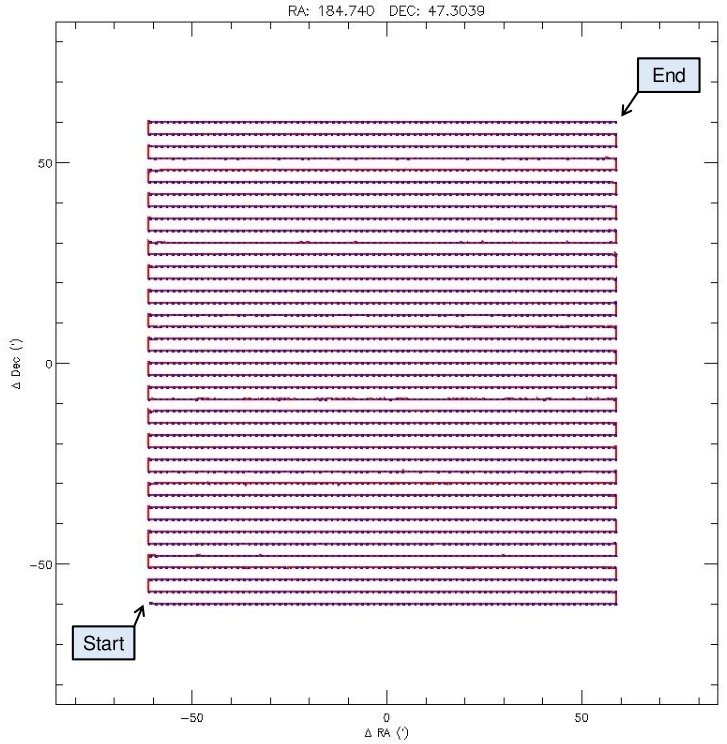
\includegraphics [width=0.6\linewidth] {RAlong.jpg}
\caption[RALongMap() GBT Antenna Trajectory]
{The actual GBT antenna trajectory (red) generated by executing script~\ref{lst:ralongmap}.
Blue dots mark timestamps of sampled data. (sampling frequency is set via
{\bf tint} in the configuration).
\label{fig:ralongmap}}
\end{center}
\end{figure}



%-----------------------------------------------------------------------------
\vspace{-0.5cm}
\subsubsection{RALongMapWithReference}

{\bfseries{\textcolor{pythonKeywords}{RALongMap}}} with periodic reference observations.

\vspace{-0.25cm}
\begin{description}[itemsep=1pt]
\item[{\bf SYNTAX}:]
{\bfseries{\textcolor{pythonKeywords}{RALongMapWithReference}}(}
location, hLength, vLength, vDelta, referenceOffset,\\ referenceInterval, scanDuration,
beamName, unidirectional, start, stop
{\bf)}
\item[Parameter Descriptions] See {\bfseries{\textcolor{pythonKeywords}{RALongMap}}}.
The following additional parameters are used to define the periodic reference
observations:
\begin{itemize}[itemsep=1pt]
\item {\bf referenceOffset}: An Offset object. It specifies the position of the 
reference source on the sky relative to the {\bf Location} specified by the first 
input parameter.
\item {\bf referenceInterval}: An integer. It specifies when to do a reference 
scan in terms of map rows.  For example, setting referenceInterval=4 will
periodically perform one scan on the reference source followed by 4 mapping scans.
\end{itemize}

\item[{\bf USAGE}:] Script~\ref{lst:ralongmapwithreference} produces a map with
6 rows each 60' long, using a row spacing of 6' and scan rate of 720'/min.
A reference position will be observed once before every 3 rows.  The sequence of
scans will be: reference $\rightarrow$ rows 1-3 $\rightarrow$
reference $\rightarrow$ rows 4-6.
\end{description}

\lstinputlisting[language=PythonAstrid,
backgroundcolor=\color{sbBackground},
caption={[RALongMapWithReference() example.]
RALongMapWithReference() example.},
label={lst:ralongmapwithreference}]
{ralongmapwithreference.py}

\newpage

%-----------------------------------------------------------------------------

\subsubsection{DecLatMap}

A Declination/Latitude map performs an \gls{OTF} raster scan centered
on a  sky location. Scans are performed in declination, latitude, or 
elevation coordinates depending on the desired coordinate system. The starting 
point of the map is defined as (-hLength/2, -vLength/2) from the specified
center location.

\begin{description}[itemsep=1pt]
\item[{\bf SYNTAX}:]
{\bfseries{\textcolor{pythonKeywords}{DecLatMap}}(}
location, hLength, vLength, hDelta, scanDuration, beamName,\\
unidirectional, start, stop
{\bf)}
\item[Parameter Descriptions] See {\bfseries{\textcolor{pythonKeywords}{RALongMap}}}
with the following difference:
\begin{itemize}[itemsep=1pt]
\item {\bf hDelta}: An Offset object. Similar to {\bf vDelta} in
{\bfseries{\textcolor{pythonKeywords}{RALongMap}}}. It specifies the horizontal
distance between map columns. {\bf hDelta} values must be positive.
\end{itemize}

\item[{\bf USAGE}:]
 Script~\ref{lst:declatmap} produces a map with 41 columns each
120' tall, using a column spacing of 3' and scan rate of 20'/min with beam 1 (default).
A plot showing the actual trajectory of the antenna on the sky when
script~\ref{lst:declatmap} was executed is shown in figure~\ref{fig:declatmap}.
Note that the blue dots in figure~\ref{fig:declatmap} mark timestamps
of the data sampled along the trajectory.

\end{description}

\lstinputlisting[language=PythonAstrid,
backgroundcolor=\color{sbBackground},
caption={[DecLatMap() example.]
DecLatMap() example.},
label={lst:declatmap}]
{declatmap.py}

\begin{figure}[!h]
\begin{center}
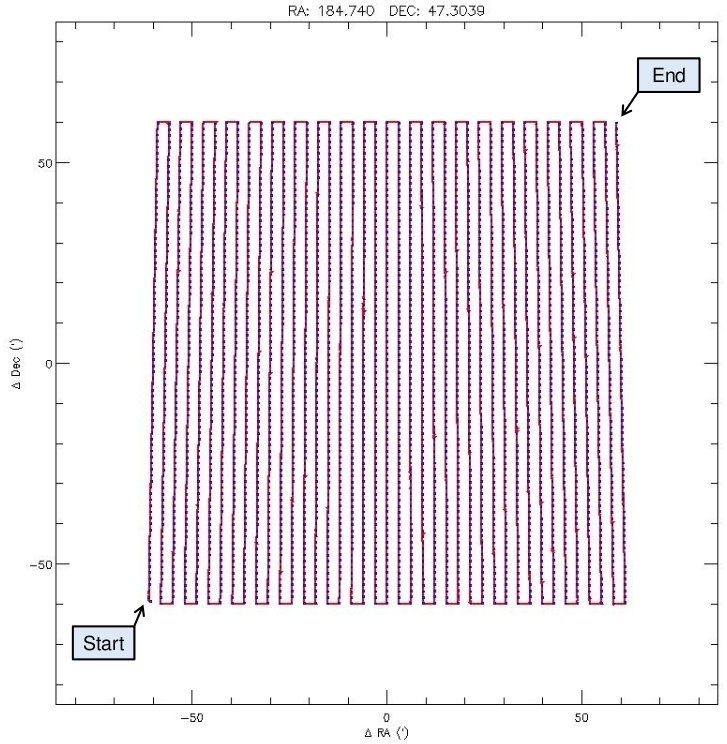
\includegraphics [width=0.6\linewidth] {DecLat.jpg}
\caption[DecLatMap() GBT Antenna Trajectory]
{The actual GBT antenna trajectory (red) generated by executing script~\ref{lst:declatmap}.
Blue dots mark timestamps of sampled data. (sampling frequency is set via
{\bf tint} in the configuration).
\label{fig:declatmap}}
\end{center}
\end{figure}


\newpage

%-----------------------------------------------------------------------------

\subsubsection{DecLatMapWithReference}

{\bfseries{\textcolor{pythonKeywords}{DecLatMap}}} with periodic reference observations.

\begin{description}[itemsep=0pt]
\item[{\bf SYNTAX}:]
{\bfseries{\textcolor{pythonKeywords}{DecLatMapWithReference}}(}
location, hLength, vLength, hDelta, referenceOffset,\\ referenceInterval, scanDuration,
beamName, unidirectional, start, stop
{\bf)}
\item[Parameter Descriptions] See {\bfseries{\textcolor{pythonKeywords}{RALongMap}}}
with the following difference:
\begin{itemize}[itemsep=0pt]
\item {\bf hDelta}: An Offset object. Similar to {\bf vDelta} in
{\bfseries{\textcolor{pythonKeywords}{RALongMap}}}. It specifies the horizontal
distance between map columns. {\bf hDelta} values must be positive.
\end{itemize}
The following parameters are used to define the periodic reference observations:
\begin{itemize}
\item {\bf referenceOffset} An Offset object. It specifies the position of the 
reference source on the sky relative to the {\bf Location} specified by the first 
input parameter.
\item {\bf referenceInterval} An integer. It specifies when to do a reference 
scan in terms of map columns.  For example, setting referenceInterval=4 will
periodically perform one scan on the reference source followed by 4 mapping scans.
\end{itemize}

\item[{\bf USAGE}:] Script~\ref{lst:declatmapwithreference} produces a map with
6 columns each 60' long, using a column spacing of 6' and scan rate of 720'/min.
A reference position will be observed once before every 3 columns.  The sequence of
scans will be: reference $\rightarrow$ columns 1-3 $\rightarrow$
reference $\rightarrow$ columns 4-6.
\end{description}

\lstinputlisting[language=PythonAstrid,
backgroundcolor=\color{sbBackground},
caption={[DecLatMapWithReference() example.]
DecLatMapWithReference() example.},
label={lst:declatmapwithreference}]
{declatmapwithreference.py}


%-----------------------------------------------------------------------------
\vspace{-5mm}
\subsubsection{PointMap}

A PointMap() constructs a map by sitting on fixed positions laid out on a grid.
The starting point of the map is defined as (-{\bf hlength}/2,-{\bf vLength}/2).

\begin{description}[itemsep=0pt]
\item[{\bf SYNTAX}:]\ \\
{\bfseries{\textcolor{pythonKeywords}{PointMap}}(}
location, hLength, vLength, hDelta, vDelta, scanDuration, beamName, start, stop
{\bf)}
\item[location] A Catalog source name or Location object. It specifies the 
center of the map.
\item[hLength] An Offset object. It specifies the horizontal width of the map. {\bf hLength} values
may be negative.
\item[vLength] An Offset object. It specifies the vertical height of the map. {\bf vLength} values
may be negative.
\item[hDelta] An Offset object. It specifies the horizontal distance between 
points in the map.  {\bf hDelta} values must be positive.
\item[vDelta] An Offset object. It specifies the vertical distance between 
points in the map. {\bf vDelta} values must be positive.
\item[scanDuration] A float. It specifies the length of each scan in seconds.
\item[beamName] A string. It specifies the receiver beam to use for the scan. 
{\bf beamName} can be \sq{C}, \sq{1}, \sq{2}, \sq{3}, \sq{4} or any valid combination
for the  receiver you are using such as \sq{MR12}. Default is \sq{1}.
\item[start] An integer. It specifies the starting point for the map. The 
default value for {\bf start} is 1.  Note in
{\bfseries{\textcolor{pythonKeywords}{PointMap}}} this counts points, not stripes.
\item[stop] An integer. It specifies the stopping point for the map. The 
default value for {\bf stop} is None, which means \dq{go to the end}.

\newpage

\item[{\bf USAGE}:]
Script~\ref{lst:pointmap} produces a 9 point map using a $3\times 3$ grid.  Points are
separated by 10 arc-seconds in RA and 10 arc-seconds in Dec.  Each point will
be observed for 30 seconds using beam 1 (default).  A plot showing the actual
trajectory of the antenna on the sky when script~\ref{lst:pointmap} was executed
is shown in figure~\ref{fig:pointmap}.  Note that the black crosses mark the
average positions of sampled data at each point.

\end{description}

\lstinputlisting[language=PythonAstrid,
backgroundcolor=\color{sbBackground},
caption={[PointMap() example.]
PointMap() example.},
label={lst:pointmap}]
{pointmap.py}

\begin{figure}[!h]
\begin{center}
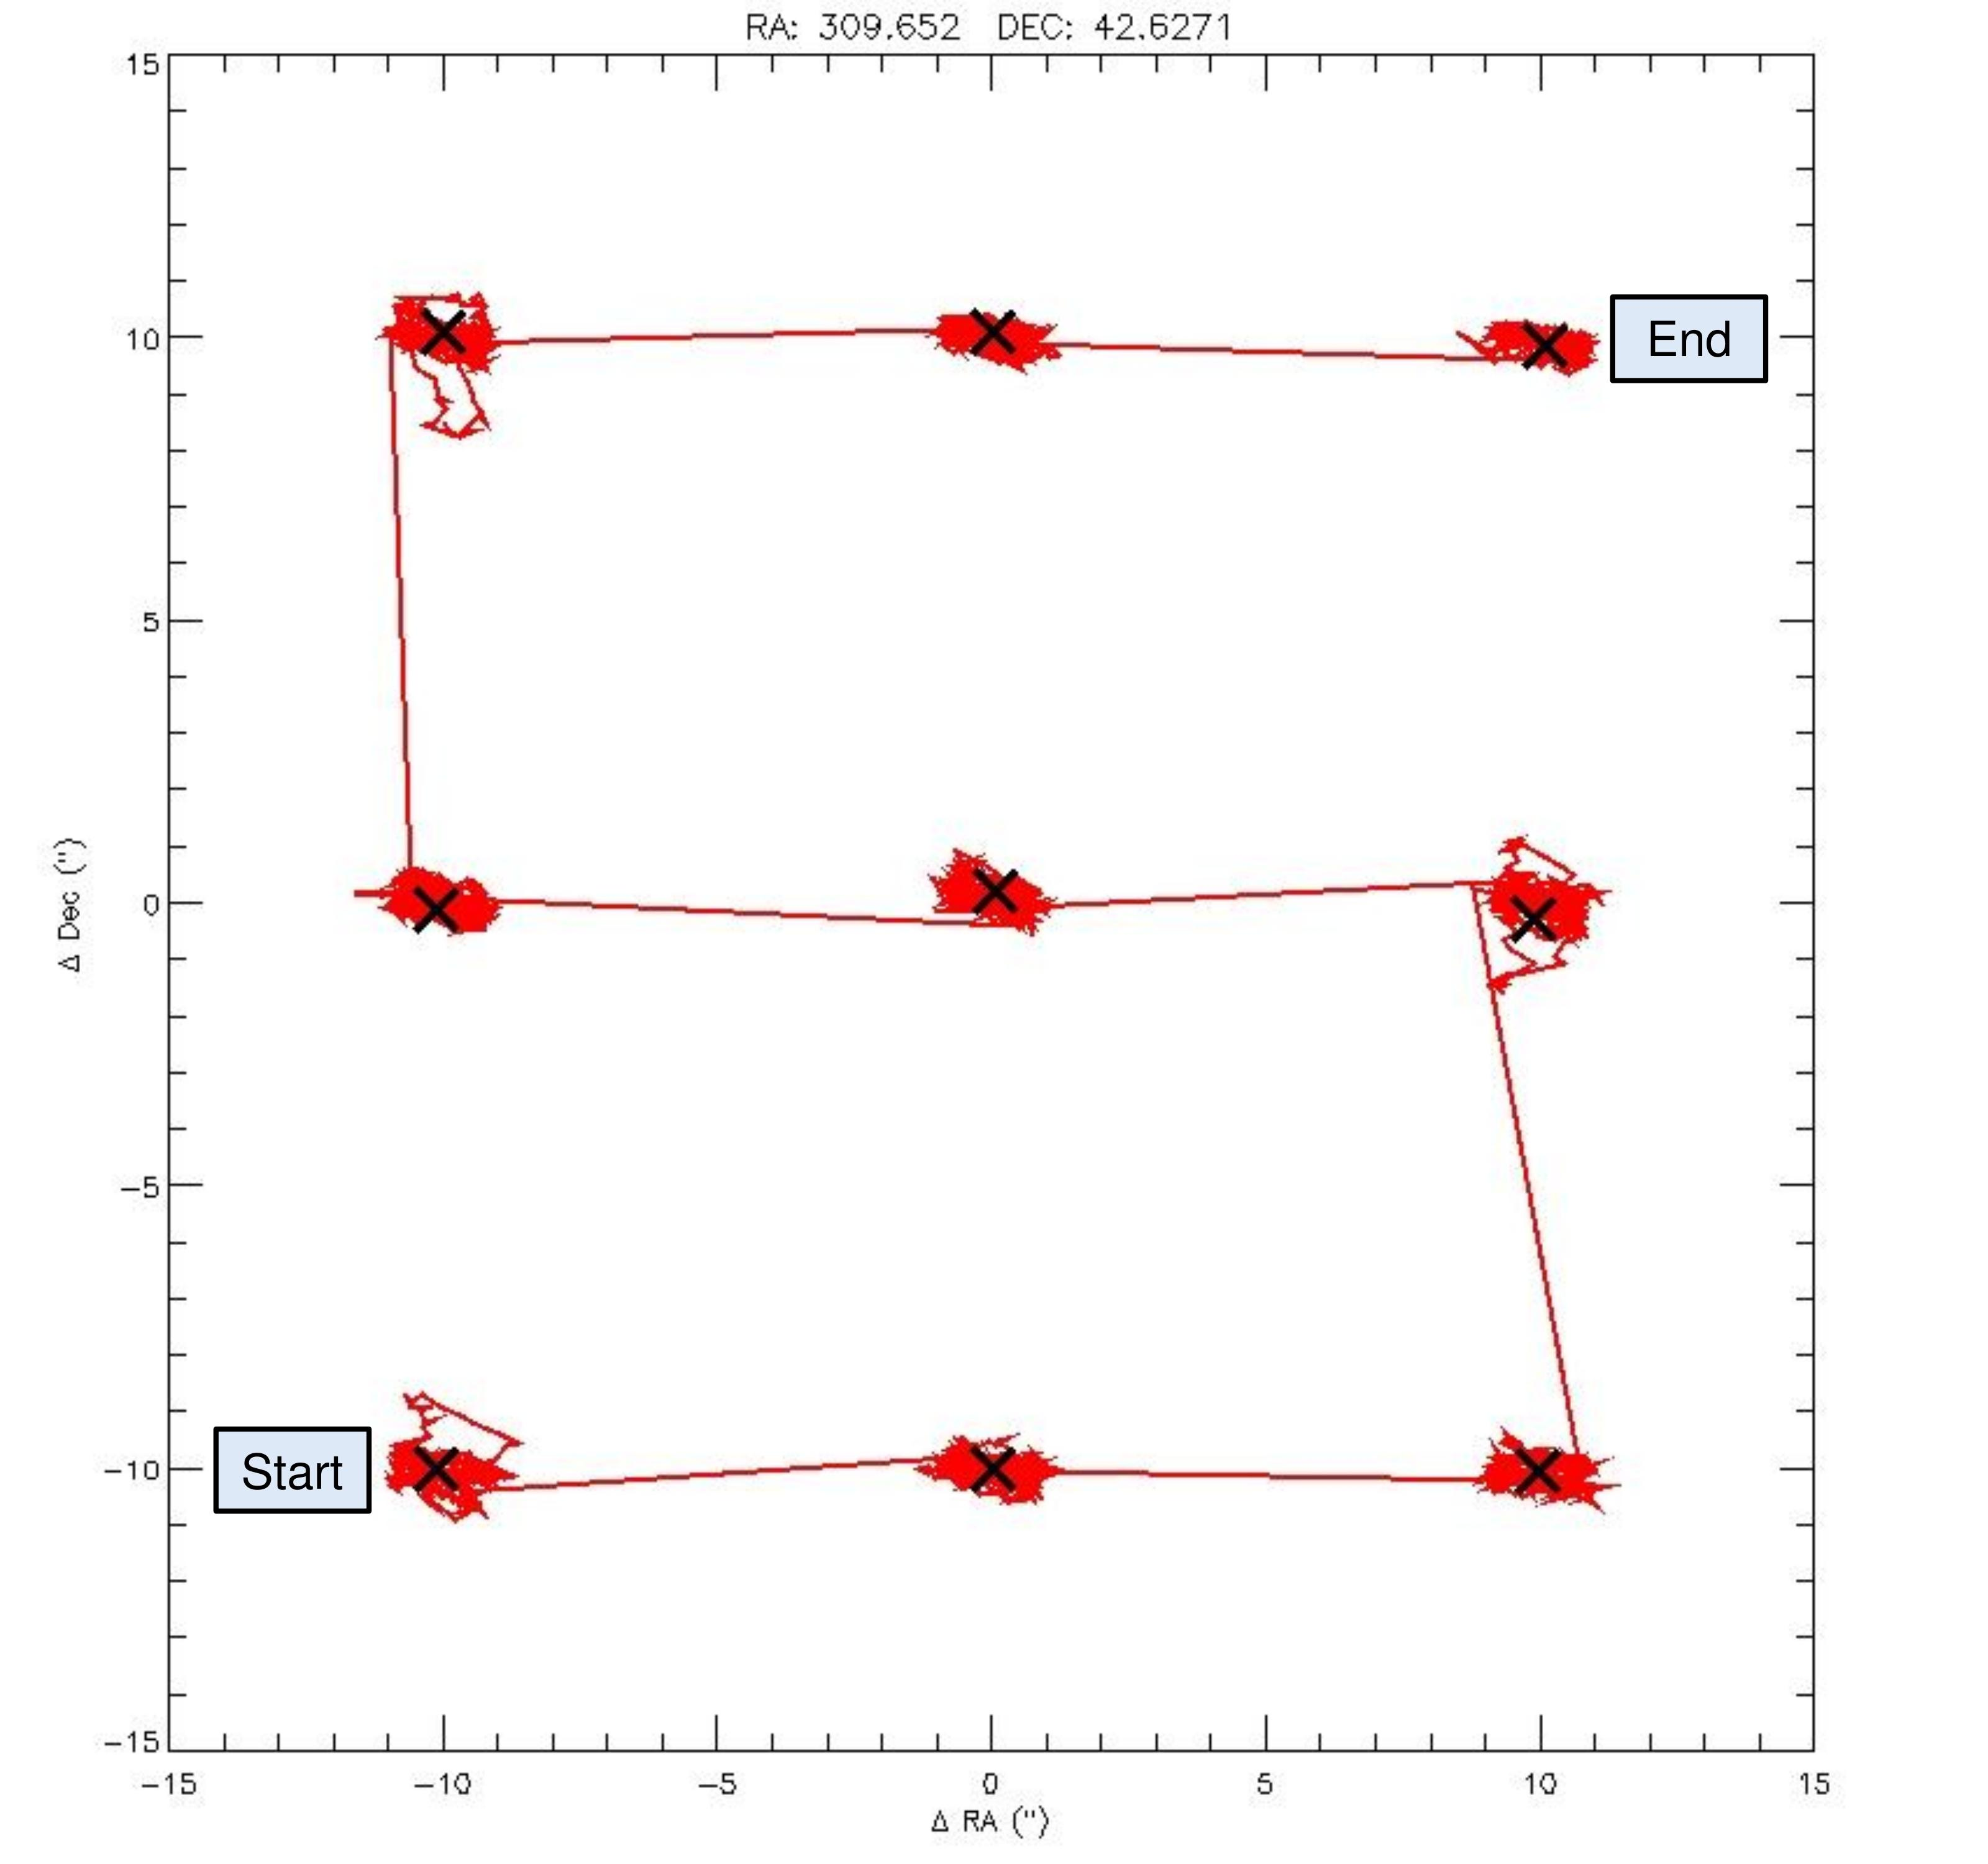
\includegraphics [width=0.85\linewidth] {pointmap.jpg}
\caption[PointMap() GBT Antenna Trajectory]
{A plot of the actual GBT antenna trajectory (red) generated by executing script~\ref{lst:pointmap}.
The average positions of data sampled at each point are marked with black crosses.
\label{fig:pointmap}}
\end{center}
\end{figure}


%-----------------------------------------------------------------------------
\newpage

\subsubsection{PointMapWithReference}

{\bfseries{\textcolor{pythonKeywords}{PointMap}}} with periodic reference observations.

\begin{description}
\item[{\bf SYNTAX}:]
{\bfseries{\textcolor{pythonKeywords}{PointMapWithReference}}(}
location, hLength, vLength, hDelta, vDelta, referenceOffset, referenceInterval,
scanDuration, beamName, start, stop
{\bf)}
\item[Parameter Descriptions] See {\bfseries{\textcolor{pythonKeywords}{PointMap}}}.
The following additional parameters are used to define the periodic reference
observations:
\begin{itemize}[itemsep=1pt]
\item {\bf referenceOffset}: An Offset object. It specifies the position of the 
reference source on the sky relative to the {\bf Location} specified by the first 
input parameter.
\item {\bf referenceInterval}: An integer. It specifies when to do a reference 
scan in terms of map points.  For example, setting referenceInterval=4 will
periodically perform one scan on the reference source followed by 4 pointed scans.
\end{itemize}

\item[{\bf USAGE}:] Script~\ref{lst:pointmapwithreference} produces a
$4\times 4$ point map using beam 1 (default).  A reference position will be
observed before every 2 points.  The sequence of scans will be:
reference(r) $\rightarrow $ points 1 and 2 ($P_{1,2}$)$\rightarrow r \rightarrow
P_{3,4} \rightarrow r \rightarrow P_{5,6} \rightarrow r \rightarrow P_{7,8}
\rightarrow r \rightarrow P_{9,10} \rightarrow r \rightarrow P_{11,12}
\rightarrow r \rightarrow P_{13,14} \rightarrow r \rightarrow P_{15,16}$.
\end{description}

\lstinputlisting[language=PythonAstrid,
backgroundcolor=\color{sbBackground},
caption={[PointMapWithReference() example.]
PointMapWithReference() example.},
label={lst:pointmapwithreference}]
{pointmapwithreference.py}





%-----------------------------------------------------------------------------

\subsubsection{Daisy}

The Daisy scan type performs an \gls{OTF} scan around a central point in the
form of daisy petals.  It is a useful observing mode for focal plance arrays,
allowing more integration time in the central field of view.

The {\bfseries{\textcolor{pythonKeywords}{Daisy}}} scan will produce an
approximately closed circular pattern on the sky after 22 radial oscillation
periods (see figure~\ref{fig:daisy22rad}). For beam-sizes of 20\arcsecond~\gls{FWHM}
or so, the circular area mapped will be fully sampled if the map radius is less
than 6\arcminute.  It is not an especially useful observing mode for
general-purpose single-beam mapping, since the largest \dq{hole} in the map
is $\sim 0.3\times$ the map radius.

\noindent Trajectories are generated according to:

\begin{align}
\Delta \hat{x}(t)& = \dfrac{r_{0}\sin(2\pi t / \tau+\phi_{1})
                            \cos(2t / \tau+\phi_{2})}
                           {\cos(\hat{y}_{0})}\label{eq:daisyx}\\[20pt]
\Delta \hat{y}(t)& = r_{0}\sin( 2\pi t / \tau+\phi_{1})
                     \sin(2t / \tau+\phi_{2})\label{eq:daisyy}
\end{align}

$\hat{x}$ and $\hat{y}$ are then major and minor coordinates of a sperical
coordinate system, $t$ is the time, $r_{0}$ is the map radius, $\tau$ is the radial
oscillation period, $\phi_{1}$ and $\phi_{2}$ are the radial and rotational phases,
and $\hat{y}_{0}$ is the minor coordinate of the map center.

\newpage

\begin{figure}[!h]
\begin{center}
\subfloat[Daisy scan with scanDuration = $5\times$radial\_osc\_period.
\label{fig:daisy5rad}]
{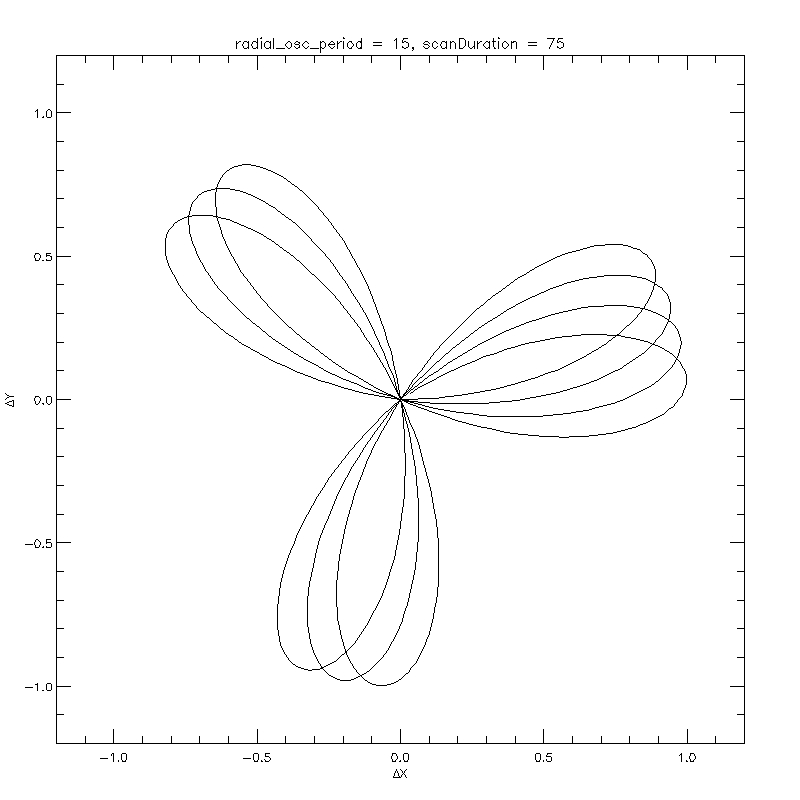
\includegraphics[width=.475\linewidth]{daisy5rad.jpg}}
\hfill
\subfloat[Daisy scan with scanDuration = $22\times$radial\_osc\_period.
\label{fig:daisy22rad}]
{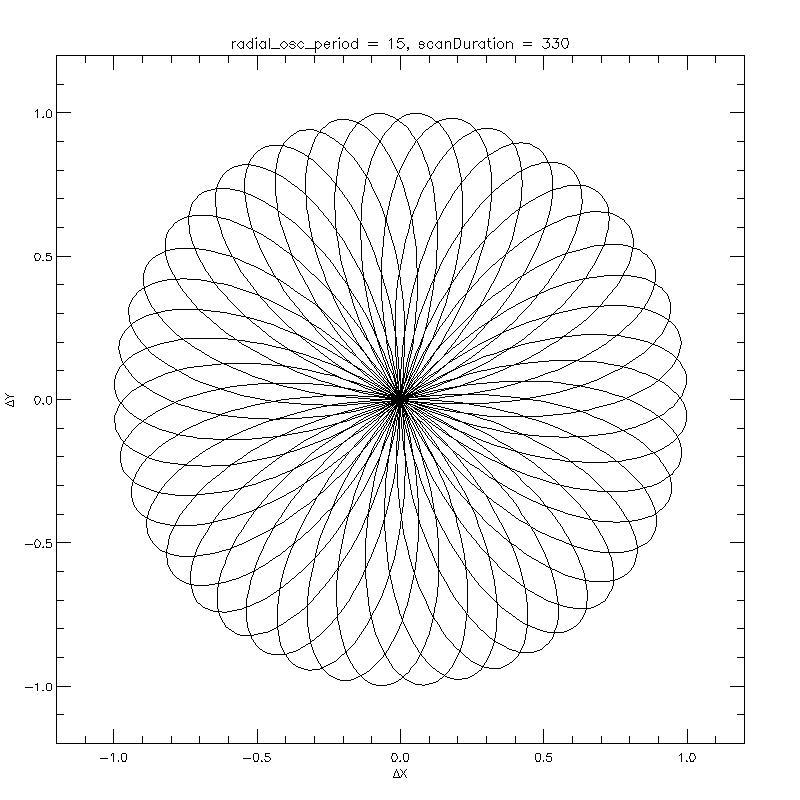
\includegraphics[width=.475\linewidth]{daisy22rad.jpg}}
\caption[Daisy map trajectory]
{Figure~\ref{fig:daisy5rad} shows the Daisy trajectory after 5 radial oscillations.
Figure~\ref{fig:daisy22rad} shows an approximately closed pattern after 22 radial
oscillations} 
\label{fig:daisytraj}
\end{center}
\end{figure}

\begin{description}
\item[{\bf SYNTAX}:]
{\bfseries{\textcolor{pythonKeywords}{Daisy}}(}
location, map\_radius, radial\_osc\_period, radial\_phase, rotation\_phase,\\
scanDuration, beamName, cos\_v, coordMode, calc\_dt
{\bf)}
\item[location] A Catalog source name or Location object. It specifies the 
center of the map.
\item[map\_radius] $r_{0}$ in equations~\ref{eq:daisyx} and~\ref{eq:daisyy}.
A float which specifies the radius of the map's \dq{daisy petals} in arc-minutes.
\item[radial\_osc\_period] $\tau$ in equations~\ref{eq:daisyx} and~\ref{eq:daisyy}.
A float which specifies the period of the radial oscillation in seconds.
\begin{itemize}
\item[{\bf --Note:}] not to be less than 15 sec $\times \sqrt{r_{0}/1.5\arcminute}$
for radii $>1.5\arcminute$ and in no case under 15 seconds.
\end{itemize}
\item[radial\_phase] $\phi_{1}$ in equations~\ref{eq:daisyx} and~\ref{eq:daisyy}.
A float which specifies the radial phase in radians.
\item[rotation\_phase] $\phi_{2}$ in equations~\ref{eq:daisyx} and~\ref{eq:daisyy}.
A float which specifies the rotational phase in radians.
\item[scanDuration] A float. It specifies the length of the scan in seconds.
\item[beamName] A string. It specifies the receiver beam to use for both 
scans. {\bf beamName} can be \sq{C}, \sq{1}, \sq{2}, \sq{3}, \sq{4} or any valid combination 
for the receiver you are using such as \sq{MR12}. The default value is \sq{1}.
\item[cos\_v] A Boolean. It specifies whether secant minor corrections (the
$\cos(\hat{y}_{0})$ term in equation~\ref{eq:daisyx}) should be used for the major axis
of the coordinate system.  The default is True.
\item[coordMode] A string. It specifies the coordinate mode for the radius that generate
the map. The default is \sq{AzEl}.
\item[calc\_dt] A float. It specifies time sampling used by the control system to calculate
a path.  Values should be between 0.1 and 0.5.  Calculating many points for a long daisy scan
can significantly increase overhead at scan startup.  The default is 0.1.

\item[{\bf USAGE}:] It takes approximately 22 radial oscillation periods to complete a
closed Daisy pattern.  However, {\bf radial\_oscillation\_period} is typically set to be in
the range of 15--60 seconds depending on the radius being used.  As an example, 22
ocillations of 20 seconds would take 440 seconds.  If a long trajectory such as this is
sent to the antenna manager, intrinsic inefficiencies in the array handling mechanism can
significantly increase overhead at the start of a scan.  Therefore one should try to
keep individual scans to 5 minutes or less.

Script~\ref{lst:daisy} will do 22 radial periods over 5 scans lasting 110 seconds each.
The {\bf rotation\_phase} and {\bf radial\_phase} arguments are used so that each scan
starts where the previous scan finished.  This will produce the closed Daisy pattern
shown in figure~\ref{fig:split_daisy}.  The entire \gls{SB} should take approximately
10 minutes to complete.
\end{description}

\lstinputlisting[language=PythonAstrid,
backgroundcolor=\color{sbBackground},
caption={[Daisy() example.]
Daisy() example.},
label={lst:daisy}]
{daisy.py}

\vspace{-0.5cm}

\begin{figure}[!h]
\begin{center}
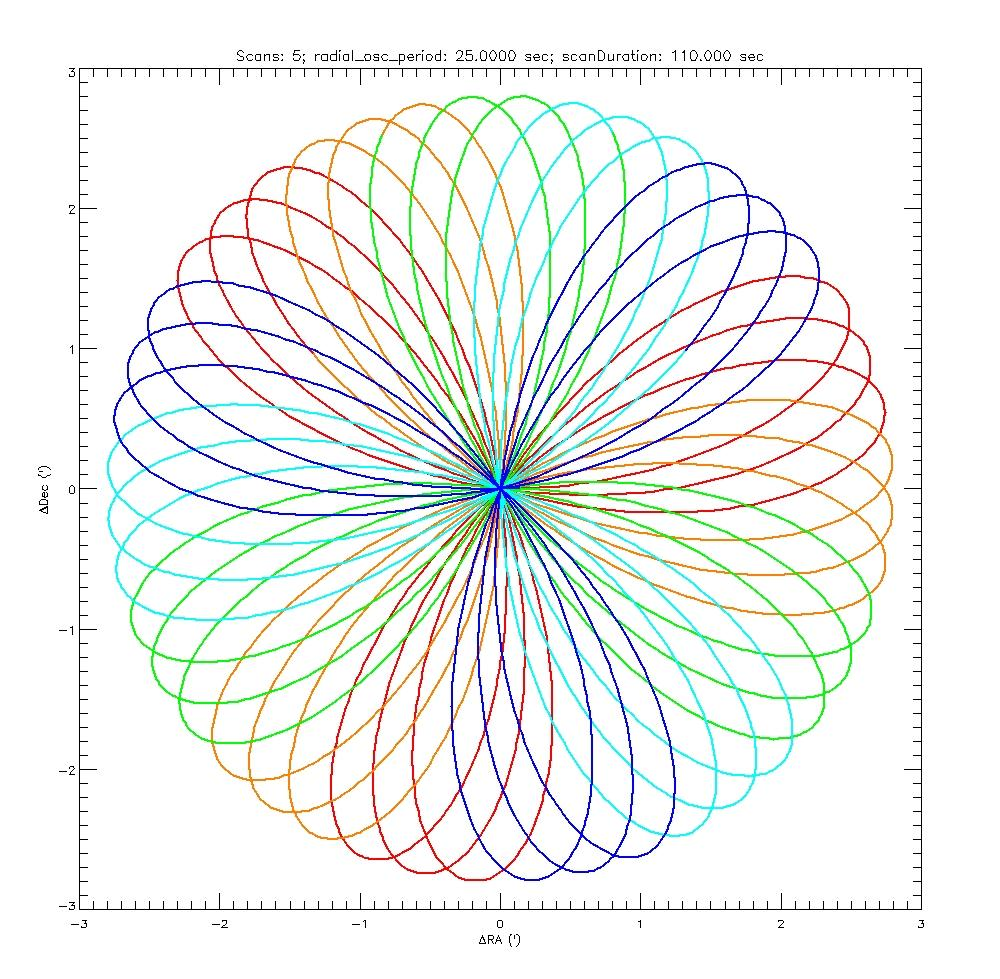
\includegraphics [width=0.65\linewidth] {split_daisy_exact.jpg}
\caption[Closed Daisy() GBT Antenna Trajectory split into multiple scans]
{A plot of the GBT antenna trajectory executed with script~\ref{lst:daisy}.
Each scan is plotted using a different color.
\label{fig:split_daisy}}
\end{center}
\end{figure}


\newpage



\section{Utility Functions}\label{sec:utility}

Utility functions are used in \glspl{SB} to control various aspects of
the \gls{GBT} other than data-taking scans.  This includes such things as
changing power levels, pausing the \gls{SB}, or waiting for a source to rise.
Please note that the syntax for all utility functions is case-sensitive.
Advanced utility functions are found in Appendix~\ref{appendix:advutil}.

%****************************************************************************
\subsection{Annotation}

The {\bfseries{\textcolor{pythonKeywords}{Annotation}}()} function allows you
to add any keyword and value to the \gls{GO} FITS file. This could be useful if
there is any  information you would like to record about your observation for later 
data processing, or for record keeping. Note that the information in a FITS KEYWORD
created via the {\bfseries{\textcolor{pythonKeywords}{Annotation}}()} function will
be ignored by the standard \gls{GBT} data reduction package \gls{GBTIDL}.  

\begin{description}[itemsep=1pt]
\item[{\bf SYNTAX}:]
{\bfseries{\textcolor{pythonKeywords}{Annotation}}(}
KEYWORD, Value
{\bf)}
\begin{description}[leftmargin=*]
\item[KEYWORD] A completely uppercase string of eight characters or less.  Do not
use any standard FITS keywords.
\item[Value] A string value for {\bf KEYWORD}.
\end{description}
\item[{\bf USAGE}:]
An example use of the {\bfseries{\textcolor{pythonKeywords}{Annotation}}()}
function is if you wish to specify what type of source you are observing.
Your sources might include H~II regions and Planetary Nebulae for example.
You could specify each type with
\end{description}

\lstinputlisting[language=PythonAstrid,
backgroundcolor=\color{sbBackground},
caption={[Annotation() example.]
Annotation() example.},
label={lst:annotation}]
{annotation.py}

%****************************************************************************
\subsection{Break}

The {\bfseries{\textcolor{pythonKeywords}{Break}}()} function inserts
a breakpoint into your \gls{SB} and gives the observer the choice of
continuing or terminating the \gls{SB}. When a breakpoint is encountered
during execution, your \gls{SB} is paused and a pop-up window is created.
The \gls{SB} remains paused for a set amount of time or until you acknowledge
the pop-up window and tell \gls{Astrid} to continue running your script.  

The {\bfseries{\textcolor{pythonKeywords}{Break}}()} function can take two
optional arguments, a message string and a timeout length.  Why have a timeout?
If an observer walks away from the control room during his or her observing
session (e.g. to go to lunch or the bathroom) and a breakpoint is reached,
it would be counterproductive to pause the observation indefinitely.
This will help save valuable telescope time.  

\begin{description}[itemsep=1pt]
\item[{\bf SYNTAX}:]
{\bfseries{\textcolor{pythonKeywords}{Break}}(}
message, timeout
{\bf)}
\begin{description}[leftmargin=*]
\item[message] A string.  Displayed in the pop-up dialog with a
default of \dq{Observation paused}
\item[timeout] A float. The number of seconds to get user-input before
continuing the \gls{SB}.  If you wish for the timeout to last forever then use
None.  The default is 300 seconds, or 5 minutes.
\end{description}
\item[{\bf USAGE}:]
\end{description}

\lstinputlisting[language=PythonAstrid,
backgroundcolor=\color{sbBackground},
caption={[Break() example.]
Break() example.},
label={lst:break}]
{break.py}


%****************************************************************************
\subsection{Comment}

The {\bfseries{\textcolor{pythonKeywords}{Comment}}()} function allows you
to add a comment into the \gls{Astrid} observing process which will be echoed
to the observation log during the observation. What's the difference between
this, and just writing comments with the pound (\#) sign in your \gls{SB}? 
When you use the pound sign to write your comments, they will not 
appear in the observation log when your \gls{SB} is run. Using the
{\bfseries{\textcolor{pythonKeywords}{Comment}}()} function directs your
comment to the output in the observation log. 

\begin{description}[itemsep=1pt]
\item[{\bf SYNTAX}:]
{\bfseries{\textcolor{pythonKeywords}{Comment}}(}
message
{\bf)}
\begin{description}[leftmargin=*]
\item[message] A string. Text to display during the observation.
\end{description}
\item[{\bf USAGE}:]
\end{description}

\lstinputlisting[language=PythonAstrid,
backgroundcolor=\color{sbBackground},
caption={[Comment() example.]
Comment() example.},
label={lst:comment}]
{comment.py}


%****************************************************************************
\subsection{GetUTC}

\begin{description}[itemsep=1pt]
\item[{\bf SYNTAX}:]
{\bfseries{\textcolor{pythonKeywords}{GetUTC}}()}
\begin{description}[leftmargin=*]
\item[Return Value:] A float. The current UTC time in decimal
hours since midnight.
\end{description}
\item[{\bf WARNING}:] If \gls{Astrid} is in \dq{offline} mode, then
{\bfseries{\textcolor{pythonKeywords}{GetUTC()}}} will return a value of None.
Attempting to validate Script~\ref{lst:getutc} without checking the return value
is not equal to None while \dq{offline} will result in an infinite loop.

\item[{\bf USAGE}:] The following example will repeatedly perform
{\bfseries{\textcolor{pythonKeywords}{Track}}} scans until the UTC time is past
12.0 hours.
\end{description}

\lstinputlisting[language=PythonAstrid,
backgroundcolor=\color{sbBackground},
caption={[GetUTC() example.]
GetUTC() example.},
label={lst:getutc}]
{getutc.py}


%****************************************************************************
\subsection{GetLST}

\begin{description}[itemsep=1pt]
\item[{\bf SYNTAX}:]
{\bfseries{\textcolor{pythonKeywords}{GetLST}}()}
\begin{description}[leftmargin=*]
\item[Return Value:] A float. The current Local Sidereal Time in
decimal hours.
\end{description}
\item[{\bf WARNING}:] If \gls{Astrid} is in \dq{offline} mode, then
{\bfseries{\textcolor{pythonKeywords}{GetLST()}}} will return a value of None.
Attempting to validate Script~\ref{lst:getlst} without checking the return value
is not equal to None while \dq{offline} will result in an infinite loop.
\item[{\bf USAGE}:] The following example will repeatedly perform
{\bfseries{\textcolor{pythonKeywords}{Track}}} scans on the source
\dq{1153+1107} until the LST is past 13.5 hours when the source \dq{1712+035} will
be observed once.
\end{description}

\lstinputlisting[language=PythonAstrid,
backgroundcolor=\color{sbBackground},
caption={[GetUTC() example.]
GetLST() example.},
label={lst:getlst}]
{getlst.py}


%****************************************************************************
\subsection{Now}

\begin{description}[itemsep=1pt]
\item[{\bf SYNTAX}:]
{\bfseries{\textcolor{pythonKeywords}{Now}}()}
\begin{description}[leftmargin=*]
\item[Return Value:] A UTC time object (see \S~\ref{sec:timeobject})
containing the UTC time and date.

\end{description}
\item[{\bf WARNING}:] If \gls{Astrid} is in \dq{offline} mode, then
{\bfseries{\textcolor{pythonKeywords}{Now}}()} will return a value of None.
Attempting to validate Script~\ref{lst:now} without checking the return value
is not equal to None while \dq{offline} will result in an infinite loop.

\item[{\bf USAGE}:] The following example will repeatedly perform
{\bfseries{\textcolor{pythonKeywords}{Track}}} scans on the source
\dq{1153+1107} until 09:54:12 UTC on 12 June 2016.
\end{description}

\lstinputlisting[language=PythonAstrid,
backgroundcolor=\color{sbBackground},
caption={[Now() example.]
Now() example.},
label={lst:now}]
{now.py}

%****************************************************************************
\subsection{WaitFor}

{\bfseries{\textcolor{pythonKeywords}{WaitFor}}()} pauses the \gls{SB}
until the specified time is reached.  The expected wait time is printed in
the observation log including a warning if the wait is longer than 10 minutes.
{\bfseries{\textcolor{pythonKeywords}{WaitFor}}()} will immediately return
if the specified time has already passed and is within the last 30 minutes. 
While {\bfseries{\textcolor{pythonKeywords}{WaitFor}}()} has the
\gls{SB} paused, it does not prevent the user from aborting.  However if the
user chooses to continue once the abort is detected, then the
{\bfseries{\textcolor{pythonKeywords}{WaitFor}}()} abandons the wait and
returns immediately.

\begin{description}[itemsep=1pt]
\item[{\bf SYNTAX}:]
{\bfseries{\textcolor{pythonKeywords}{WaitFor}}(}
Time\_object
{\bf)}
\begin{description}[leftmargin=*]
\item[Time\_object] A valid time object (see \S~\ref{sec:timeobject}).
\begin{itemize}
\item {\bf Note:} If a value of None is used as an argument to
{\bfseries{\textcolor{pythonKeywords}{WaitFor}}()}, the \gls{SB} will abort with
a message to the observation log.  This can occur when passing a value from
Horizon().GetRise() or Horizon().GetSet() when such an event may never occur,
such as the rise time for a circumpolar source.
\end{itemize}
\end{description}

\item[{\bf USAGE}:] The following example will pause the \gls{SB} until a
Local Sidereal Time of 15:13, then wait for the source \dq{1532\_3421} to rise
above $10^\circ$ elevation, and finally wait for the Sun to set below
$5^\circ$ elevation.
\end{description}

\lstinputlisting[language=PythonAstrid,
backgroundcolor=\color{sbBackground},
caption={[WaitFor() example.]
WaitFor() example.},
label={lst:waitfor}]
{waitfor.py}

%----------------------------------------------------

\subsection{ChangeAttenuation}

{\bfseries{\textcolor{pythonKeywords}{ChangeAttenuation}}()} allows the
observer to change all the attenuators in the IF Rack or the Converter Rack
by the same ammount.

\begin{description}[itemsep=1pt]
\item[{\bf SYNTAX}:]
{\bfseries{\textcolor{pythonKeywords}{ChangeAttenuation}}(}
devicename, attnchange
{\bf)}
\begin{description}[leftmargin=*]
\item[devicename] A string that can be either \sq{IFRack} or \sq{ConverterRack}.
This specifies the device in which the attenuators will be changed.
\item[attnchange] A float. This specifies how much the attenuators should 
be changed. This value can be either positive or negative.  
\begin{itemize}
\item {\bf Note:} if any new attenuator setting is less than zero or exceeds
the maximum value, 31 for the IF Rack and 31.875 for the Converter Rack, then the 
attenuator settings is made to be the appropriate limiting value.
\end{itemize}
\end{description}

\item[{\bf USAGE}:] The Following example adds 1 to the attenuation value in the
IF rack and subtracts 0.5 from the attenuation value in the converter rack.
\end{description}

\lstinputlisting[language=PythonAstrid,
backgroundcolor=\color{sbBackground},
caption={[ChangeAttenuation() example.]
ChangeAttenuation() example.},
label={lst:changeattenuation}]
{changeattenuation.py}

\newpage

%============================================================================
\section{Scheduling Block Objects}\label{sec:objects}

\glsuseri{SB} Objects are Python objects that are used to contain multiple pieces
of information within a single variable.  These are used with positions (requiring
a major and minor axis value along with an epoch), times (requiring the date and
the time of day), and for defining a horizon for the minimum elevation below which
you would not want to observe.

%****************************************************************************
\subsection{Location Object}\label{sec:location_objects}

A Location object is used to represent a particular location on the sky.

\begin{description}[itemsep=1pt]
\item[{\bf SYNTAX}:]
{\bfseries{\textcolor{pythonKeywords}{Location}}(}
coordinateMode, value1, value2
{\bf)}
\item[coordinateMode] A string.  The following modes are allowed:
\sq{J2000}, \sq{B1950}, \sq{RaDecOfDate}, \sq{HaDec}, \sq{ApparentRaDec},
\sq{Galactic}, \sq{AzEl}, and \sq{Encoder}
\item[value1, value2] May be a float, or sexagesimal quoted as a string (i.e.
\sq{hh:mm:ss.s}).  A location must be specified by these two values, the
meanings of  which are dependent on the both the chosen coordinate mode and
value type of each unit:
\begin{itemize}
\item {\bf float values}: will always denote units in degrees of arc, regardless
of the coordinate mode.
\begin{itemize}
\item This should not be confused with decimal use in Catalogs
(see \S~\ref{sec:catalogs}) which denote decimal hours for RA and HA, and
degrees of arc for all other angles.
\end{itemize}
\item {\bf sexagesimal value1}: Represent units of time for J2000, B1950, ApparentRaDec,
and RaDecOfDate and degrees of arc for HaDec, Galactic, AzEl and Encoder.
\item {\bf sexagesimal value2}: Represent degrees of arc.
\end{itemize}
\item[{\bf USAGE}:]
\end{description}

\lstinputlisting[language=PythonAstrid,
backgroundcolor=\color{sbBackground},
caption={[Specifying Location Objects.]
Specifying Location Objects.},
label={lst:location}]
{location.py}

\newpage

%****************************************************************************
\subsection{Offset Object}\label{sec:offset_objects}
An Offset is a displacement from the position of a source or from the
center position of a map.  Offset objects may be added to other offset objects
with the same coordinate mode and cosv correction. Offset objects may be added to
Location objects with the same coordinate mode.  {\bf Note that such addition is
not commutative and must be of the form}
({\bfseries{\textcolor{pythonKeywords}{Location}}}+{\bfseries{\textcolor{pythonKeywords}{Offset}}}).
{\bfseries{\textcolor{pythonKeywords}{Offset}}}+{\bfseries{\textcolor{pythonKeywords}{Location}}}
will produce a validation error.

\begin{description}[itemsep=1pt]
\item[{\bf SYNTAX}:]
{\bfseries{\textcolor{pythonKeywords}{Offset}}(}
coordinateMode, value1, value2, cosv
{\bf)}
\item[coordinateMode] A string.  The following modes are allowed:
\sq{J2000}, \sq{B1950}, \sq{RaDecOfDate}, \sq{HaDec}, \sq{ApparentRaDec},
\sq{Galactic}, \sq{AzEl}, and \sq{Encoder}
\item[value1, value2] May be a float, or sexagesimal quoted as a string (i.e.
\sq{hh:mm:ss.s}).  An offset must be specified by these two values, the meanings of
which are dependent on the both the chosen coordinate mode and value type of each unit:
\begin{itemize}
\item {\bf float values}: will always denote units in degrees of arc, regardless
of the coordinate mode.
\begin{itemize}
\item This should not be confused with decimal use in Catalogs
(see \S~\ref{sec:catalogs}) which denote decimal hours for RA and HA, and
degrees of arc for all other angles.
\end{itemize}
\item {\bf sexagesimal value1}: Represent units of time for J2000, B1950, ApparentRaDec,
and RaDecOfDate and degrees of arc for HaDec, Galactic, AzEl and Encoder.
\item {\bf sexagesimal value2}: Represent degrees of arc.
\end{itemize}
\item[cosv] A Boolean. It specifies whether secant minor corrections in
equation~\ref{eq:cosv} should be used for the major axis of the coordinate system
(i.e. $h/\cos(v)$ is the offset value in the direction of $h$).  The default is
True.  Since coordinate distances and angular separations are not equivalent for
sperical coordinate systems, the following approximations may be used for small
separations:

\vspace{-0.5cm}
\begin{align}
\Delta v& = v_{1} - v_{2} \\
\Delta h & = (h_1 - h_2)\cdot cos(v)
\label{eq:cosv}
\end{align}

where $h$ is the value of the major coordinate axis and $v$ is the value of the minor
coordinate axis.  For example, setting cosv=True with J2000 coordinate offsets will apply a
$\cos(Dec)$ term from equation~\ref{eq:cosv} to make maps appear rectangular if plotted
with $\Delta RA$ vs. $\Delta Dec$ relative to a central location.

\item[{\bf USAGE}:] Script~\ref{lst:offset} gives examples of adding Offset objects to
Location and other Offset objects.  The resulting coordinates are printed to screen.
\end{description}

\lstinputlisting[language=PythonAstrid,
backgroundcolor=\color{sbBackground},
caption={[Adding Offset Objects.]
Adding Offset objects to Location objects and other Offset objects.},
label={lst:offset}]
{offset.py}

%****************************************************************************

\subsection{Horizon Object}\label{sec:horizonobject}

Observing Scripts allow an observer to specify a definition of the horizon.
The user defined horizon can be used to begin an observation when an object 
\dq{rises} and/or end the observation when it \dq{sets} relative to the 
specified elevation of the \dq{horizon}. The Horizon object may be used 
to obtain the initial time that a given source is above the specified horizon 
(including an approximate atmospheric refraction correction).

\begin{description}
\item[{\bf SYNTAX}:]\ \\
{\bfseries{\textcolor{pythonKeywords}{Horizon}}(}
elevation
{\bf)}\ \\
\item[{\bf FUNCTIONS}:]\ \\
{\bfseries{\textcolor{pythonKeywords}{Horizon}}(}
elevation
{\bf).}{\bfseries{\textcolor{pythonKeywords}{GetRise}}(}
location {\bf )}\\
{\bfseries{\textcolor{pythonKeywords}{Horizon}}(}
elevation
{\bf).}{\bfseries{\textcolor{pythonKeywords}{GetSet}}(}
location {\bf )}
\item[location] A Catalog source name or Location object using a spherical coordinate
mode.  {\bfseries{\textcolor{pythonKeywords}{Horizon}}()} will not work with planets
and ephemeris tables.
\item[elevation] A float.  The Horizon elevation in degrees.  The default is 5.25 (the
nominal \gls{GBT} horizon limit).
\item[Return Value:] A UTC time object (see \S~\ref{sec:timeobject}) containing the UTC
time and date.
\begin{itemize}
\item {\bfseries{\textcolor{pythonKeywords}{GetRise}}(}source{\bf)} will return
the most recent rise time if the source is currently above the horizon, or the next rise
time if the source has not yet risen.
{\bfseries{\textcolor{pythonKeywords}{GetRise}}(}source{\bf)} will return {\bf None} if
the source never rises and the current time if the source never sets.

\item {\bfseries{\textcolor{pythonKeywords}{GetSet}}(}source{\bf)} will return the
next set time of the source.
{\bfseries{\textcolor{pythonKeywords}{GetSet}}(}source{\bf)} will return {\bf None} if
the source never sets and the current time if the source never rises.
\end{itemize}

\end{description}

\begin{description}
\item[{\bf USAGE}:]
Any Horizon object may be substituted as a start or stop time in scan types, such
as {\bfseries{\textcolor{pythonKeywords}{Track}}()}.  Script~\ref{lst:horizon} will
display the time when VirgoA rises above $20^\circ$ elevation.  Depending on the position
of the source at the time of execution, the \gls{SB} would then either begin a
{\bfseries{\textcolor{pythonKeywords}{Track}}()} scan immediately or
wait for VirgoA to rise above $5.25^\circ$ elevation before beginning the scan.
In both cases, the \gls{SB} would terminate the next time VirgoA sets below
$5.25^\circ$ elevation.
\end{description}

\lstinputlisting[language=PythonAstrid,
backgroundcolor=\color{sbBackground},
caption={[Horizon Objects.]
Using Horizon Objects.},
label={lst:horizon}]
{horizon.py}


%****************************************************************************
\newpage
\subsection{Time Object}\label{sec:timeobject}

The Time Object is primarily used for defining scan start or stop times.
The time may be represented as either a sexegesimal string or in a python
mxDateTime object.  You can learn more about mxDateTime at
\htmladdnormallink{http://www.egenix.com/files/python/mxDateTime.html}
{http://www.egenix.com/files/python/mxDateTime.html}
\footnote{ Note, one must access the python DateTime module directly 
from an observation script to generate time objects, i.e., using 
mx import DateTime.}.

\begin{description}
\item[{\bf SYNTAX}:]\ \\
\end{description} \vspace{-0.5cm}
The Time Object can be expressed in either UTC or LST.  The time can
be either absolute or relative.  An absolute or dated time specifies both 
the time of day and the date. An absolute time may be represented by either 
a sexegesimal string, i.e., \dq{yyyy-mm-dd hh:mm:ss} or by a DateTime object.
Relative or dateless times are specified by the time of day for \dq{today}.
\dq{WaitFor} will treat a dateless time that is more than 30 minutes in the past
as being in the future, i.e., the next day. Relative times may be represented
by either a sexegesimal string, i.e., \dq{hh:mm:ss} or a DateTimeDelta object.

For UTC times, the sexegesimal representation may include a \dq{UTC} suffix. 
Note that mxDateTime objects are always UTC. LST time may only be used with
relative times and the sexegesimal representation must include a \dq{LST} suffix.

Time Objects can have slightly varying formats and can be created in
a few different ways.  Some examples are:
\begin{description}

\item[\dq{2006-03-22 15:34:10}] Absolute time in UTC represented by a string.

\item[DateTime.TimeDelta(12, 0, 0)] Relative time in UTC as a mxDateTime 
object.

\item[\dq{2006/03/22 15:34:10 UTC}]  Absolute time in UTC represented by a string.

\item[\dq{22:15:48 LST}] Relative time in LST as a string.

\item[DateTime.DateTime(2006, 1, 21, 3, 45, 0)] Absolute time in UTC as a 
mxDateTime object.

\end{description}

\begin{description}
\item[{\bf USAGE}:] In this example we will continue to do one minute observations of srcA
until  Feb 12, 2007 at 13:15 UTC when we will then do a ten minute observations of srcB.
\end{description}

\lstinputlisting[language=PythonAstrid,
backgroundcolor=\color{sbBackground},
caption={[Time Objects.]
Using Time Objects.},
label={lst:time}]
{time_object.py}


%============================================================================
\newpage
%herez
\section{Example Scheduling Blocks}\label{sec:sbexamples}

For the following \gls{SB} examples we will use the configuration examples from
\S~\ref{sec:config}.  All configurations, catalogs and scripts are available within the
Green Bank computing environment at
\begin{verbatim}
/home/astro-util/projects/GBTog/
\end{verbatim}

\noindent The following catalog (sources.cat) will be used for all examples:

\lstinputlisting[language=PythonAstrid,
caption={[The catalog used with SB examples]The {\tt sources.cat} catalog used for the
\gls{SB} examples in this section.},
backgroundcolor=\color{catalogBackground}]
{sources.cat}

%****************************************************************************
\subsection[Frequency Switched Observations Looping Through a List of Sources]
{Frequency Switched Observations Looping Through a List of Sources}

In this example we perform frequency switched observations of the HI 21~cm
line towards several different sources.\\ \\
This example is available as {\tt/home/astro-util/projects/GBTog/SBs/example1.py}.

\lstinputlisting[language=PythonAstrid,
backgroundcolor=\color{sbBackground},
caption={[SB example 1 -- Frequency switched observations looping through a list
of sources.]
SB Example 1 -- Frequency switched observations looping through a list of sources.},
label={lst:sb_example1}]
{example1.py}

%****************************************************************************
\newpage
\subsection[Position Switched Observations Repeatedly Observing the Same Source]
{Position Switched Observations Repeatedly Observing the Same Source}

In this example we perform position switched observations of a single source.
We observe the source for two minutes and the off position for two minutes.
This is repeated twenty times.\\ \\
This example is available as {\tt/home/astro-util/projects/GBTog/SBs/example2.py}.

\lstinputlisting[language=PythonAstrid,
backgroundcolor=\color{sbBackground},
caption={[SB example 2 -- Position switched observations repeatedly observing
the same source.]
SB Example 2 -- Position switched observations repeatedly observing the same source.},
label={lst:sb_example2}]
{example2.py}


%****************************************************************************
\newpage
\subsection[Position Switched Observations of Several Sources and Using
the Horizon Object]
{Position Switched Observations of Several Sources and Using
the Horizon Object}

In this example we perform position switched observations of three sources.
We observe the first source until the second source rises above $20^\circ$ elevation.
Then we observe the second source until it goes below $20^\circ$ elevation at which
point we observe a third source.\\ \\
This example is available as {\tt/home/astro-util/projects/GBTog/SBs/example3.py}.

\lstinputlisting[language=PythonAstrid,
backgroundcolor=\color{sbBackground},
caption={[SB example 3 -- Position switched observations of several sources
using Horizon().]
SB Example 3 -- Position switched observations of several sources and using the
Horizon object.},
label={lst:sb_example3}]
{example3.py}

%****************************************************************************
\newpage
\subsection{Frequency Switched On-The-Fly Mapping}

In this example we perform frequency switched observations of the HI 21~cm
line to map a $5\times5$ degree region of the sky.  We use pixels that are
3\arcminute\ in size and have an integration time of 2 seconds per pixel.
We do not observe the whole map in this example. \\
\\
This example is available as {\tt/home/astro-util/projects/GBTog/SBs/example4.py}.

\lstinputlisting[language=PythonAstrid,
backgroundcolor=\color{sbBackground},
caption={[SB example 4 -- Frequency switched On-The-Fly mapping.]
SB Example 3 -- Frequency switched On-The-Fly mapping.},
label={lst:sb_example4}]
{example4.py}


%****************************************************************************
\newpage

\section{What Makes a Good Scheduling Block}

Rarely does an observing session exactly follow one's plans.  A useful
philosophy is to consider the work that would be involved in editing
an \gls{SB} if something were to go wrong during its execution
and you wanted to resume its execution where you left off.
You should break apart any long scripts into smaller individual scripts
to reduce the need for edits.  

During your observing, you will make decisions as to how to proceed
with the next observations.  You should break apart large scripts to increase
your flexibility in being able to react to the circurmstances that
arise during your observing.

We recommend that the following should be avoided within a single \gls{SB}, as
it will make the block too long:
\begin{itemize}
\item {\bf Multiple Configurations}: Multiple configurations (peak/focus and
science observations should optimally be perfomed with separate \glspl{SB}.
\item {\bf Changing Receivers}: You should only use a single receiver within
an \gls{SB}.
\item {\bf Multiple Maps}: You should perform only a single map within any
\gls{SB}.
\end{itemize}










%%%%%%%%%%%%%%%%%%%%%%%%% END CHAPTER %%%%%%%%%%%%%%%%%%%%%%%




%\begin{table}
%\centering
%\begin{threeparttable}
%\scriptsize
%\caption[]{VEGAS observing modes and the relevant astrid keywords} \label{tab:vegas_modes}
%\begin{tabular}{|l|r|r|r|r|r|} \hline
%Mode & Bandwidth  & Number of  & Spectral   &  nchan        &    vegas.subband\tnote{a}     \\
%     &            & Channels   & Resolution &               &                     \\
%     &            &            &            &               &                      \\
%     & (MHz)      &            & (KHz)      &               &                       \\                 \hline
%\multicolumn{6}{|c|}{Single Spectral Window Modes\tnote{b}}                     \\ \hline
%1   & 1500\tnote{c} & 1024        & 1465       & low        &    N/A  \\
%2   & 1500\tnote{c} & 16384       & 92         & high       &    N/A  \\
%3   & 1080\tnote{d} & 16384       & 66         & high       &    N/A  \\
%4   & 187.5      & 32768       & 5.7        & low           &    N/A  \\
%5   & 187.5      & 65536       & 2.9        & medium        &    N/A  \\
%6   & 187.5      & 131072      & 1.4        & high          &    N/A  \\
%7   & 100        & 32768       & 3.1        & low           &    N/A  \\
%8   & 100        & 65536       & 1.5        & medium        &    N/A  \\
%9   & 100        & 131072        & 0.8      & high          &    N/A  \\
%10  & 23.44      & 32768         & 0.7      & low           &    1    \\
%11  & 23.44      & 65536         & 0.4      & medium-low    &    1    \\
%12  & 23.44      & 131072        & 0.2      & medium        &    1    \\
%13  & 23.44      & 262144        & 0.1      & medium-high   &    1    \\
%14  & 23.44      & 524288        & 0.05      & high         &    N/A  \\
%15  & 11.72      & 32768         & 0.4       & low          &    N/A  \\
%16  & 11.72      & 65536         & 0.2       & medium-low   &    N/A  \\
%17  & 11.72      & 131072        & 0.1       & medium       &    N/A  \\
%18  & 11.72      & 262144        & 0.05      & medium-high  &    N/A  \\
%19  & 11.72      & 524288        & 0.02      & high         &    N/A  \\ \hline
%\multicolumn{6}{|c|}{Eight Spectral Window Modes\tnote{e}} \\ \hline
%20 & 23.44      & 4096          & 5.7        & low          &   8  \\
%21 & 23.44      & 8192          & 2.9        & medium-low   &   8 \\ 
%22 & 23.44      & 16384          & 1.4       & medium       &   8 \\
%23 & 23.44      & 32768         & 0.7        & medium-high  &   8 \\
%24 & 23.44      & 65536         & 0.4        & high         &   8  \\
%25 & 16.9      & 4096          & 4.1       & low          &   N/A \\
%26 & 16.9      & 8192          & 2.1       & medium-low   &   N/A \\
%27 & 16.9      & 16384         & 1.0      & medium       &   N/A \\
%28 & 16.9      & 32768         & 0.5      & medium-high  &   N/A \\
%29 & 16.9      & 65536         & 0.26      & high         &   N/A \\ \hline
%\end{tabular}
%\begin{tablenotes}
%\item [a] This configuration parameter is required to tell the single
%  spectral window 23.44 MHz mode from the eight spectral window 23.44
%  MHz mode.
%\item [b] These modes provide one spectral window per spectrometer.
%\item [c] The useable bandwidth for this mode is 1250~MHz.
%\item [d] The useable bandwidth for this mode is 850~MHz.
%\item [e] These modes provide up to eight spectral windows per
%  spectrometer. For modes 20-24, the spectral windows must be placed
%  within 1500~MHz with a useable frequency range of 150 to
%  1400~MHz. For modes 25-29, the spectral windows must be placed
%  within 1000~MHz with a useable frequency range of 150 to 950~MHz.
%\end{tablenotes}
%\end{threeparttable}
%\end{table}
%\latex{\end{landscape}}


%Default values are listed in Table~\ref{table:iftarget}.
%%This needs updating for VEGAS
%\begin{table}[!h]
%\begin{center}
%\caption[IF target levels]{The default \IF\ target levels.  
% Configurations using the \gls{spigot} will 
% be set to the \glsunset{ACS}\ACS\ 
% target levels specified in the table. 
%The receiver categories A, B, and C are actually based on the 
%nominal \IF\ center frequencies 
%for these receivers (3, 6 and 1.08 GHz, respectively). 
%The Receiver Groups are as follows: 
%A) \gls{Lband}, \gls{Cband}, \gls{Xband}, \gls{Kuband}; 
%B) \gls{Sband}, \gls{KFPA}, \gls{Kaband}, \gls{Qband}; 
%and C) any prime focus receiver (\gls{Pband}). The \IF\ target levels for VEGAS are still being determined.
%\label{table:iftarget}}
%\begin{tabular}{|l|l|l|l|l|l|}
%\hline
%Receiver & \gls{IFRack} & \multicolumn{2}{|c|}{ \glsunset{ACS}\ACS\ 50 \& 12.5 MHz} & \glsunset{ACS}\ACS\ 800 MHz & All Other \\
%Group & Bandwidth & 9 Level & 3 Level & \& 200 MHz & backends \\ 
% & (MHz) & (Volts) & (Volts) & (Volts) & (Volts) \\
%\hline
%A &      20  &	0.1  &	0.5  &	1.0  & 1.0  \\
%A &      80  &	0.1  &	0.5  &	1.0  &	1.0  \\
%A &      320  &	1.0  &	1.0  &	1.0  &	1.0  \\
%A &      1280  &	1.0  &	1.0  &	1.0  &	1.0  \\
%B &      80  &	1.0  &	1.0  &	1.0  &	1.0  \\
%B &      320  &	1.0  &	1.0  &	1.0  &	1.0  \\
%B &      1280  &	1.0  &	1.0  &	1.0  &	1.0  \\
%A or B & AllPass &	3.0  &	5.0  &	1.0  &	1.0  \\
%C &      $\leq 80$ &	0.1  &	0.5  &	1.0  &	1.0  \\
%C &      $> 80$ &	1.0  &	1.0  &	1.0  &	1.0  \\
%\hline
%\end{tabular}
%\end{center}
%\end{table}


%%%%%%%%%%%%%%%%something is wrong with vred calculations %%%%%%%%%%%%%%%%%%%%%%%
%\item[{\bf \large vlow} and {\bf \large vhigh}] These keywords specify the minimum 
%and maximum velocity or
%value of Z (if vdef=\dq{Red}) to be observed from a group of sources.
%The value is a float and is in ${\rm km~s^{-1}}$ for velocities.  The 
%default value is 0.0.  See Appendix~\ref{appendix:vlowhigh} for more details on the
%use of vlow and vhigh.  The use of vlow and vhigh is not recommended for frequencies where there
%can be large amounts of \RFI.

% \item[{\bf \large sp.mode}] This keyword specifies the mode of use for
% the \gls{SP}.  The keyword value is a string.  Possible values
% are \dq{Square} (RR and LL or XX and YY terms only), \dq{Cross} (RL and LR or
% XY and YX terms only), and \dq{SqrCross} (RR, LL, RL and LR or XX, YY, XY and
% YX terms for full Stokes observations).  
% This keyword does not have a default value.

%\item[{\bf \large spect.levels}]  This keyword specifies the number of 
%sampler levels in the \AD\  signal conversion that is desired 
%in the GBT Spectrometer.  This keyword value is
%an integer that is either 3 or 9.  For 800 and 200~MHz bandwidth
%modes only 3 level sampling is available.  For 50 and 12.5~MHz bandwidth
%modes both 3 and 9 level sampling are available.  
%This keyword does not have a default value.


%\item[{\bf \large spect.crosspol}] This keyword determines whether the 
%spectrometer will create cross polarization products (i.e. RR, LL, RL and
%LR or XX, YY, XY and YX correlations).  
%The keyword values is a string.  To turn
%on cross polarization products the value should be \dq{y}.  To turn off
%the cross polarization products the value should be \dq{n}.  The default value
%is \dq{n}.

%\item[{\bf \large spect.numbanks}]  This is an optional, expert keyword 
%that can be used to set the number of banks that the spectrometer uses.
%In most cases there is only one choice and the config tool chooses the 
%default. There are a few cases in which one may choose an alternate number 
%of banks.  The keyword value is a string and can be \dq{None}, \dq{1}, \dq{2}, or \dq{4}.

% \item[{\bf \large bcpm.submanager}] This expert keyword sets the name of the 
% computer controlling the \BCPM.  The keyword value is a string.  Allowed
% values are \dq{bcpm1}, \dq{bcpm2}, or \dq{bcpm1\_and\_bcpm2}.  

% \item[{\bf \large bcpm.hardware}] This expert keyword sets which hardware rack
% is being used within the \BCPM.  The keyword value is a string.  Allowed
% values are \dq{bcpm1}, \dq{bcpm2}, or \dq{bcpm1\_and\_bcpm2}.  

% \item[{\bf \large bcpm.ch\_bw}] This expert keyword sets the channel bandwidth
% to be used for observations with the \BCPM.  The keyword value is a float
% and its units are MHz. Allowed values are 0.5, 0.7, 1.0, 1.4, or 1.74.

% \item[{\bf \large bcpm.sample\_time}] This expert keyword sets the sampling
% time in the \BCPM.  The keyword value is a string.  Allowed values are 
% \dq{X1}, \dq{X2}, or \dq{X4}.  

% \item[{\bf \large bcpm.sum\_pol}] This expert keyword specifies whether or not
% the \BCPM\ should sum the two polarization signals.  The keyword value is
% a string.  Allowed values are \dq{Yes} and \dq{No}.  

% \item[{\bf \large bcpm.source\_name}] This expert keyword sets the name of
% the source within the \BCPM\ software.  The keyword value is a string.


% \item[{\bf \large sp.polyco}]  This expert keyword sets the polyco file name for
% the \gls{SP} when it is used in the pulsar mode.  The keyword
% value is a string that contains the full path plus filename of the
% polyco file.  

%\item[{\bf \large c.update(newobs)}]	Add new source(s) to the Catalog 
%loaded into the variable \dq{c}.  The updated Catalog only exists within 
%the scope of the Scheduling Block.



%For long tracks, it is suggested to use OffOn position switching to minimize 
%possible baseline effects.  For shorter tracks (~15-20mins), it is possible to
%use frequency switching to optimize the time on source.  Again, refer to your 
%friend of the project for suggestions on the type of observing procedure 
%best suited for your observations. 
%\clearpage


%****************************************************************************
%\begin{comment}
%\subsubsection{CONIC : tracking solar system objects}\label{sec:conic}
%
%The CONIC format is used for solar system objects whose elements are given 
%in \dq{xephem} format. For examples, see
%\htmladdnormallink{http://www.minorplanetcenter.org/iau/Ephemerides/Comets/Soft03Cmt.txt}{http://www.minorplanetcenter.org/iau/Ephemerides/Comets/Soft03Cmt.txt}.
%
%The first non-comment line of the catalog must contain:
%\begin{verbatim}
%FORMAT = CONIC
%\end{verbatim}
%
%The use of the FILE keyword is similar to that for NNTLE and may refer to a 
%file or a URL containing orbital elements in \dq{xephem} format. In this case 
%only the name of the object should be given.
%Note that the full path name of the file must be given, and the file must 
%have world read permission.
%
%Here is an example where the orbital elements are given in the catalog:
%{\tiny
%\begin{lstlisting}[frame=single,framerule=2pt]
%#-------------------------------------------------------------------------
%FORMAT=CONIC
%# From MPC 44030
%P/2000 Y3 (Scotti),e,2.251,354.896,87.424,5.0129,0.08781,0.194783,154.80,08/18.0/2005,2000,g  9.0,4.0
%# From MPC 44182
%C/2001 B2 (NEAT),e,150.657,145.157,305.014,3436,0.0000049,0.998449,0.0000,08/31.7355/2000,2000,g  4.0,4.0
%# From MPC 45961
%C/2001 C1 (LINEAR),h,03/29.1087/2002,68.9555,33.6590,220.0235,1.001431,5.107184,2000,6.0,4.0
%# From MPC 45334
%C/2001 G1 (LONEOS),h,10/11.7349/2001,45.3242,203.8746,343.4583,1.004918,8.245451,2000,3.5,4.0
%#--------------------------------------------------------------------------
%\end{lstlisting}
%}
%In this example the orbital elements are found in a file retrieved from the 
%web.
%\begin{lstlisting}[frame=single,framerule=2pt]
%FORMAT=CONIC
%FILE=http://www.minorplanetcenter.org/iau/Ephemerides/Comets/Soft03Cmt.txt
%name="8P/Tuttle"
%name="103P/Hartley"
%NAME = "P/2000 Y3"
%NAME= "C/2001 B2"
%\end{lstlisting}
%\end{comment}
%%============================================================================



%\cmidrule[\heavyrulewidth]{1-3}
%\multicolumn{2}{r}{\emph{OBSERVING SCANS}}  \\

%Track & Continuum, Line,\newline Pulsar, \gls{VLB} & Follows a single position or moves with a
%                                             constant velocity while taking data. \\
%\cmidrule(lr){1-3}
%OnOff & Continuum, Line & Observe a source and then a reference position. \\
%\cmidrule(lr){1-3}
%OffOn & Continuum, Line &  Observe a reference position and then the source.  \\
%\cmidrule(lr){1-3}
%OnOffSameHA & Continuum, Line &  Observe a source and then a reference position using 
%                                 the same Hour Angle as the source observations. \\
%\cmidrule(lr){1-3}
%Nod & Continuum, Line &  Observe a source with one beam and then with the 
%                         other beam for a dual-beam receiver. \\
%\cmidrule(lr){1-3}
%SubBeamNod & Continuum, Line & Moves the subreflector alternately 
%                               between two beams of the receiver. \\ 
%\cmidrule[\heavyrulewidth]{1-3}
%\multicolumn{2}{r}{\emph{MAPPING SCANS}} \\
%DecLatMapWithReference & Continuum, Line & Make an on-the-fly raster map by moving along the 
%                                           minor axis of the coordinate system and making
%                                           periodic reference observations. \\
%\cmidrule(lr){1-3}
%DecLatMap & Continuum, Line & Make an on-the-fly raster map by moving along the 
%                              minor axis of the coordinate system. \\
%\cmidrule(lr){1-3}
%PointMapWithReference & Continuum, Line,\newline Pulsar &  Make a map using individual pointings with
%                                                   periodic reference observations. \\
%\cmidrule(lr){1-3}
%PointMap & Continuum, Line,\newline Pulsar & Make a map using individual pointings. \\
%\cmidrule(lr){1-3}
%RALongMapWithReference & Continuum, Line & Make an on-the-fly raster map by moving along the 
%                                           major axis of the coordinate system and making
%                                           periodic reference observations. \\
%\cmidrule(lr){1-3}
%RALongMap & Continuum, Line & Make an on-the-fly raster map by moving along the 
%                              major axis of the coordinate system. \\



%-----------------------------------------------------------------------------



%-----------------------------------------------------------------------------
% \topic{Tip}

% The Tip scan moves the beam on the sky from one elevation to another elevation
% while taking data and maintaining a constant azimuth. 

% {\bf Syntax}: Tip(location, endOffset, scanDuration, beamName, startTime, stopTime) 

% The parameters for Tip are
% \begin{htmllist}[redball]

% \item[location] A Catalog source name or Location object. It specifies the 
% start location of the tip scan.

% \item[endOffset] An Offset object. It specifies the beam's final position for 
% the scan, relative to the location specified in the first parameter.

% \item[scanDuration] A float. It specifies the length of each scan in 
% seconds.

% \item[beamName] A string. It specifies the receiver beam to use for the scan. 
% beamName can be \dq{C}, \dq{1}, \dq{2}, \dq{3}, \dq{4} or any valid combination for the 
% receiver you are using such as \dq{MR12} and \dq{MR34}. The default value for 
% beamName is \dq{1}.

% \item[startTime] A time string with the following format: \dq{hh:mm:ss}. It 
% allows the observer to specify a start time for the Tip.

% \item[stopTime] A time string with the following format: \dq{hh:mm:ss}. It 
% allows the observer to specify a stop time for the Tip.

% \end{htmllist}

% The coordinate modes of the locations must both be AzEl. Scan timing must be 
% specified by either a scanDuration, a stopTime, a startTime plus stopTime, or 
% a startTime plus scanDuration.

% The following example tips the \gls{GBT}\ from 6.0 degrees in elevation to 80.0 
% degrees in elevation over a period of three minutes using the center beam:
% \begin{lstlisting}[frame=single,framerule=2pt,backgroundcolor=\color{white}]
% Tip(Location("AzEl", 1.5, 6.0),
%     Offset("AzEl", 0.0, 74.0),
%     300.0)
% \end{lstlisting}

%-----------------------------------------------------------------------------

%-----------------------------------------------------------------------------